  %%%%%%%%%%%%%%%%%%%%%%%%%%%%%%%%%%%%%%%%%%%%%%%%%%%%%%%%%%
  %% 
  %% Symplectic Diffeology MARK: -
  %% 
  %%%%%%%%%%%%%%%%%%%%%%%%%%%%%%%%%%%%%%%%%%%%%%%%%%%%%%%%%%
  
  \chapter{Symplectic Diffeology}
  
  \label{Chapter-Symplectic-Diffeology}
  \newcommand{\ChapterSD}{Symplectic Diffeology}
  
  \begin{chaphead}
    The generalization of classical symplectic geometry to
    diffeology needs first an appropriate extension of the
    classical notion of moment map\footnote{The
    notion of moment map in the framework of
    classical symplectic geometry has been
    originally introduced in the early 1970's by  Souriau,
    see \cite{Sou70}.}. We know already that diffeology is
    suitable to describe, in a unique and satisfactory way,
    manifolds or infinite dimensional spaces, as well as
    singular quotients. But, if diffeology excels with
    covariant objects, like differential forms, it is more
    subtle when it is question of contravariant objects like
    vector fields, Lie algebra\footnote{Several authors,
    beginning with Souriau, proposed some generalizations of
    Lie algebra in diffeology. But, it does not seem to exist
    a unique good choice. Such generalizations rely actually
    on the kind of problem treated.}, kernel etc. Thus, in
    order to build a good diffeological theory of the moment
    map, and to avoid useless debates, we need to get rid
    from everything related to contravariant geometrical
    objects.
    
    Actually, the
    notion of moment map is not really an object of the
    symplectic world, but relates more generally to the
    category of spaces equipped with closed $2$-forms. The
    non-degeneracy condition is secondary and can
    be first skipped from the data. This has been underlined
    explicitly by Souriau in his symplectic formulation of
    Noether's theorem, which involves pre-symplectic
    manifolds. On symplectic manifolds Noether's theorem is
    empty\footnote{Noether's theorem
    states that the moment map is constant on the 
    characteristics of the $2$-form, if the form is nondegenerate,
    then the characteristics are trivial.}. 
    The moment map is just an object of the world
    of differential closed forms, and there is no reason 
    {\em a priori\/} that it could not be extended to diffeology which
    offers a pretty well developed framework for Cartan-De-Rham
    calculus.
    
    In order to generalize the
    moment map in diffeology, we need  to understand its
    meaning, and this meaning lies in the following 
    simplest possible case. Let $\M$
    be a  manifold equipped with a closed $2$-form
    $\omega$. Let $\G$ be a Lie group acting smoothly on
    $\M$ and preserving $\omega$, that is, $g_\M^*(\omega) =
    \omega$ for all elements $g$ of $\G$, where $g_\M$ denotes
    the action of $g$ on $\M$. Let us assume that $\omega$
    is exact, $\omega = d \lambda$, and
    moreover that $\lambda$ also is invariant by the action
    of $\G$. Then, for every point $m$ of $\M$, the pullback of
    $\lambda$ by the orbit map $\hat m : g \mapsto g_\M(m)$
    is a left-invariant $1$-form of $\G$, that is, an element
    of the dual of the Lie algebra $\cG^*$. The map $\mu :
    m \mapsto \hat m^*(\lambda)$ is exactly the moment map of
    the action of $\G$ on the pair $(\M,\omega)$ ---~at least
    one of the moment maps, since they are defined up to
    constants. As we can see, this construction does not
    involve really the Lie algebra of $\G$ but the space 
    $\cG^*$ of left-invariant $1$-forms on $\G$. Since this
    space is well defined in diffeology, we just have to
    replace \guillemots{manifold} by \guillemots{diffeological space}, and
    \guillemots{Lie group} by \guillemots{diffeological group}, and
    everything works the same way. Thus, let us
    change the manifold $\M$ for a diffeological
    space\footnote{The space $\X$ will be assumed to be
    connected, as many results need this hypothesis.} $\X$,
    and let $\G$ be some diffeological group. Let us continue
    to denote the space of left-invariant $1$-forms on $\G$ by
    $\cG^*$, even if the star does not refer {\em a priori\/} to some
    duality, and let
    us  simply call it the {\em space of momenta} of
    the group $\G$. Note that the group $\G$ continues to
    act on $\cG^*$ by pullback of its adjoint action $\Ad  :
    (g,k) \mapsto gkg^{-1}$, so we don't lose the notions of
    coadjoint action and coadjoint orbits.
    
    Next, if we got the
    good space of momenta, which is the space where the
    moment maps are assumed to take their values, the problem
    remains that not every $\G$-invariant closed $2$-form is
    exact. And moreover, even if such form is exact, there is
    no reason for some of its primitives to be
    $\G$-invariant. We shall pass over this difficulty by
    introducing an intermediary, on which we can realize the
    simple case described above. This intermediary is the
    space $\Paths(\X)$, of all the smooth paths in $\X$,
    where the group $\G$ acts naturally by composition. And
    since $\Paths(\X)$ carries a natural functional
    diffeology, it is legitimate to consider its differential
    forms, and this is what we do. By integrating $\omega$
    along the paths, we get a differential $1$-form defined on
    $\Paths(\X)$, and invariant by the action of $\G$. The
    exact tool used here is the Chain-Homotopy operator
    $\CHK$. The $1$-form $\Lambda = \CHK\omega$, defined on
    $\Paths(\X)$, is a $\G$-invariant primitive of the
    $2$-form  $\Omega = (\1^* - \0^*)(\omega)$, where
    $\1$ and $\0$ map every path in $\X$ to its ends.
    Thus, thanks to the construction described above, we get
    a moment map $\Psi$ for the $2$-form $\Omega = d\Lambda$
    and the action of $\G$ on $\Paths(\X)$. But this {\em
    paths moment map\/} $\Psi$ is not the one we are waiting
    for. We need to push it down on $\X$, or rather on $\X
    \times \X$. Now, if we get this way a {\em $2$-points
    moment map\/} $\psi$ well defined on $\X \times \X$, it
    does not take anymore its value in $\cG^*$, as
    $\Psi$ does, but in the quotient $\cG^*\!/\Gamma$, where
    $\Gamma$ is the image by $\Psi$ of all the loops in $\X$.
    Fortunately, $\Gamma = \Psi(\Loops(\X))$ is a subgroup of
    $(\cG^*,+)$ and depends on the loops only through their
    free homotopy classes. In other words, $\Gamma$ is
    a homomorphic image of the abelianized fundamental group 
    $\Ab{\pi_1}(\X)$ of $\X$.
    Well, it is not a big deal to have the moment map taking
    its values in some quotient of the space of momenta, we
    can live with that, especially if the group $\Gamma$ is
    invariant under the coadjoint action of $\G$, which is
    actually the case\footnote{More precisely, the elements
    of $\Gamma$ are not just elements of $\cG^*$ but are
    moreover closed, and therefore invariant, each of them,
    by the coadjoint action of $\G$.}. But we are not
    completely done, the usual moment map is not a $2$-points
    function, but a $1$-point function. Hence, we have to extract
    our usual moment maps from this $2$-points function $\psi$.
    This is fairly easy, thanks to its very definition, the
    moment map $\Psi$ satisfies an additive property for the
    concatenation of paths, and the moment map $\psi$
    inherits this property as a cocycle condition: for any
    three points $x$, $x'$ and $x''$ of $\X$ we have
    $\psi(x,x') + \psi(x',x'') = \psi(x,x'')$. Therefore, for
    $\X$ connected, there exists always a map $\mu$ such
    that $\psi(x,x') = \mu(x') - \mu(x)$, and any two such
    maps differ just by a constant. We get finally our
    wanted {\em moment maps\/} $\mu$, defined in the
    diffeological framework. The only difference, with the
    simplest case described above, is that a moment map
    takes its values in some quotient of the space of
    momenta, instead the space of momenta itself. But
    this is in fact already the case in the classical theory.
    It does not appear explicitly because people focus more on
    Hamiltonian actions than  just on symplectic actions.
    Actually, the group $\Gamma$ represents the very
    obstruction, for the action of $\G$ on $(\X,\omega)$, to
    be {\em Hamiltonian}. We shall call $\Gamma$ the {\em
    holonomy} of the action of $\G$.
    
    Now, let us come back on some properties of the
    various moment maps introduced above. The paths moment
    map $\Psi$ and its projection $\psi$ are equivariant with
    respect to the action of $\G$ on $\X$ and the coadjoint
    action of $\G$ on $\cG^*$, or the projection of the
    coadjoint action on $\cG^*\!/\Gamma$. But this is not
    anymore the case for the moment maps $\mu$. The variance
    of the maps $\mu$ reveals a family of cocycles $\theta$
    from $\G$ to $\cG^*\!/\Gamma$ differing just by
    coboundaries, and generalizing the
    {\em Souriau cocycles\/} \cite{Sou70}. Their common
    class $\sigma$ belongs to the cohomology group $\H^1(\G,
    \cG^*\!/\Gamma)$, and will be called the {\em Souriau
    class} of the action of $\G$ of $(\X,
    \omega)$. The Souriau class $\sigma$ is precisely the
    obstruction for the $2$-points moment map $\psi$ to be
    exact, that is, for some moment map $\mu$ to be
    equivariant. Actually, $\sigma$ is just the 
    pullback, at the group level, of the class of 
    $\psi$ regarded as a cocycle.
    In parallel with the classical situation, 
    every Souriau cocycle $\theta$ defines a new action of $\G$ on
    $\cG^*\!/\Gamma$, which we still call the affine
    coadjoint action (associated with $\theta$). And the image
    of a moment map $\mu$ is a collection of coadjoint
    orbits for this action. We call these orbits the
    $(\Gamma,\theta)$-coadjoint orbits of $\G$. Two different
    cocycles give two families of orbits translated by the
    same constant. 
    
    Let us remark that the holonomy group $\Gamma$ and the Souriau
    class $\sigma$ appear clearly on a different
    level of meaning, the first one is responsible for the non
    Hamiltonian character of the action of $\G$,
    and the second characterizes the lack of equivariance of
    the moment maps. 
    
    Well, until now we did not use all the
    facilities offered by the diffeological framework. Since
    we do not restrict ourselves to the category of Lie groups,
    nothing prevents us to consider the group of all the
    {\em automorphisms} of the pair $(\X,\omega)$, that is,
    the group $\Diff(\X,\omega)$ of all the diffeomorphisms of
    $\X$ preserving $\omega$. This group is a natural
    diffeological group, acting smoothly on $\X$. Thus,
    everything built above applies to  $\Diff(\X,\omega)$,
    and every other action preserving $\omega$, of any
    diffeological group, passes through
    $\Diff(\X,\omega)$, and through the associated object of
    the theory developed here. Therefore, considering the
    whole group of automorphisms of the closed $2$-form
    $\omega$ of $\X$, we get a natural notion of universal
    moment maps $\Psi_\omega$, $\psi_\omega$ and
    $\mu_\omega$, universal holonomy $\Gamma_\omega$,
    universal Souriau cocycles $\theta_\omega$, and
    universal Souriau class $\sigma_\omega$. By the way,
    this universal construction suggests a simple and new
    characterization, for any diffeological space $\X$
    equipped with a closed $2$-form $\omega$, of the group of
    {\em Hamiltonian diffeomorphisms} $\Ham(\X,\omega)$, as
    the largest connected subgroup of $\Diff(\X,\omega)$
    whose holonomy vanishes. 
    
    It is interesting to notice that, contrarily to the
    original constructions \cite{Sou70} and most of their 
    generalizations, the theory described above is
    essentially global, more or less algebraic, does not refer to
    any differential, or partial differential, equation and does
    not involve any notion of vector field or functional
    analysis techniques.
    
    Considering the
    classical case of a closed $2$-form $\omega$ defined on a
    manifold $\M$, we show in particular that $\omega$ is
    nondegenerate if and only if the group
    $\Diff(\M,\omega)$ is transitive on $\M$ and if a
    universal moment map $\mu_\omega$ is injective. In other
    words, symplectic manifolds are identified, by the
    universal moment maps, with some coadjoint orbits ---~in our
    general sense~--- of their group of symplectomorphisms. This
    idea that 
    \guillemots{every symplectic manifold is a coadjoint orbit} 
    is not new, it is actually very natural and suggested by a well known
    classification theorem for symplectic homogeneous Lie
    group actions \cite{Kir76} \cite{Kos70} \cite{Sou70}.
    This  has been  stated already in a different context, for example in
    \cite{Omo86}. But the real question is: 
    how can we make this statement rigorous at a good price,  
    without involving  the heavy functional analysis apparatus? 
    This is what brings diffeology.
     
    
    The examples and exercises at the end of this chapter show several
    situations involving diffeological groups which are not Lie
    groups, or involving diffeological spaces which are not
    manifolds. We can see, for example, the general theory
    applying meaningfully to the singular  \guillemots{symplectic irrational tori}
    for which topology is irrelevant. These general
    constructions of  moment maps are also applied to a few
    examples in infinite dimension, and also when finite and
    infinite dimensions are mixed. Finally, two exercises on
    orbifolds exhibit a strong difference between classical
    symplectic geometry and what we expect from its
    diffeological counterpart. These examples show without any
    doubt the ability of this theory to treat correctly, in a
    unique framework, avoiding heuristic arguments, the large
    variety of situations we can find in the mathematical
    literature today. 
    Infinite dimensional heuristic examples can be found 
    for instance in \cite{Dnl99}. The solution of
    some of the exercises need tedious computations, this
    just shows diffeology at work, in this particular field.
    
    In conclusion, besides the point that the construction
    developed in this chapter is a first step in the
    elaboration of the {\em symplectic diffeology program\/},
    I would  emphasize the fact that, since $\Manifolds$ is
    a full subcategory of $\Diffeology$, all
    the constructions developed here apply to manifolds and
    give a faithful description of the classical theory of
    moment maps. As we have seen, there is no mention, and no
    use, of Lie algebra or vector fields in this expos\'e.
    This reveals the fact that these objects also are useless
    in the traditional approach, and can be avoided. And, I
    would add, they should be avoided. No just because, then
    they can be extended to larger categories, but because
    the use of contravariant objects hides the deep fact that
    the theory of moment maps is a pure covariant theory. 
    Let us take an example, we know that since coadjoint orbits of Lie
    groups are symplectic they are even dimensional. This is
    often regarded as a miracle, since it is not necessarily
    the case for adjoint orbits. But if we think that the Lie
    algebra has little to do with the space of momenta of a
    Lie group, there is no more miracle, just different
    behaviors for different objects, which is unsurprising.
    Moreover I would add, but this can appear as
    more or less subjective, that avoiding all this
    va-et-vient between Lie algebra and dual of Lie algebra,
    the diffeological approach of the moment maps is much more
    simpler, and even deeper, than the classical approach.
    Compare for example the Souriau cocycle constructions in
    the original 
    \guillemots{Structure des syst\`emes dynamiques} \cite{Sou70} and in  diffeology. The only
    crucial property used here is connectedness, that is, the
    existence of enough smooth paths connecting points in
    spaces. Finally, it goes without saying that the diffeological approach
    respects scrupulously the principle of minimality required
    by mathematics.

  \end{chaphead}
  
  %%%%%%%%%%%%%%%%%%%%%%%%%%%%%%%%%%%%%%%%%%%%%%%%%%%%%%%%%%

  \section*{The Paths Moment Map}
  \label{The-paths-moment-map}
  
  \begin{sechead}
    We shall introduce the various flavors of moment map in diffeology 
    step by step. The first step consists, in this section, in
    defining the {\em paths moment map}. 
  \end{sechead}
  
  \begin{article}\artlabel{Definition of the paths moment map} 
    \addcontentsline{toc}{section}{\small\hspace{10pt} Definition of the paths moment map}
    \label{Definition-of-the-paths-moment-map}
    Let $\X$ be a diffeological space and $\omega$ be a
    closed $2$-form defined on $\X$. Let $\G$ be a diffeological
    group and $\rho : \G \to \Diff(\X)$ be a smooth
    action. Let us denote by the same letter the natural
    action of $\G$ on $\Paths(\X)$, induced by the action 
    $\rho$ of $\G$ on $\X$, that is, for all $g \in \G$, for
    all $p \in \Paths(\X)$,
    $$
    \rho(g)(p) = \rho(g) \circ p = [t \mapsto \rho(g)(p(t))].
    $$
    Let us assume now that the action $\rho$ of $\G$ on
    $\X$ preserves $\omega$, that is, for all $g \in
    \G$,
    $$
    \rho(g)^*(\omega) = \omega \qmbox{or} \rho \in
    \DHom(\G, \Diff(\X,\omega)).
    $$
    Let $\CHK$ be the Chain-Homotopy operator
    \art{The-Chain-Homotopy-operator-K}, so $\CHK \omega$
    is a $1$-form on $\Paths(\X)$, and the action of $\G$ on
    $\Paths(\X)$ preserves $\CHK\omega$. This is a
    consequence of the variance of the Chain-Homotopy
    operator \art{Variance-of-the-Chain-Homotopy-operator}. Thus,
    for all $g \in \G$, 
    $$
    \rho(g)^*(\CHK \omega) = \CHK \omega.
    $$
    Now, let $p$ be a path in $\X$, and let $\hat p : \G \to \Paths(\X)$ 
    be the orbit map, $\hat p(g) = \rho(g) \circ p$. Then, the
    pullback $\hat p^*(\CHK \omega)$ is a left-invariant $1$-form
    of $\G$, that is, an element of $\cG^*$. The map 
    $$
    \Psi : \Paths(\X) \to \cG^*, \ \mbox{defined by} \  \Psi(p) = \hat p^*(\CHK \omega),
    $$
    is smooth with respect to the functional diffeology,
    $\Psi \in \Cinfty(\Paths(\X), \cG^*)$. The map $\Psi$
    will be called the {\em paths moment map}.
  \end{article} %% Definition-of-the-paths-moment-map
  
  \begin{article}\artlabel{Evaluation of the paths moment map}
    \addcontentsline{toc}{section}{\small\hspace{10pt} Evaluation of the paths moment map} 
    \label{Evaluation-of-the-paths-moment-map} 
    Let $\X$ be a diffeological space and $\omega$ be a
    closed $2$-form defined on $\X$. Let $\G$ be a diffeological
    group and $\rho$ be a smooth action of $\G$ on $\X$,
    preserving $\omega$. Let
    $p$ be a path in $\X$. Thanks to the explicit expression
    of the Chain-Homotopy operator 
    \art{The-Chain-Homotopy-operator-K}, we get the
    evaluation of the momentum $\Psi(p)$ on any $n$-plot $\P$
    of $\G$,
    \renewcommand{\theequation}{$\heartsuit$}
    \begin{equation}
      \Psi(p)(\P)_r(\delta r) =
      \int_0^1 \omega \left[ \vect{s \\ u} \mapsto
      (\rho \circ \P)(u) (p(s + t)) \right]_{s=0 \choose
      u=r}\vect{1 \\ 0} \vect{0 \\ \delta r} \dt,
    \end{equation}
    for all $r$ in $\Dom(\P)$ and all $\delta r$ in $\RR^n$.
    Now, as a differential $1$-form,  $\Psi(p)$
    is characterized by its values on the $1$-plots
    \art{The-k-forms-are-defined-by-the-k-plots}. Then, let 
    $f : t \mapsto f_t$ be a $1$-plot of $\G$ centered at the
    identity $\id_\G$, that is, $f \in \Paths(\G)$ and $f(0) = \id_\G$. 
    For every $t \in \RR$, let $\F_t$ be the path in
    $\Diff(\X,\omega)$ ---~centered at the identity $\id_\X$~--- defined by
    $$
    \F_t : s \mapsto \rho( f_t^{-1} \circ f_{t+s}),
    $$
    we have then
    \renewcommand{\theequation}{$\clubsuit$}
    \begin{equation}
      \Psi(p)(f)_t(1) = - \int_p i_{\F_t}(\omega) = - \int_0^1
      i_{\F_t}(\omega)(p)_s(1) ds,
    \end{equation}  
    where $i_{\F_t}(\omega) $ is the contraction of
    $\omega$ by $\F_t$
    \art{Contraction-of-differential-forms}.
    But, as an invariant
    $1$-form on $\G$, the moment $\Psi(p)$ is characterized by
    its {\em value at the identity}, for $t=0$,
    \renewcommand{\theequation}{$\diamondsuit$}
    \begin{equation}
      \Psi(p)(f)_0(1) = - \int_p i_\F(\omega) = - \int_0^1
      i_\F(\omega)(p)_t(1) \dt \qmbox{with} \F
      = \rho \circ f.
    \end{equation}
    
    \Note~Let $f \in \DHom(\RR,\G)$, then $\Psi(p)(f)$ is an invariant
    $1$-form on $\RR$ whose coefficient is just $\int_p i_\F(\omega)$, that is,
    $$
    \Psi(p)(f) = h_f(p) \times dt \qmbox{where} h_f(p) =
    - \int_p i_\F(\omega).
    $$
    The smooth map $h_f : \Paths(\X) \to \RR$
    is the {\em Hamiltonian} of $f$, or the Hamiltonian of the
    $1$-parameter group $f(\RR)$. Also note that the map $h :
    \DHom(\RR,\G) \to \Cinfty(\Paths(\X),\RR)$, defined
    above, is smooth.
  \end{article} %% Evaluation-of-the-paths-moment-map
  
  \begin{proof}
    Let us prove $(\heartsuit)$. Let us recall that for every
    $p \in \Paths(\X)$ and every $g \in \G$, 
    $\hat p (g) = \rho(g)\circ p = [t \mapsto \rho(g)(p(t))]$. 
    Thus, by definition,
    \begin{eqnarray*}
      \Psi(p)(\P)_r(\delta r) &=& \hat
      p^*(\CHK\omega)(\P)_r(\delta r) \\
      &=& \CHK\omega(\hat p \circ \P)_r(\delta r) \\
      &=& \int_0^1 \omega \bigg[\vect{s \\ r} \mapsto \hat
      p \circ \P(r)(s+t) \bigg]_{0  \choose r}
      \vect{1 \\ 0} \vect{0 \\ \delta r} \dt \\
      &=& \int_0^1 \omega \bigg[\vect{s \\ r} \mapsto (\rho
      \circ \P)(r)(p(s+t)) \bigg]_{0  \choose r}
      \vect{1 \\ 0} \vect{0 \\ \delta r} \dt.
    \end{eqnarray*}
    Let us prove $(\clubsuit)$. Let us apply the general
    formula $(\heartsuit)$ for $\P = f$. Introducing $u' = u-t$
    and $s'' = s+s'$, using the compatibility property of
    $\omega(\P \circ \Q) = \Q^*(\omega(\P))$ and the
    $\rho(f_t)$ invariance of $\omega$, we
    get
    \begin{eqnarray*}
      \Psi(p)(f)_t(1) &=&
      \int_0^1 \omega \left[ \vect{s \\ u} \mapsto
      \rho(f_u)(p(s + s')) \right]_{s=0 \choose u=t} \vect{1 \\ 0} \vect{0 \\ 1} ds' \\
      &=& \int_0^1 \omega \left[ \vect{s'' \\ u'} \mapsto
      \rho(f_{t+u'})(p(s'')) \right]_{s''=s' \choose
      u'=0} \vect{1 \\ 0} \vect{0 \\ 1} ds' \\
      &=&  \int_0^1 \omega \left[ \vect{s'' \\ u'}
      \mapsto \rho(f_t \circ f_t^{-1} \circ f_{t+ u'})(p(s''))
      \right]_{s''= s' \choose u'=0} \vect{1 \\
      0} \vect{0 \\ 1} ds' \\ &=& \int_0^1 \omega \left[
      \vect{s'' \\ u'} \mapsto \rho(f_t)
      \bigg(\F_t(u')(p(s''))\bigg) \right]_{s''=s'
      \choose u'=0} \vect{1 \\ 0} \vect{0 \\ 1}
      ds' \\ &=& \int_0^1 \omega \left[ \vect{s'' \\ u'}
      \mapsto \F_t(u')(p(s'')) \right]_{s''=s' \choose
      u'=0} \vect{1 \\ 0} \vect{0 \\ 1} ds' \\
      &=& \int_0^1 \omega \left[ \vect{u' \\ s''} \mapsto
      \F_t(u')(p(s'')) \right]_{u'=0 \choose
      s''=s'} \vect{0 \\ 1} \vect{1 \\ 0} ds' \\
      &=& - \int_0^1 \omega \left[ \vect{u' \\ s''} \mapsto
      \F_t(u')(p(s'')) \right]_{u'=0 \choose
      s''=s'} \vect{1 \\ 0} \vect{0 \\ 1} ds' \\
      &=& - \int_0^1 i_{\F_t}(\omega)(p)_{s'}(1) ds' \\
      &=& - \int_p i_{\F_t}(\omega).
    \end{eqnarray*}
    Let us prove the Note. Let $f \in \DHom(\RR,\G)$.
    By definition of differential forms and pullbacks,
    $\Psi(p)(f) = f^*(\Psi(p))$, but since $f$ is
    a homomorphism from $\RR$ to $\Diff(\X,\omega)$ and
    $\Psi(p)$ is a left-invariant $1$-form on
    $\Diff(\X,\omega)$, $f^*(\Psi(p))$ is an invariant
    $1$-form of $\RR$, then $\Psi(p)(f) = f^*(\Psi(p)) = a \times
    dt$, for some real $a$.
    Thus, $\Psi(p)(f)_r = 
    \Psi(p)(f)_0(1) \times dt = h_f(p) \times dt$, with 
    $h_f(p) = \Psi(p)(f)_0(1) = -\int_p i_\F(\omega)$,
    where $dt$ is the canonical $1$-form on $\RR$.
  \end{proof}
  
  \begin{article}\artlabel{Variance of the paths moment map} 
    \addcontentsline{toc}{section}{\small\hspace{10pt} Variance of the paths moment map} 
    \label{Variance-of-the-paths-moment-map} Let
    $\X$ be a diffeological space and $\omega$ be a closed
    $2$-form defined on $\X$. Let $\G$ be a diffeological group
    and $\rho$ be a smooth action of $\G$ on $\X$, preserving
    $\omega.$ The paths moment map $\Psi$, defined in
    \art{Definition-of-the-paths-moment-map}, is equivariant
    under the action of $\G$, that is, for all $g \in \G$,
    $$
    \Psi \circ \rho(g) = \Ad(g)_* \circ \Psi.
    $$
  \end{article} %% Variance-of-the-paths-moment-map
  
  \begin{proof}
    Let us denote here the orbit map  $\hat p$ of $p \in \Paths(\X)$ by
    $\eR(p)$, that is, $\eR(p)(g) = \rho(g) \circ p$ 
    and $\Psi(p) = \eR(p)^*(\CHK\omega)$. 
    Then, $\Psi(\rho(g)(p)) = \Psi(\rho(g) \circ p)
    = (\eR(\rho(g) \circ p)^*(\CHK\omega)$. But $\eR(\rho(g)
    \circ p)(g') = \rho(g')(\rho(g) \circ p) = \rho(g') \circ \rho(g) \circ p = \rho(g'g)\circ
    p = \eR(p)(g'g) = \eR(p)\circ \eR(g)(g')$, thus
    $\eR(\rho(g) \circ p) = \eR(p)\circ \eR(g)$, and
    $\Psi(\rho(g)(p)) = (\eR(p) \circ \eR(g))^*(\CHK\omega) =
    \eR(g)^*(\eR(p)^*(\CHK\omega)) =
    \eR(g)^*(\Psi(p))$. But since $\Psi(p)$ is
    left-invariant, $\eR(g)^*(\Psi(p)) =
    \Ad(g)_*(\Psi(p))$.
  \end{proof}
  
  \begin{article}\artlabel{Additivity of the paths moment map} 
    \addcontentsline{toc}{section}{\small\hspace{10pt} Additivity of the paths moment map} 
    \label{Additivity-of-the-paths-moment-map}
    Let $\X$ be a diffeological space and $\omega$ be a
    closed $2$-form defined on $\X$. Let $\G$ be a
    diffeological group and $\rho$ be a smooth action of $\G$
    on $\X$, preserving $\omega$. The paths moment map
    $\Psi$, defined in
    \art{Definition-of-the-paths-moment-map}, satisfies the
    following additive property,
    $$
    \Psi( p \vee p') = \Psi(p) + \Psi(p') \mbox{ and }
    \Psi(\bar p) = - \Psi(p), \mbox{ with } \bar p (t) =
    p(1-t),
    $$
    for any two juxtaposable
    paths $p$ and $p'$ in $\X$.
  \end{article} %% Additivity-of-the-paths-moment-map
  
  \begin{proof}
    This is a direct application of the expression given in
    \xart{Evaluation-of-the-paths-moment-map}{($\diamondsuit$)},
    and of the additivity of the integral of differential
    forms on paths.
  \end{proof}
  
  \begin{article}\artlabel{Differential of the paths moment map} 
    \addcontentsline{toc}{section}{\small\hspace{10pt} Differential of the paths moment map} 
    \label{Differential-of-a-paths-momentum} Let
    $\X$ be a diffeological space and $\omega$ be a closed
    $2$-form defined on $\X$. Let $\G$ be a diffeological group
    and $\rho$ be  a smooth action of $\G$ on $\X$,
    preserving $\omega$. Let $p$ be a path in $\X$. Then, the
    exterior derivative of the paths momentum $\Psi(p)$ is
    given by
    $$
    d(\Psi(p)) = \hat x_1^*(\omega) - \hat x_0^*(\omega),
    $$
    where $x_0=p(0)$ and $x_1 = p(1)$, and the $\hat x_i$
    denote the orbit maps.
  \end{article} %% Differential-of-a-paths-momentum
  
  \begin{proof}
    This is a direct application of the main property of the
    Chain-Homotopy operator, $d \circ \CHK + \CHK \circ d =
    \1^* - \0^*$. Since
    $d\omega = 0$, $d(\CHK \omega) = \1^*(\omega) -
    \0^*(\omega)$, composed with $\hat p^*$ we get $\hat
    p^* \circ d(\CHK \omega) = \hat p^* \circ \1^*(\omega)
    - \hat p^* \circ \0^*(\omega)$, that is, $d(\hat
    p^*(\CHK \omega)) = (\1 \circ \hat p)^*(\omega) -
    (\0 \circ \hat p)^*(\omega)$. Thus, $d(\Psi(p)) =
    \hat x_1^*(\omega) - \hat x_0^*(\omega)$.
  \end{proof}
  
  \begin{article}\artlabel{Homotopic invariance of the paths moment  map}
    \addcontentsline{toc}{section}{\small\hspace{10pt} Homotopic invariance of the paths moment map}
    \label{Homotopic-invariance-of-the-paths-moment-map} 
    Let $\X$ be a diffeological space and $\omega$ be a
    closed $2$-form defined on $\X$. Let $\G$ be a diffeological
    group and $\rho$ be a smooth action of $\G$ on $\X$,
    preserving $\omega$. Let $p_0$ and $p_1$ be any two paths
    in $\X$. If $p_0$ and $p_1$ are
    fixed-ends homotopic, then $\Psi(p_0) = \Psi(p_1)$. In other words,
    $\Psi$ passes on the Poincar\'e groupoid of $\X$ 
    \art{The-Poincare-groupoid-and-fundamental-group}.
  \end{article} %% Homotopic-invariance-of-the-paths-moment-map
  
  \begin{proof}
    Let $s \mapsto p_s$ be a fixed-ends homotopy connecting 
    $p_0$ to $p_1$, for example let $p_s(0)=x_0$ and 
    $p_s(1) = x_1$, for all
    $s$. Let $f$ be a 1-plot of $\G$ centered at the identity
    $\id_\G$, that is, $f(0) = \id_\G$, and let $\F = \rho
    \circ f$. We use the fact that the moment of paths is
    characterized by its value at the identity,
    $\Psi(p_s)(f)_0(1) = -{\displaystyle\int_{p_s} i_\F(\omega)}$, 
    see \xart{Evaluation-of-the-paths-moment-map}{($\diamondsuit$)}.
    Let us differentiate this equality with respect to $s$,
    $$
    {\partial \over
    \partial s}\bigg(\Psi(p_s)(f)_0(1)\bigg) = - \delta
    \int_{p_s} i_\F (\omega), \qmbox{with} \delta = {\partial
    \over \partial s}.
    $$
    The variation of the integral of differential forms on
    cubes \art{Variation-of-the-integral-of-a-form-on-a-cube}
    gives
    \begin{eqnarray*}
      \delta \int_{p_s} i_\F (\omega) &=& \int_0^1 d\,[i_\F(\omega)](\delta p_s) + \int_0^1 d[i_\F(\omega)(\delta p_s)] 
%      & = & \int_0^1 d\,[i_\F(\omega)](\delta p_s) + \bigg[i_\F(\omega)(\delta p_s)\bigg]_{\raisebox{1pt}{\scriptsize 0}}^{\raisebox{-3pt}{\scriptsize 1}}.
    \end{eqnarray*}
    \begin{eqnarray*}
     \phantom{\delta \int_{p_s} i_\F (\omega)} % &=& \int_0^1 d\,[i_\F(\omega)](\delta p_s) + \int_0^1 d[i_\F(\omega)(\delta p_s)] 
      & = & \int_0^1 d\,[i_\F(\omega)](\delta p_s) + \bigg[i_\F(\omega)(\delta p_s)\bigg]_{\raisebox{1pt}{\scriptsize 0}}^{\raisebox{-3pt}{\scriptsize 1}}.
    \end{eqnarray*}
    The second summand of the right term vanishes
    because $\delta p_s$ vanishes at the ends:
    $p_s(0) = \const$ and $p_s(1)=\const$. Now, thanks
    to the Cartan formula \art{The-Cartan-Lie-formula},
    $d[i_\F(\omega)] = \DLie_\F(\omega) -  i_\F(d\omega)$.
    But $\omega$ is invariant under the action of $\G$, thus
    $\DLie_\F(\omega) =0$, and $d\omega = 0$, so
    $d[i_\F(\omega)] = 0$. Thus, 
    $\delta {\displaystyle \int_{p_s}} i_\F (\omega) = 0$ 
    and therefore
    $\Psi(p_0) = \Psi(p_s) = \Psi(p_1)$, for all $s$. 
  \end{proof}
  
  \begin{article}\artlabel{The holonomy group} 
    \addcontentsline{toc}{section}{\small\hspace{10pt} The holonomy group}
    \label{The-holonomy-group} 
    Let $\X$ be a connected diffeological space, and let
    $\omega$ be a closed $2$-form defined on $\X$. Let $\G$ be a
    diffeological group and $\rho$ be a smooth action
    of $\G$ on $\X$, preserving $\omega$. Let
    $\Psi$ be the paths moment map 
    \art{Definition-of-the-paths-moment-map}, we define  the
    {\em holonomy} $\Gamma$ of the action $\rho$ by
    $$
    \Gamma = \{ \Psi(\ell) \mid \ell \in \Loops(\X) \}.
    $$
    \begin{itemize}
      \item[1.] The holonomy $\Gamma$ is an
      additive subgroup of the subspace of closed
      momenta, $\Gamma \subset \ZG$
      \art{Closed-momenta-of-a-diffeological-group}, that is, 
      $$
      d\gamma = 0 \qmbox{and} \gamma - \gamma' \in \Gamma,
      $$
      for any two elements $\gamma$ and $\gamma'$ in $\Gamma$.

      \item[2.] The paths moment map $\Psi$, restricted to
      $\Loops(\X)$, factorizes through a homomorphism
      from $\pi_1(\X)$ to $\cG^*$. Thus, $\Gamma$ is
      a homomorphic image of the abelianized fundamental group
      $\Ab{\pi_1}(\X)$.
      \item[3.] In
      particular, every element $\gamma$ of $\Gamma$ is
      invariant by the coadjoint action of $\G$ on $\cG^*$. For
      all $g$ in $\G$,
      $$
      \Ad_*(g)(\gamma) = \gamma.
      $$
    \end{itemize}
    The holonomy $\Gamma$ is the obstruction
    for the action $\rho$
    to be \guillemots{Hamiltonian}. Precisely, the action of $\G$
    on $\X$ will be said to be {\em Hamiltonian} if 
    $\Gamma = \{0\}$. Note that if $\Ab{\pi_1}(\X) =
    \{0\}$, or if the group $\G$ has no $\Ad_*$-invariant
    $1$-form except 0, the action $\rho$ is
    necessarily Hamiltonian.
  \end{article} %% The-holonomy-group
  
  \begin{proof}
    We get immediately that $\gamma \in \Gamma$ is closed, by
    application of \art{Differential-of-a-paths-momentum}. Indeed,
    for all paths $p \in \Paths(\X)$, $d(\Psi(p)) = \hat
    x_1^*(\omega) -\hat x_0^*(\omega)$, where $x_0=p(0)$ and
    $x_1=p(1)$.
    Thus, for a loop $\ell$, since $\ell(0) =
    \ell(1)$, $d(\Psi(\ell)) = 0$. Now, let us choose a base point 
    $x_0 \in \X$. For every loop $\ell \in \Loops(\X,x_0)$, the momentum
    $\Psi(\ell)$ depends on $\ell$ only through its
    homotopy class
    \art{Homotopic-invariance-of-the-paths-moment-map}, so
    $\Gamma$ is the image of $\pi_1(\X,x_0)$. And, thanks to
    the additive property of $\Psi$
    \art{Additivity-of-the-paths-moment-map}, the map
    $\class(\ell) \mapsto \Psi(\ell)$ is a homomorphism.
    Now, since $\X$ is connected, for every other point $x_1$
    of $\X$, there exists a path $c$ connecting $x_0$ to
    $x_1$, $\bar c = t \mapsto c(1-t)$ connects $x_1$ to
    $x_0$. Thanks again
    to the additive property of $\Psi$, $\Psi(\bar c \vee \ell
    \vee c) = \Psi(\bar c) + \Psi(\ell) + \Psi(c) = - \Psi(c)
    + \Psi(\ell) + \Psi(c) = \Psi(\ell)$. Then, since the map
    $\class(\ell) \mapsto \class(\bar c \vee \ell \vee c)$ is
    a conjugation from $\pi_1(\X,x_0)$ to $\pi_1(\X,x_1)$,
    $\Gamma$ is the same homomorphic image of $\pi_1(\X,x)$,
    for every point $x \in \X$. Hence, we proved the points 1
    and 2. The point 3 is a direct consequence of
    \art{Closed-momenta-of-a-diffeological-group}.
  \end{proof}
  
  %%%%%%%%%%%%%%%%%%%%%%%%%%%%%%%%%%%%%%%%%%%%%%%%%%%%%%%%%%
  %
  %   Exercises 
  %
  %%%%%%%%%%%%%%%%%%%%%%%%%%%%%%%%%%%%%%%%%%%%%%%%%%%%%%%%%%
  
  \Exercise
  
  \begin{exercise}[Compact supported real functions I] 
  \label{Compact-supported-real-functions-I}
    Let us denote by $\X$ the space of
    compact supported real functions defined
    on $\RR$, equipped with the diffeology
    defined in \exref{Compact-diffeology}. Precisely, $\P : \U
    \to \X$ is a plot if and only if a) $(r,t) \mapsto
    \P(r)(t)$ is a real smooth map defined on $\U \times
    \RR$, and b) for every $r_0 \in \U$ there exist an open neighborhood
    $\V \subset \U$ of $r_0$ and a compact $\K
    \subset \RR$ such that for every $r \in \V$, $\P(r)$ and
    $\P(r_0)$ coincide out of $\K$. We want to consider the
    following bilinear form $\bar\omega$ as a differential
    $2$-form on $\X$.
    $$
    \bar\omega(f,g) = \int_{-\infty}^{+\infty} \dot f(t)
    g(t) \dt, 
    $$
    where the dot denotes the derivative with respect to the
    parameter $t$ of $f$. For all $n \in \NN$, for every 
    n-plot $\P : \U \to \X$, for all $r \in \U$ and 
    $\delta r, \delta'r \in \RR^n$, we define
    $$
    \omega(\P)_r(\delta r, \delta'r) =
    \int_{-\infty}^{+\infty} {\partial \over \partial
    r}\left({\partial \P(r)(t) \over \partial t}\right)(\delta r) \,
    {\partial \P(r)(t) \over \partial r}(\delta' r) \dt.
    $$
    
    \Question{1)}~Show that $\omega$ is a
      $2$-form on $\X$.
    
      \Question{2)}~Check that $\omega$ realizes $\bar\omega$,
      that is, for any $f,g \in \X$,
      $$
      \bar\omega(f,g) =  \omega\bigg( \vect{s \\ s'}
      \mapsto sf + s'g \bigg)_{s \choose s'} \vect{1 \\ 0} \vect{0 \\ 1}.
      $$ 
      
    \alinea{}Let us consider now the group $\G =(\X,+)$ acting on
    itself by translations, that is, for all $u \in \X$,
    $$
    \T_u(f) = f + u \ \mbox{for all} \ f \in \X.
    $$
    
    \Question{3)}~Show that $\omega$ is invariant by $\G$.
    
    \Question{4)}~Say why the holonomy group $\Gamma$,
      associated with the action of $\G$ on $(\X,\omega)$, must vanishes.
   
    \Question{5)}~Show that, for any path $p$ connecting $f =
      p(0)$ to $g = p(1)$, the paths moment map is given, for any
      plot $\F$ of $\G$, that is, a plot of $\X$, by
      $$
      \Psi(p)(\F)_r(\delta r) = \int_{-\infty}^{+\infty}
      \bigg(\dot g(t) -\dot f(t)\bigg) {\partial \F(r)(t) \over
      \partial r} \delta r \dt.
      $$
  \end{exercise} %% Compact-supported-real-functions-I
  
  %%%%%%%%%%%%%%%%%%%%%%%%%%%%%%%%%%%%%%%%%%%%%%%%%%%%%%%%%%
  
  \section*{The 2-points Moment Map}
  \label{The-2-points-moment-map}
  
  \begin{sechead}
    The definition of the paths moment map leads immediately
    to the {\em $2$-points moment map}. The
    $2$-points moment map satisfies a cocycle condition
    inherited from the additive property of the paths
    moment map. This
    is the second step in the general construction.
  \end{sechead}
  
  \begin{article}\artlabel{Definition of the $2$-points moment map} 
    \addcontentsline{toc}{section}{\small\hspace{10pt} Definition of the $2$-points moment map}
    \label{Definition-of-the-2-points-moment-map} 
    Let $\X$ be a connected diffeological space and
    $\omega$ be a closed $2$-form defined on $\X$. Let $\G$ be a
    diffeological group and $\rho$ be a smooth action
    of $\G$ on $\X$, preserving $\omega$. Let $\Psi$ be the
    paths moment map
    \art{Definition-of-the-paths-moment-map} and $\Gamma$ be
    the holonomy of the action $\rho$
    \art{The-holonomy-group}.
    Then, there exists a smooth map
    $\psi : \X \times \X \to \cG^*/\Gamma$ such that the
    following diagram commutes,
     \begin{center}
      \begin{tikzpicture}[auto]
        \node (A)  at (0,0) {$\Paths(\X)$};
        \node (B)  at (3,0) {$\cG^*$};
        \node (C)  at (0,-2) {$\X \times \X$};
        \node (D)  at (3,-2) {$\cG^*\!/\Gamma$};
        \draw[->] (A) to node {$\Psi$} (B);
        \draw[->] (A) to node [swap] {$\ends$} (C);
        \draw[->] (B) to node {$\pr$} (D);
        \draw[->] (C) to node [swap] {$\psi$} (D);
      \end{tikzpicture}
      \end{center}
    where $\pr$ is the canonical projection from $\cG^*$ onto
    its quotient, and $\ends$ maps $p$ to $(p(0),p(1))$. 
    The map $\psi
    \in \Cinfty(\X \times \X, \cG^*\!/\Gamma)$ will be called
    the {\em $2$-points moment map}. 

    \begin{itemize}
      \item[1.] The $2$-points moment map $\psi$ satisfies the
      Chasles cocycle relation, for any three points $x$, $x'$,
      $x''$ of $\X$,
      \begin{equation}
        \renewcommand{\theequation}{$\heartsuit$}
        \psi(x,x'') = \psi(x,x') + \psi(x',x'') .
      \end{equation}
      \item[2.] The $2$-points moment map $\psi$ is equivariant
      under the action of $\G$. Precisely, for any $g \in \G$,
      and any pair of points $x$ and $x'$ of $\X$,
      $$
      \psi(\rho(g)(x), \rho(g)(x')) =
      \Ad_*^\Gamma(g)(\psi(x,x')).
      $$
    \end{itemize}
  \end{article} %% Definition-of-the-2-points-moment-map
  
  \begin{proof}
    By construction $\psi$ is defined by $\psi(x,x') =
    \class_\Gamma(\Psi(p))$, where $p \in \Paths(\X)$, $x =
    p(0)$, $x' = p(1)$, and $\class_\Gamma(\alpha)$ denotes
    the class of $\alpha \in \cG^*$ in $\cG^*\!/\Gamma$. The
    map $\psi$ is smooth simply by the general properties of
    subductions in diffeology. Next, the first point is a
    consequence of the additivity of the paths
    moment map \art{Additivity-of-the-paths-moment-map}.
    The second point is a consequence of the
    equivariance of the paths moment map of the $\Ad_*$
    invariance of $\Gamma$
    \art{Variance-of-the-paths-moment-map}, and of the
    definition of the $\Ad_*^\Gamma$ action
    \art{Affine-coadjoint-actions-and-orbits}. 
  \end{proof}
  
  %%%%%%%%%%%%%%%%%%%%%%%%%%%%%%%%%%%%%%%%%%%%%%%%%%%%%%%%%%
  
  \section*{The Moment Maps}
  \label{The-moment-maps}
  
  \begin{sechead}
    From the construction of the paths moment map given in
    \art{Definition-of-the-paths-moment-map} and the $2$-points
    moment map given in
    \art{Definition-of-the-2-points-moment-map} we get the
    notion of $1$-point moment maps, or simply moment maps. 
    This is the third step of the general construction, 
    and the generalization of the classical notion of moment maps.
  \end{sechead}
  
  \begin{article}\artlabel{Definition of the moment maps} 
    \addcontentsline{toc}{section}{\small\hspace{10pt} Definition of the moment maps} 
    \label{Definition-of-the-moment-maps} 
    Let $\X$ be a connected diffeological space and let
    $\omega$ be a closed $2$-form defined on $\X$. Let $\G$ be a
    diffeological group and $\rho$ be a smooth action
    of $\G$ on $\X$, preserving $\omega$. Let $\psi$ be the
    $2$-points moment map defined in 
    \art{Definition-of-the-2-points-moment-map}. There
    exists always a smooth map $\mu : \X \to \cG^*\!/\Gamma$,
    called a {\em primitive} of $\psi$, such that, for any two
    points $x$ and $x'$ of $\X$,
    $$
    \psi(x,x') = \mu(x') - \mu(x).
    $$
    For every point $x_0 \in \X$, for every
    constant $c \in \cG^*\!/\Gamma$, the map $\mu$ defined by
    $$
    \mu(x) = \psi(x_0,x) + c
    $$
    is a primitive of $\psi$. Every primitive $\mu$ of
    $\psi$ is of this kind, and any two primitives $\mu$ and
    $\mu'$ of $\psi$ differ only by a constant.
    %
    The $2$-points moment map $\psi$ will be said to be
    {\em exact} if there exists a primitive
    $\mu$, {\em equivariant} by the action of $\G$, that is,
    if there exists a primitive $\mu$ such that, for all $g \in \G$,
    $$
    \mu \circ \rho(g) = \Ad_*^\Gamma(g) \circ \mu.
    $$
    The primitives $\mu$ of $\psi$,
    equivariant or not, will be called the {\em moment maps}\footnote{These maps should have been called the
    {\em $1$-point moment maps\/}. But to conform with the usual
    denomination we chose to call them simply {\em moment
    maps}.}. 
    
    \Note~By the identity $(\heartsuit)$ of
    \art{Definition-of-the-2-points-moment-map},
    $\psi$ is a $1$-cocycle of the $\G$-equivariant
    cohomology of $\X$ with coefficients in $\cG^*\!/\Gamma$,
    twisted by the coadjoint action. Two cocycles $\psi$ and
    $\psi'$ are cohomologous if and only if there exists a
    smooth equivariant map $\mu : \X \to \cG^*\!/\Gamma$
    such that $\psi'(x,x') = \psi(x,x') + \Delta \mu(x,x')$,
    where $\Delta \mu(x,x') = \mu(x') - \mu(x)$, and $\Delta \mu$
    is a coboundary. So, the $2$-points moment map $\psi$
    defines a class belonging to $\H^1_\G(\X,\cG^*\!/\Gamma)$
    which depends only on the form $\omega$ and on the action
    $\rho$ of $\G$ on $\X$. If the moment map $\psi$ is exact,
    that is, if $\class(\psi) = 0$, we shall say that the
    action $\rho$ of $\G$ on $\X$ is {\em exact}, with
    respect to $\omega$. In this case, there
    exists a point $x_0$ of $\X$ and a constant $c$ such that
    $\mu : x \mapsto \psi(x_0,x) + c$ is an equivariant
    primitive for $\psi$. 
  \end{article} %% Definition-of-the-moment-maps
  
  \begin{proof}
    Let us choose a base point $x_0 \in \X$. Since $\X$ is
    connected, for any $x \in \X$ there exists always a path
    $p \in \X$ such that $p(0) = x_0$ and $p(1) = x$. Thus,
    defining $\mu(x) = \psi(x_0,x) = \class(\Psi(p))$, and
    thanks to the cocycle properties of $\psi$, we have
    $\psi(x,x') = \psi(x,x_0) + \psi(x_0,x') = \psi(x_0,x') -
    \psi(x_0,x) = \mu(x') - \mu(x)$. Now, since $\psi$ is
    smooth, $\mu$ is smooth. Therefore, the equation
    $\psi(x',x) = \mu(x') - \mu(x)$ has always a solution in
    $\mu$.
    %
    Now, let $\mu$ and
    $\mu'$ be two primitives of $\psi$. For each pair
    $x$, $x'$ of points of $\X$ we have $\mu'(x') - \mu'(x) =
    \mu(x') - \mu(x)$, that is, $\mu'(x') - \mu(x') = \mu'(x)
    - \mu(x)$. So, the map $x \mapsto \mu'(x) - \mu(x)$ is
    constant. There exists $c \in \cG^*\!/\Gamma$ such that
    $\mu'(x) - \mu(x) = c$, that is, $\mu'(x) = \mu(x) + c$. 
    %
    Since the map $x \mapsto \psi(x_0,x)$ is a special solution of
    the equation in $\mu$\,: $\psi(x',x) = \mu(x') -
    \mu(x)$, any solution writes $\mu(x) = \psi(x_0,x) + c$
    for some point $x_0 \in \X$ and some constant $c \in
    \cG^*\!/\Gamma$. 
  \end{proof}
  
  \begin{article}\artlabel{The Souriau cocycle} 
    \addcontentsline{toc}{section}{\small\hspace{10pt} The Souriau cocycle} 
    \label{The-Souriau-cocycle} 
    Let $\X$ be a connected diffeological space and
    $\omega$ be a closed $2$-form defined on $\X$. Let $\G$ be a
    diffeological group and $\rho$ be a smooth action
    of $\G$ on $\X$, preserving $\omega$. Let $\psi$ be the
    $2$-points moment map defined in 
    \art{Definition-of-the-2-points-moment-map} and let
    $\mu$ be a primitive of $\psi$ as defined in
    \art{Definition-of-the-moment-maps}. Then, there exists a
    map $\theta \in \Cinfty(\G,\cG^*\!/\Gamma)$ such that
    $$
    \mu(\rho(g)(x)) = \Ad_*^\Gamma(g)(\mu(x)) + \theta(g).
    $$
    This map $\theta$ is a $(\cG^*\!/\Gamma)$-cocycle, as
    defined in  \art{Affine-coadjoint-actions-and-orbits}.
    For all $g,g' \in \G$,
    $$
    \theta(gg') = \Ad_*^\Gamma(g)(\theta(g')) + \theta(g).
    $$
    We shall call the cocycle $\theta$ 
    the {\em Souriau cocycle} of the moment $\mu$.
    \begin{itemize}
      \item[1.] Two Souriau cocycles $\theta$ and $\theta'$,
      associated with two moment maps $\mu$ and $\mu'$ are
      {\em cohomologous\/}, they differ by a {\em coboundary}
      $$
      \Delta c : g \mapsto \Ad_*^\Gamma(g)(c) -c, \qmbox{where}
      c \in \cG^*\!/\Gamma.
      $$
      \item[2.] For the affine coadjoint action of $\G$ on
      $\cG^*\!/\Gamma$ defined by $\theta$
      \art{Affine-coadjoint-actions-and-orbits}, the moment
      map $\mu$ is equivariant. For all $g \in \G$,
      $$
      \mu \circ \rho(g) = \Ad_*^{\Gamma,\theta}(g)
      \circ \mu.
      $$
      \item[3.] For every cocycle $\theta$, associated with some
      moment map $\mu$, there exist always a point $x_0 \in \X$ and
      a constant $c \in \cG^*\!/\Gamma$ such that,
      $$
      \theta(g) = \psi(x_0,\rho(g)(x_0)) + \Delta c(g)
      \quad \mbox{for all } g \in \G.
      $$
      \item[4.] The cohomology class $\sigma$ of $\theta$ belongs
      to a cohomology group denoted by
      $\H^1(\G,\cG^*\!/\Gamma)$. It depends only
      on the cohomology class of the $2$-points moment map $\psi$.
      This class $\sigma$ will be called the {\em Souriau
      cohomology class}. 
    \end{itemize}
    
    \Note{1} Let $x_0$ by some point of $\X$. The
    $2$-points moment map $\psi$ (which can also be regarded as a $1$-cocycle) 
    defines a $1$-cocycle $f$
    from $\G$ to $\cG^*\!/\Gamma$ by $f(g,g') =
    \psi(\rho(g)(x_0),\rho(g')(x_0))$. The cocycle $f'$
    associated with another point $x_0'$ will differ only by a
    coboundary. So, the Souriau cocycle $\sigma$ represents just
    the class of the pullback $f = \hat x_0^*(\psi)$ by the
    orbit map $\hat x_0$, where $\hat
    x_0^* : \H^1_\rho(\X,\cG^*\!/\Gamma)
    \to \H^1(\G,\cG^*\!/\Gamma)$. And, by the way, it depends
    only on the restriction of $\omega$ to any one orbit of
    $\G$ on $\X$. Hence, a good choice of the point $x_0$
    can simplify the computation of $\sigma$.
    
    \Note{2} The nature of the action
    $\rho$ has strong consequences on the Souriau class. For
    example, thanks to the third item, if the group $\G$ has
    a fixed point $x_0$, that is, $\rho(g)(x_0) = x_0$ for all
    $g$ in $\G$, then the Souriau class is zero and the
    cocycle $\psi$ is exact, \ie\/, there exists an equivariant
    primitive $\mu$ of $\psi$.
  \end{article} %% The-Souriau-cocycle
  
  \begin{proof}
    Thanks to \art{Definition-of-the-moment-maps}, every
    moment map $\mu$ writes $\mu(x) = \psi(x_0,x) +c$, where
    $x_0$ is some fixed point of $\X$ and $c \in
    \cG^*\!/\Gamma$. Thus,  $\mu(\rho(g)(x)) -
    \Ad_*^\Gamma(g)(\mu(x)) = \psi(x_0,\rho(g)(x))
    + c - \Ad_*^\Gamma(g)(\psi(x_0,x) + c)
    = \psi(x_0,\rho(g)(x)) + c - \Ad_*^\Gamma(g)(\psi(x_0,x))
    - \Ad_*^\Gamma(g)(c) =  \psi(x_0,\rho(g)(x))
    - \psi(\rho(g)(x_0),\rho(g)(x)) - \Delta c(g)
    = \psi(x_0,\rho(g)(x))
    + \psi(\rho(g)(x),\rho(g)(x_0)) - \Delta c(g)
    = \psi(x_0,\rho(g)(x_0)) - \Delta c(g)$. Therefore,
    $\mu(\rho(g)(x)) - \Ad_*^\Gamma(g)(\mu(x))$ is 
    constant with respect to $x$. That proves the points
    1) and 4). Now, the variance of $\theta$, with respect to
    the multiplication of $\G$, is a classical result of
    cohomology (see for example \cite{Kir76}). It is then
    obvious that, since two moment maps $\mu$ and $\mu'$ differ
    only by a constant, the associated cocycles $\theta$ and
    $\theta'$ differ by a coboundary. The remaining items are
    just the results of elementary, or well known, algebraic
    computations.
  \end{proof}
  
  %%%%%%%%%%%%%%%%%%%%%%%%%%%%%%%%%%%%%%%%%%%%%%%%%%%%%%%%%%
  %
  %   Exercises 
  %
  %%%%%%%%%%%%%%%%%%%%%%%%%%%%%%%%%%%%%%%%%%%%%%%%%%%%%%%%%%
  
  \Exercise
  
  \begin{exercise}[Compact supported real functions II] 
  \label{Compact-supported-real-functions-II}
    Let us consider the data and notations of
    \exref{Compact-supported-real-functions-I}. 
    
    \Question{1)}~Show that the
      moment maps of the action of $\G$ on $(\X,\omega)$ are
      given, for any plot $\F$ of $\G$ (that is, $\X$) by
      $$
      \mu(f)(\F)_r(\delta r)  = \int_{-\infty}^{+\infty} \dot
      f(t) {\partial \F(r)(t) \over \partial r} \delta r
      \dt + \const.
      $$
    
    \Question{2)}~Compute the associated Souriau cocycle
      $\theta$. Is it trivial ?
  \end{exercise} %% Compact-supported-real-functions-II
  
  %%%%%%%%%%%%%%%%%%%%%%%%%%%%%%%%%%%%%%%%%%%%%%%%%%%%%%%%%%
  
  \section*{The Moment Maps for Exact 2-Forms}
  \label{The-moment-maps-for-exact-2-forms}
  
  \begin{sechead}
    The special case where a closed $2$-form is the
    exterior derivative of an invariant $1$-form deserves a
    special care, since it justifies {\em a posteriori\/} the constructions
    above, by analogy with the classical moment maps \cite{Sou70}.
  \end{sechead}
  
  \begin{article}\artlabel{The exact case} 
    \addcontentsline{toc}{section}{\small\hspace{10pt} The exact case} 
    \label{The-exact-case} 
    Let $\X$ be a connected diffeological space and let
    $\omega$ be a closed $2$-form defined on $\X$. Let $\G$ be
    a diffeological group and $\rho$ be a smooth action
    of $\G$ on $\X$, preserving $\omega$. Let us assume that
    $\omega = d\alpha$ and that $\alpha$ also is invariant
    under the action of $\G$, that is, $\rho(g)^*(\alpha) =
    \alpha$ for all $g$ in $\G$. Let $\Psi$ be the paths
    moment map defined in
    \art{Definition-of-the-paths-moment-map}, and $\psi$ be
    the $2$-points moment map defined in 
    \art{Definition-of-the-2-points-moment-map}. Then, for
    every $p \in \Paths(\X)$
    $$
    \Psi(p) = \psi(x,x') = \hat x_1^*(\alpha) - \hat
    x_0^*(\alpha),
    $$
    where $x_1 = p(1)$ and $x_0 = p(0)$. Moreover, the $2$-points
    moment map $\psi$ is exact, and every equivariant moment
    map is
    cohomologous to
    $$
    \mu : x \mapsto \hat x^*(\alpha).
    $$
    The action of $\G$ is Hamiltonian, $\Gamma = \{0\}$
    and exact $\sigma = 0$, see
    \art{The-holonomy-group} and
    \art{The-Souriau-cocycle}. This shows, in particular, the
    coherence of the general constructions developed until
    now. 
  \end{article} %% The-exact-case
  
  \begin{proof}
  By definition of the paths moment map
    $\Psi(p) = \hat p^*(\CHK \omega)$, that is, $\Psi(p) = \hat
    p^*(\CHK(d\alpha))$. But $\CHK(d\alpha) + d(\CHK \alpha) =
    \1^*(\alpha) - \0^*(\alpha)$, hence $\CHK(d\alpha) 
    = \hat p^*[\1^*(\alpha) - \0^*(\alpha) -
    d(\CHK\alpha)]$, and $\Psi(p) = (\1 \circ \hat
    p)^*(\alpha) - (\0 \circ \hat p)^*(\alpha) - d[\hat
    p^* (\CHK(\alpha))]$. But $\1 \circ \hat p = \hat x_1$
    and $\0 \circ \hat p = \hat x_0$, then $\Psi(p) = \hat
    x_1^*(\alpha)-\hat x_0^*(\alpha) -d[\hat
    p^*(\CHK\alpha)]$. Now, $\CHK\alpha$ is the real function
    $$
    \CHK \alpha : p \mapsto \int_p \alpha,
    $$
    since $\hat p^*(\CHK\alpha) = 
    \CHK\alpha \circ \hat p$, for all $g \in \G$,
    $$
    \CHK\alpha(\hat p(g)) = \int_{\rho(g) \circ p} \alpha
    =  \int_p \rho(g)^*(\alpha) = \int_p \alpha.
    $$ 
    Thus, the function $\hat p^*(\CHK\alpha): \G \to \RR$ is
    constant and equal to $\int_p \alpha$. Then, 
    $d[\hat p^*(\CHK\alpha)] = 0$, and $\Psi(p) = \hat
    x_1^*(\alpha) - \hat x_0^*(\alpha)$. Hence,
    $\Psi(p) = \psi(x_0,x_1)$ and $\Gamma = \{0\}$.
    
    Next, the function 
    $\mu: x \mapsto \hat x^*(\alpha)$ is clearly a primitive
    of $\psi$, that is, $\psi(x_0,x_1) = \mu(x_1) - \mu(x_0)$.
    But $\eR(\rho(g)(x)) = \hat x \circ \eR(g)$,
    where $\eR(\rho(g)(x))$ is the orbit map of
    $\rho(g)(x)$, $g \in \G$. Thus,
    $\mu(\rho(g)(x)) = (\hat x \circ
    \eR(g))^*(\alpha) = \eR(g)^*(\hat x^*(\alpha))
    = \eR(g)^*(\mu(x)) = \Ad_*(g)(\mu(x))$. Hence, $\mu$ is an
    equivariant primitive of $\psi$ and $\sigma = 0$.
  \end{proof}
  
  %%%%%%%%%%%%%%%%%%%%%%%%%%%%%%%%%%%%%%%%%%%%%%%%%%%%%%%%%%
  
  \section*{Functoriality of the Moment Maps}
  \label{Functoriality-of-the-moment-maps}
  
  \begin{sechead}
    In this section we focus on the behavior of the moment
    maps, and the various associated objects, under natural
    transformations. 
  \end{sechead}
  
  \begin{article}\artlabel{Images of the moment maps by morphisms} 
    \addcontentsline{toc}{section}{\small\hspace{10pt} Images of the moment maps by morphisms} 
    \label{Images-of-the-moment-maps-by-morphisms} 
    Let $\X$ be a connected diffeological space and $\omega$ be a
    closed $2$-form defined on $\X$. Let $\G$ be a
    diffeological group and $\rho$ be a smooth action of $\G$
    on $\X$, preserving $\omega$. Let $\G'$ be another
    diffeological group, and let $h : \G' \to \G$ be a smooth
    homomorphism. Let $\rho' = \rho \circ h$ be the induced
    action of $\G'$ on $\X$. Let us recall that the pullback
    $h^* : \cG^* \to \cG'^{*}$ is a linear smooth map.
    
    \begin{itemize}
    
      \item[1.] Let $\Psi : \Paths(\X) \to \cG$, and $\Psi' :
      \Paths(\X) \to \cG'$ be the paths moment maps with respect
      to the actions of  $\G$ and $\G'$ on $\X$. Then, $\Psi' =
      h^* \circ \Psi$.
      
      \item[2.] Let $\Gamma$ and $\Gamma'$ be the holonomy groups
      with respect to the actions of  $\G$ and $\G'$ on $\X$.
      Then, $\Gamma' = \ h^*(\Gamma)$.
      
      \item[3.] The linear map $h^*$ projects on a smooth
      homomorphism $h^*_\Gamma : \cG/\Gamma \to \cG'^{*} /
      \Gamma'$, such that the following diagram commutes.
      \begin{center}
      \begin{tikzpicture}[auto]
        \node (A)  at (0,0) {$\cG^*$};
        \node (B)  at (3,0) {$\cG'^*$};
        \node (C)  at (0,-2) {$\cG^*\!/\Gamma$};
        \node (D)  at (3,-2) {$\cG'^*/\Gamma'$};
        \draw[->] (A) to node {$h^*$} (B);
        \draw[->] (A) to node [swap] {$\pr$} (C);
        \draw[->] (B) to node {$\pr'$} (D);
        \draw[->] (C) to node [swap] {$h^*_\Gamma$} (D);
      \end{tikzpicture}
      \end{center}

      \item[4.] Let $\psi$ and $\psi'$ be the $2$-points moment maps
      with respect to the actions of  $\G$ and $\G'$. Then,
      $\psi' = h^*_\Gamma \circ \psi$.
      
      \item[5.] Let $\mu$ be a moment map relative to the action
      $\rho$ of $\G$. Then, $\mu' =
      h^*_\Gamma \circ \mu$ is a moment map relative to the
      action $\rho'$ of $\G'$.
      
      \item[6.] Let $\mu$ be a moment map relative to the action
      $\rho$ of $\G$, and $\mu'
      = \mu \circ h^*_\Gamma$ be the associated moment map
      relative to the action $\rho'$ of $\G'$. Then, the
      associated Souriau cocycles satisfy $\theta' = 
      h^*_\Gamma \circ \theta \circ h$, which is summarized by the
      following commutative diagram.
      \begin{center}
      \begin{tikzpicture}[auto]
        \node (A)  at (0,0) {$\G$};
        \node (B)  at (3,0) {$\G'$};
        \node (C)  at (0,-2) {$\cG^*\!/\Gamma$};
        \node (D)  at (3,-2) {$\cG'^*/\Gamma'$};
        \draw[->] (B) to node [swap] {$h$} (A);
        \draw[->] (A) to node [swap] {$\theta$} (C);
        \draw[->] (B) to node {$\theta'$} (D);
        \draw[->] (C) to node [swap] {$h^*_\Gamma$} (D);
      \end{tikzpicture}
      \end{center}
      Said differently, if $\theta$ is the Souriau
      cocycle associated with a moment $\mu$ of the action
      $\rho$ of $\G$, and $\mu'$ is a moment
      of the action $\rho'$ of $\G'$, then $\theta'$ and
      $h^*_\Gamma \circ \theta \circ h$ are cohomologous.
    \end{itemize}
    \Note~Thanks to the identification between the
    space of momenta of a diffeological group and any of its
    extensions by a discrete group 
    \art{Momenta-and-connectedness}, the moment maps of the
    action of a group or the moment map of the restriction of
    this action to its identity component coincide. Said
    differently, the moment maps do not say anything about
    actions of discrete groups.
  \end{article} %% Images-of-the-moment-maps-by-morphisms
  
  \begin{proof}
    To avoid confusion, let us denote by $\eR(p)$ and
    $\eR'(p)$ the orbit maps of $\G$ and $\G'$ of $p \in
    \Paths(\X)$, that is, $\eR(p)(g) = \rho(g) \circ p$ and
    $\eR'(p)(g) = \rho'(g) \circ p$. We have then, 
    $\eR'(p)(g) = \rho'(g) \circ p = \rho(h(g)) \circ p = (\eR(p) \circ h)(g)$. 
    Thus, $\eR'(p) = \eR(p) \circ h$.
    
    \alinea{1.}~By definition of the paths moment map, 
    $\Psi'(p) = \eR'(p)^*(\CHK \omega) = (\eR(p) \circ
    h)^*(\CHK \omega) = h^*(\eR(p)^*(\CHK \omega)) =
    h^*(\Psi(p))$, that is, $\Psi' = h^* \circ \Psi$.
    
    \alinea{2.}~Since $\Gamma' = \Psi'(\Loops(\X))$, and
    thanks to item 1, $\Gamma' = h^*(\Gamma)$.
    
    \alinea{3.}~The map $h_\Gamma^*$ is defined by
    $\class_\Gamma(\alpha) \mapsto
    \class_{\Gamma'}(h^*(\alpha))$, for all $\alpha \in
    \cG^*$. If $\beta = \alpha + \gamma$, with $\gamma \in
    \Gamma$, then $h^*(\beta) = h^*(\alpha) + \gamma'$, with
    $\gamma' = h^*(\gamma) \in \Gamma'$ (item 2). Thus,
    $\class_{\Gamma'}(h^*(\beta))
    =\class_{\Gamma'}(h^*(\alpha))$ and $h_\Gamma^*$ is well
    defined.  Thanks to the linearity of $h^*$, $h_\Gamma^*$
    is clearly a homomorphism. For $\cG^*\!/\Gamma$ and
    $\cG'^*/\Gamma'$ equipped with the quotient diffeologies,
    $h_\Gamma^*$ is naturally smooth.
    
    \alinea{4.}~With the notations above, $\psi$ and $\psi'$ are
    defined by $\pr \circ \Psi = \psi \circ \ends$ and 
    $\pr' \circ \Psi' = \psi' \circ \ends$, where $\ends(p) 
    = (p(0),p(1))$, with $p \in \Paths(\X)$. 
    Thus, by  item 1 and 3, $\pr' \circ h^* \circ \Psi =
    h_\Gamma^* \circ \psi \circ \pr$, that is, $\pr' \circ
    \Psi' = (h_\Gamma^* \circ \psi) \circ \pr$. Hence,
    $h_\Gamma^* \circ \psi = \psi'$.
    
    \alinea{5.}~Let $\mu' = h_\Gamma^* \circ \mu$ and $x,y \in
    \X$. Then, $\mu'(y) - \mu'(x) = h_\Gamma^* \circ \mu(y) -
    h_\Gamma^* \circ \mu(y) =  h_\Gamma^*(\mu(y)-\mu(x)) =
    h_\Gamma^*\circ \psi(y,x) = \psi'(y,x)$. Thus, $\mu'$ is a
    moment map for the action $\rho'$ of $\G$. 
    
    \alinea{6.}~According to \art{The-Souriau-cocycle}, there exists a
    point $x_0 \in \X$ such that, for all $g' \in \G'$,
    $\theta'(g') = \psi'(x_0,\rho'(g')(x_0))$. Thus, thanks to
    the previous items, $\theta'(g') =
    (h_\Gamma^* \circ \psi)(x_0,\rho( h (g'))(x_0)) =
    h_\Gamma^*(\psi(x_0,\rho( h (g'))(x_0))) =
    h_\Gamma^*(\theta(h(g'))) = (h_\Gamma^* \circ \theta \circ
    h) (g')$. Hence, $\theta' = h_\Gamma^* \circ \theta
    \circ h$.
  \end{proof}
  
  \begin{article}\artlabel{Pushing forward moment maps}
    \addcontentsline{toc}{section}{\small\hspace{10pt} Pushing forward  moment maps}  
    \label{Pushing-forward-moment-maps}
    Let $\X$ and $\X'$ be two connected diffeological spaces.
    Let $\omega$ and $\omega'$ be two closed $2$-forms, defined
    respectively on $\X$ and $\X'$. Let $\G$ be a
    diffeological group, let $\rho$ be a smooth action of
    $\G$ on $\X$ preserving $\omega$, and let $\rho'$ be a
    smooth action, of $\G$ on $\X'$, preserving
    $\omega'$. Let $f: \X \to \X'$ be a smooth map such that
    $\omega = f^*(\omega')$ and  
    $f \circ \rho(g) = \rho'(g) \circ f$, for all $g \in \G$.
    
    \begin{itemize}
    
      \item[1.] Let $f_* : \Paths(\X) \to \Paths(\X')$ defined by
      $f_*(p) = f \circ p$. Then, the paths moment maps $\Psi$
      and $\Psi'$ relative to the actions $\rho$ and $\rho'$ are
      related by
      $$
      \Psi = \Psi' \circ f_*,
      $$
      and the associated holonomy groups $\Gamma$ and
      $\Gamma'$ satisfy
      $$
      \Gamma = \{
      \Psi'(f \circ \ell) \mid \ell \in \Loops(\X) \}
      \subset\Gamma'.
      $$
      
      \item[2.] Let $\phi: \cG^*\!/\Gamma \to
      \cG^*\!/\Gamma'$ be the projection induced by the
      inclusion $\Gamma \subset\Gamma'$. Let $\psi$ and $\psi'$
      be the $2$-points moment maps relative to the actions
      $\rho$ and $\rho'$. Then, for any two points of 
      $\X$, $x_1$ and $x_2$,
      $$ \psi'(f(x_1),f(x_2)) = \phi(\psi(x_1,x_2)).
      $$
      
      \item[3.] For every moment map $\mu$ relative to the
      action $\rho$, there exists a
      moment map $\mu'$ relative to the action $\rho'$, such
      that
      $$
      \mu' \circ f = \phi \circ \mu.
      $$ 
      
      \item[4.] Let $\theta$ and $\theta'$ be two Souriau
      cocycles relative to the actions $\rho$ and $\rho'$. Then,
      the map $\phi \circ \theta$ is a Souriau cocycle,
      cohomologous to $\theta'$ and the two Souriau
      classes $\sigma$ and $\sigma'$ satisfy $\sigma' =
      \phi_*(\sigma)$, where $\phi_*$ denotes the action of
      $\phi$ on cohomology, $\phi_*(\class(\theta)) =
      \class(\phi \circ \theta)$.
      
    \end{itemize}
  \end{article} %% Pushing-forward-moment-maps
  
  \begin{proof}
    1. By definition $\Psi(p) =
    \hat p^*(\CHK\omega)$, that is,
    $\Psi(p) =  \hat p^*(\CHK(f^*(\omega')))$. Thanks to
    the variance of the Chain-Homotopy operator 
    $\CHK \circ f^* = (f_*)^* \circ \CHK'$
    \art{Variance-of-the-Chain-Homotopy-operator}, 
    $\Psi(p) = \hat p^* \circ (f_*)^* (\CHK'\omega') =  (f_*
    \circ \hat p)^*(\CHK'\omega')$. But for all $g \in \G$,
    $f_* \circ \hat p(g) = f \circ \rho(g) \circ p = \rho'(g)
    \circ f \circ p = \hat p'(g)$, where $p' = f \circ p$. Then,
    $\Psi(p) = \hat p'^*(\CHK' \omega') = \Psi'(p') =
    \Psi'(f_*(p))$. Therefore, $\Psi = \Psi' \circ f_*$. Now,
    by definition of the holonomy groups, $\Gamma =
    \Psi(\Loops(\X)) = \Psi'(f_*(\Loops(\X)))$, and since
    $f_*(\Loops(\X)) \subset \Loops(\X')$, $\Gamma
    \subset \Gamma'$.
    
    \alinea{2.}~Since $\Gamma \subset \Gamma'$, the map $\phi :
    \class_\Gamma(\alpha) \mapsto \class_{\Gamma'}(\alpha)$,
    from $\cG^*\!/\Gamma$ to $\cG^*\!/\Gamma'$, is well
    defined. Now, let $x'_1 = f(x_1)$ and $x'_2 = f(x_2)$,
    there exists then $p \in \Paths(\X)$ connecting $x_1$
    to $x_2$, and  the path $f_*(p)$ connects $x'_1$ to $x'_2$.
    By definition of $\psi'$,
    $\psi'(x'_1,x'_2) = \class_{\Gamma'}(\Psi'(p')) =
    \class_{\Gamma'}(\Psi'\circ f_*(p))$, and thanks to the
    first item, $\class_{\Gamma'}(\Psi'(p')) =
    \class_{\Gamma'}(\Psi(p)) = \phi(\class_\Gamma(\Psi(p)))$.
    But $\class_\Gamma(\Psi(p)) = \psi(x_1,x_2)$. Hence,
    $\psi'(x'_1,x'_2) = \phi(\psi(x_1,x_2))$, that is,
    $\psi'(f(x_1), f(x_2)) = \psi(x_1,x_2)$.
    
    \alinea{3.}~According to \art{Definition-of-the-moment-maps}, for
    every moment map $\mu$ there exist a point $x_0 \in \X$
    and a constant $c \in \cG^*\!/\Gamma$ such that $\mu(x) =
    \psi(x_0,x) + c$. Let us define $\mu'$ by $\mu'(x') =
    \psi'(x'_0,x') + c'$, where $x'_0 = f(x_0)$ and $c' =
    \phi(c)$. Then, thanks to the item 2, $\psi'(f(x_0),f(x)) =
    \phi(\psi(x_0,x))$, and $\mu'(f(x)) = \phi(\psi(x_0,x)) +
    \phi(c) = \phi(\psi(x_0,x) + c) = \phi(\mu(x))$. Hence,
    $\mu'$ satisfies $\mu' \circ f = \phi \circ \mu$.
    
    \alinea{4.}~Let $\theta$ be a Souriau cocycle for the action
    $\rho$. According to  \art{The-Souriau-cocycle}, $\theta$
    is cohomologous to $\vartheta : g \mapsto \psi(x_0,
    \rho(g)(x))$, where $x_0$ is some point of $\X$. Then,
    let $x'_0 = f(x_0)$, and $\vartheta' : g \mapsto 
    \psi'(x'_0, \rho'(g)(x'_0))$. Thus, $\vartheta'(g) =
    \psi'(f(x_0), \rho'(g)(f(x_0))) = \psi'(f(x_0),
    f(\rho(g)(x_0))) = \phi(\psi(x_0,\rho(g)(x_0))) = \phi
    \circ \vartheta(g)$. Now, since all Souriau cocycles,
    with respect to a given action of $\G$, are
    cohomologous, the cocycle $\theta'$ is cohomologous to
    $\vartheta'$, and then cohomologous to $\phi \circ
    \vartheta$, that is, cohomologous  to $\phi \circ \theta$. Hence,
    $\sigma' = \class(\theta') = \class(\phi \circ \theta) =
    \phi_*(\class(\theta)) = \phi_*(\sigma)$.
  \end{proof}
  
  %%%%%%%%%%%%%%%%%%%%%%%%%%%%%%%%%%%%%%%%%%%%%%%%%%%%%%%%%%
  
  \section*{The Universal Moment Maps}
  \label{The-universal-moment-maps}
  
  \begin{sechead}
  In this section we build the universal moment maps, and related objects, 
  associated with the whole group of automorphisms $\Diff(\X,\omega)$, where
  $\omega$ is a closed $2$-form on a diffeological space $\X$. 
  We show then how these objects, associated with a smooth
  automorphic action of some arbitrary diffeological group $\G$, relate to the
  universal construction.
  \end{sechead}
  
  \begin{article}\artlabel{Universal moment maps}
    \addcontentsline{toc}{section}{\small\hspace{10pt} Universal moment maps} 
    \label{Universal-moment-maps}
    Let $\X$ be
    a connected diffeological space and let $\omega$ be a
    closed $2$-form defined on $\X$. We consider the
    group $\Diff(\X,\omega)$, of all the automorphisms of
    $(\X,\omega)$, equipped with the functional diffeology
    of group of diffeomorphisms. We shall also denote this group 
    by $\G_\omega$. Every construction introduced in the previous 
    sections: the space of momenta, the paths
    moment map, the
    holonomy group, the
    $2$-points moment map, the
    moment maps, 
    the Souriau cocycles and the Souriau class, apply for
    $\G_\omega$. We shall distinguish these objects by the
    index $\omega$. So, we shall denote by $\cG^*_\omega$ the
    space of momenta of $\G_\omega$, by $\Psi_\omega
    : \Paths(\X) \to \cG^*_\omega$ the paths moment map, by
    $\Gamma_\omega = \Psi_\omega(\Loops(\X))$ the holonomy
    group, by $\psi_\omega$ the $2$-points moment map, by
    $\mu_\omega$ the moment maps, by $\theta_\omega$ the
    Souriau cocycles, and by $\sigma_\omega$ the Souriau
    class. Since $\G_\omega$ and its action on $\X$ are
    uniquely defined by $\omega$, these objects depend only
    on the $2$-form $\omega$.
    
    Now, let $\G$ be a diffeological group
    and $\rho$ be a smooth action of $\G$ on
    $\X$, preserving $\omega$, that is, a smooth homomorphism
    $\rho$ from $\G$ to $\G_\omega$. The values of
    the various objects $\Psi$, $\Gamma$, $\psi$, $\mu$,
    $\theta$, with respect to the action $\rho$ of $\G$ on
    $\X$,  depend only on the pullback $\rho^*$ and on $\Psi_\omega$,
    $\Gamma_\omega$, $\psi_\omega$, $\mu_\omega$ and
    $\theta_\omega$, as it is described in 
    \art{Images-of-the-moment-maps-by-morphisms},
    $$
    \left\{ 
    \begin{array}{rcl}
      \Psi & = & \rho^* \circ \Psi_\omega \\
      \Gamma & = & \rho^*(\Gamma_\omega) \\
      \psi & = & \rho_{\Gamma_\omega}^* \circ \psi_\omega
    \end{array} 
    \right. 
    \quad \mbox{and} \quad 
    \left\{ 
    \begin{array}{rcl}
      \mu & \simeq & \rho_{\Gamma_\omega}^* \circ \mu_\omega \\
      \theta & \simeq & \rho_{\Gamma_\omega}^* \circ
      \theta_\omega \circ \rho
    \end{array} 
    \right..
    $$
    In this sense the objects $\G_\omega$,
    $\Gamma_\omega$, $\Psi_\omega$, $\Gamma_\omega$,
    $\psi_\omega$, $\mu_\omega$, $\theta_\omega$ and
    $\sigma_\omega$ are {\em universal}.  That is why we shall call
    $\Psi_\omega$ the {\em universal paths moment map},  
    $\Gamma_\omega$ the {\em universal holonomy},  
    $\psi_\omega$ the {\em universal $2$-points moment map}, 
    $\mu_\omega$ the {\em universal moment maps}, 
    $\theta_\omega$ the {\em universal Souriau cocycles}, and
    $\sigma_\omega$ the {\em universal Souriau class} of $\omega$. 
    
    \Note The universal holonomy leads naturally to the notion of
    {\em Hamiltonian spaces}, the ones for which,
    for a reason or another, $\Gamma_\omega = \{0\}$.
  \end{article} %% Universal-moment-maps
  
  \begin{article}\artlabel{The group of Hamiltonian diffeomorphisms} 
    \addcontentsline{toc}{section}{\small\hspace{10pt} The group of Hamiltonian diffeomorphisms} 
    \label{The-group-of-Hamiltonian-diffeomorphisms} 
    Let $\X$ be a connected diffeological space, equipped with a
    closed $2$-form $\omega$. There exists a largest connected
    subgroup $\Ham(\X,\omega) \subset \Diff(\X,\omega)$ whose
    action is Hamiltonian, that is, whose holonomy is trivial.
    The elements of $\Ham(\X,\omega)$ are called {\em
    Hamiltonian diffeomorphisms\/}. An
    action $\rho$ of a diffeological group $\G$ on
    $\X$ is Hamiltonian if and only if,
    restricted to the identity component of $\G$, $\rho$
    takes its values in $\Ham(\X,\omega)$. 
    
    The group $\Ham(\X,\omega)$ is
    precisely built as follows. Let us denote by $\G_\omega$
    the group $\Diff(\X,\omega)$ and by $\G_\omega^\circ$ its
    identity component. Let  $\pi :
    \tilde \G_\omega^\circ \to \G_\omega^\circ$ be the
    universal covering. Since the universal holonomy
    $\Gamma_\omega$ is made of closed momenta, every
    $\gamma \in \Gamma_\omega$ defines a unique homomorphism
    $\ek(\gamma)$ from $\tilde \G_\omega^\circ$ to $\RR$
    such that $\pi^*(\gamma) = d[\ek(\gamma)]$ 
    \art{Closed-momenta-of-a-diffeological-group}. Let 
    $$
    \widehat \H_\omega = \bigcap_{\gamma \in
    \Gamma_\omega} \ker(\ek(\gamma)),
    $$
    and let $\widehat \H_\omega^\circ$ be its
    identity component. Then,
    $$
    \Ham(\X,\omega) = \pi(\widehat \H_\omega^\circ).
    $$
    \Note{1}~The map $\ef : \tilde \G_\omega^\circ
    \to \Hom(\pi_1(\X),\RR)$, defined by $\ef(\tilde g) = [
    \tau \mapsto \ek(\gamma)(\tilde g)]$, with $\tau =
    \class(\ell)$ and  $\gamma = \Psi(\ell)$, is
    a homomorphism, and $\widehat \H_\omega = \ker(\ef)$. 
    In classical symplectic geometry, the image $\eF = \Val(\ef)$ 
    is called, by some authors, the {\em group of flux} of $\omega$.
    
    \Note{2}~Since the Hamiltonian nature of a
    group of automorphisms depends only on its identity
    component, see \art{Momenta-and-connectedness} and
    \art{Momenta-of-covering-of-diffeological-groups}, every
    extension $\H \subset \Diff(\X,\omega)$ of
    $\Ham(\X,\omega)$, such that $\H / \Ham(\X,\omega)$ is
    discrete\footnote{where $\H$ and $\rm{Ham}(\X,\omega)$ are
    equipped with the subset diffeology of the functional
    diffeology of $\rm{Diff}(\X,\omega)$.}, is Hamiltonian. In
    particular $\pi(\widehat\H_\omega)$ is Hamiltonian, or
    if $\Gamma_\omega = \{0\}$, then $\Diff(\X,\omega)$ is
    Hamiltonian, and  $\Ham(\X,\omega)$ is the identity
    component of $\Diff(\X,\omega)$.
    
    \Note{3}~Let us choose a point $x_0$ in $\X$ and
    let $\mu$ be the moment map with respect to the group
    $\Ham(\X,\omega)$, defined by $\mu(x_0) = 0$. Let $f$ be 
    a $1$-parameter subgroup of $\Ham(\X,\omega)$. Applying
    \xart{Evaluation-of-the-paths-moment-map}{note}, we
    get the expression of $\mu(x)$, for all $x \in \X$,
    evaluated on $f$
    $$
    \mu(x)(f) = h_f(x) \times dt \qmbox{with} h_f(x) =
    - \int_{x_0}^x i_f(\omega).
    $$
    The smooth function $h_f : \X \to \RR$ is the {\em
    Hamiltonian}  (vanishing
    at $x_0$) of the $1$-parameter subgroup $f$.
  \end{article} %% The-group-of-Hamiltonian-diffeomorphisms
  
  \begin{proof}
    Let us remark first of all that, for every
    $\gamma \in \Gamma_\omega$, $\pi^*(\gamma) \restriction
    \widehat\H_\omega = 0$. Indeed, $\pi^*(\gamma)
    \restriction \widehat \H_\omega = d[\ek(\gamma)]
    \restriction \widehat \H_\omega =
    d[\ek(\gamma)\restriction \widehat \H_\omega]$. But, by
    the very definition of $\widehat \H_\omega$, 
    $\ek(\gamma)\restriction \widehat \H_\omega = 0$, thus 
    $\pi^*(\gamma) \restriction \widehat \H_\omega = 0$.
    
    \alinea{a)} Let us prove that the holonomy of $\Ham(\X,\omega)$ is
    trivial. Let $\H_\omega = \pi(\widehat\H_\omega)$, let us
    denote by $j_{\H_\omega}$ the inclusion $\H_\omega
    \subset \G_\omega$, by $j_{\widehat \H_\omega}$ the
    inclusion $\widehat \H_\omega \subset \tilde
    \G_\omega^\circ$, and by $\pi_{\H_\omega} : \widehat
    \H_\omega \to \H_\omega$ the projection, so that 
    $j_{\H_\omega} \circ \pi_{\H_\omega} = \pi \circ
    j_{\widehat \H_\omega}$. Let $\Gamma_{\H_\omega}$ be the
    holonomy of $\H_\omega$, then, according to
    \art{Images-of-the-moment-maps-by-morphisms},
    $\Gamma_{\H_\omega} = j_{\H_\omega}^*(\Gamma_\omega)$.
    Thus, for every $\bar \gamma \in \Gamma_{\H_\omega}$
    there exists $\gamma \in \Gamma_\omega$ such that $\bar
    \gamma = \gamma \restriction \H_\omega =
    j_{\H_\omega}^*(\gamma)$. Hence, for all $\bar \gamma \in
    \Gamma_{\H_\omega}$, $\pi_{\H_\omega}^* (\bar \gamma) =
    \pi_{\H_\omega}^* (j_{\H_\omega}^*(\gamma)) =
    (j_{\H_\omega} \circ \pi_{\H_\omega})^*(\gamma) = (\pi
    \circ j_{\widehat \H_\omega})^*(\gamma) = j_{\widehat
    \H_\omega}^*(\pi^*(\gamma)) = \pi^*(\gamma) \restriction
    \widehat \H_\omega$. But $\pi^*(\gamma) \restriction
    \widehat \H_\omega = 0$, thus $\pi_{\H_\omega}^*(\bar
    \gamma) = 0$, and since $\pi_{\H_\omega}$ is a
    subduction, $\bar \gamma = 0$. Therefore, the holonomy of
    $\H_\omega$ trivial, $\Gamma_{\H_\omega} = \{0\}$.
    
    \alinea{b)} Let us prove now that every connected subgroup $\H
    \subset \G_\omega$ whose action is Hamiltonian is a
    subgroup of $\Ham(\X,\omega)$. Let $\widehat \H =
    \pi^{-1}(\H)$ and $\widehat\H^\circ$ be its identity
    component. Let $j_\H$ be the inclusion $\H \subset
    \G_\omega$, and  $j_{\widehat \H^\circ}$ be the
    inclusion $\widehat \H^\circ \subset \tilde
    \G_\omega^\circ$. Let $\pi_{\H} = \pi \restriction
    \widehat \H^\circ$, so that $j_\H \circ \pi_\H = \pi \circ
    j_{\widehat \H^\circ}$. Let $\Gamma_{\H}$ be the holonomy
    of $\H$. Since $\Gamma_{\H} = j_{\H}^*(\Gamma_\omega)$
    and $\Gamma_\H = \{0\}$, for all $\gamma \in
    \Gamma_\omega$, $j_\H^*(\gamma) = 0$. Thus, for all
    $\gamma \in \Gamma_\omega$, $\pi_\H^*(j_\H^*(\gamma)) =
    0$. But $ \pi_\H^*(j_\H^*(\gamma)) = (j_\H \circ
    \pi_\H)^*(\gamma) = (\pi \circ j_{\widehat
    \H^\circ})^*(\gamma) = j_{\widehat
    \H^\circ}^*(\pi^*(\gamma)) = \pi^*(\gamma) \restriction
    \widehat \H^\circ$, thus, for all $\gamma \in
    \Gamma_\omega$, $\pi^*(\gamma) \restriction \widehat
    \H^\circ = 0$. Now, $\pi^*(\gamma) = d[\ek(\gamma)]$,
    hence $d[\ek(\gamma) \restriction \widehat \H^\circ] =
    0$. Then, since $\H^\circ$ is connected, $\ek(\gamma)$ is
    constant on $\widehat \H^\circ$, and since $\ek(\gamma)$
    is a homomorphism to $\RR$, this constant is necessarily
    $0$. Thus, $\widehat \H^\circ \subset \ker(\ek(\gamma))$,
    for all $\gamma \in \Gamma_\omega$, that is, $\widehat
    \H^\circ \subset \widehat \H_\omega$. But since
    $\H^\circ$ is connected, $\widehat \H^\circ \subset
    \widehat \H_\omega^\circ \subset \H_\omega$, and thus $\H
    = \pi(\widehat \H^\circ) \subset \Ham(\X,\omega) =
    \pi(\widehat \H_\omega^\circ)$.
  \end{proof}
  
  \begin{article}\artlabel{Time-dependent Hamiltonian} 
    \addcontentsline{toc}{section}{\small\hspace{10pt} Time-dependent Hamiltonian} 
    \label{Time-dependent-Hamiltonian} 
    Let $\X$ be a connected diffeological space and $\omega$
    be a closed $2$-form defined on $\X$. A diffeomorphism $f$
    of $\X$ belongs to $\Ham(\X,\omega)$ if and only if the two 
    following conditions are fulfilled.
    \begin{itemize}
    
      \item[1.] There exists a smooth path $t \mapsto f_t$ in
      $\Diff(\X,\omega)$ connecting the identity $\id_\M = f_0$
      to $f = f_1$.
      
      \item[2.] There exists a smooth path $t \mapsto \Phi_t$
      in $\Cinfty(\X,\RR)$ such that
      $$
      i_{\F_t}(\omega) = - d\Phi_t \qmbox{with} \F_t : s
      \mapsto f_t^{-1} \circ f_{t+s},
      $$
    \end{itemize}
    for all $t$. According to the tradition of classical symplectic
    geometry, the path $t \mapsto \Phi_t$ may be
    called a {\em time-dependent Hamiltonian} 
    of the $1$-parameter family of Hamiltonian
    diffeomorphisms $t \mapsto f_t$.
  \end{article} %% Time-dependent-Hamiltonian
  
  \begin{proof}
    Let us assume first that $f$ satisfies the condition
    above, that there exists a smooth path $t \mapsto
    f_t$ in $\Diff(\X,\omega)$ such that $f_0 = \id_\M$, $f_1
    = f$, and there exists a smooth path $t \mapsto \Phi_t$
    in $\Cinfty(\X,\RR)$ such that $i_{\F_t}(\omega) = -
    d\Phi_t$, for all $t$, where $\F_t : s \mapsto f_t^{-1}
    \circ f_{t+s}$.  Let us recall that $\Ham(\X,
    \omega) = \pi(\widehat \H_\omega^\circ)$, with $\widehat
    \H_\omega^\circ$ the identity component of $\widehat
    \H_\omega = \cap_{\gamma \in \Gamma_\omega}
    \ker(\ek(\gamma))$, and let $\tilde f \in
    \G_\omega^\circ$ be the homotopy class of the path $t
    \mapsto f_t$, notations of
    \art{The-group-of-Hamiltonian-diffeomorphisms}. Then, let
    $\gamma \in \Gamma_\omega$, that is, $\gamma =
    \Psi_\omega(\ell)$, where $\ell$ is some loop in $\M$. By
    definition,
    $$
    \ek(\gamma)(\tilde f) = \int_{[t \mapsto f_t]} \gamma
    =  \int_{[t \mapsto f_t]} \Psi_\omega(\ell) = \int_0^1
    \Psi_\omega(\ell)([t \mapsto f_t])_t(1) \dt.
    $$
    Now, thanks to \xart{Evaluation-of-the-paths-moment-map}{($\clubsuit$)},  
    $$
    \Psi_\omega(\ell)([t \mapsto f_t])_t(1) = - \int_\ell
    i_{\F_t}(\omega) = \int_\ell d\Phi_t =
    \int_{\partial \ell} \Phi_t = 0.
    $$
    Thus, $\ek(\gamma)(\tilde f) = 0$ for all $\gamma
    \in \Gamma_\omega$, and $\tilde f$ belongs to $\widehat
    \H_\omega$, more precisely to the identity component
    of $\widehat \H_\omega$. Therefore, $f \in \Ham(\X,\omega)$.
    
    Conversely, let $f \in \Ham(\M,
    \omega)$. Since $\Ham(\M,\omega)$ is connected there
    exists a path $t \mapsto f_t$ in $\Ham(\M, \omega)$
    connecting $\id_\M$ to $f$. And, since the projection 
    $\pi \restriction \widehat \H_\omega^\circ : \widehat
    \H_\omega^\circ \to \Ham(\M,\omega)$ is a covering, there
    exists a (unique) lift $t \mapsto \tilde f_t$ of $t
    \mapsto f$ in $\widehat \H_\omega^\circ$, along $\pi
    \restriction \widehat \H_\omega^\circ$, such that $\tilde
    f_0 = \id_{\widehat\H_\omega}$. 
    This lift is actually given by $\tilde f_t =
    \class(p_t)$, with $p_t : s \mapsto f_{st}$. Thus, for
    all $t$, $\tilde f_t \in \widehat \H_\omega^\circ \subset
    \widehat \H_\omega = \cap_{\gamma \in \Gamma_\omega}
    \ker(\ek(\gamma))$, that is, for all $\gamma \in
    \Gamma_\omega$, $\ek(\gamma)(\tilde f_t) = 0$. In
    other words, for all $\ell \in \Loops(\M)$,
    $\ek(\Psi_\omega(\ell))(\tilde f_t) = 0$. But 
    \begin{eqnarray*}
      \ek(\Psi_\omega(\ell))(\tilde f_t) &=& \int_{p_t} \Psi_\omega(\ell) \\
      &=& \int_0^1 \Psi_\omega(\ell)(s \mapsto f_{st})_s(1) ds \\
      &=& \int_0^1 \Psi_\omega(\ell)(s \mapsto st \mapsto f_{st})_s(1) ds \\
      &=& \int_0^1 [\Psi_\omega(\ell)(u \mapsto f_u)]_{u=st} \left({d (st) \over ds}\right) ds  \\
      &=& \int_0^t \Psi_\omega(\ell)(u \mapsto f_u)_u(1) \du.
    \end{eqnarray*}
    Thus, 
    $\ek(\Psi_\omega(\ell))(\tilde f_t) = 0$, 
    which implies  $\displaystyle {1 \over t} \int_0^t
    \Psi_\omega(\ell)(u \mapsto f_u)_u(1) \du = 0$,
    and 
    $\displaystyle \Psi_\omega(\ell)(t
    \mapsto f_t)_t(1) = \lim_{t \mathop{\rightarrow} 0} {1 \over t} \int_0^t
    \Psi_\omega(\ell)(u \mapsto f_u)_u(1) \du = 0$.
    Next, since $\Psi_\omega(\ell)([t \mapsto f_t])_t(1) =
    - \displaystyle\int_\ell i_{\F_t}(\omega)$
    \xart{Evaluation-of-the-paths-moment-map}{($\clubsuit$)},
    for all $t$ and all $\ell \in \Loops(\X)$,
    $\displaystyle \int_\ell i_{\F_t}(\omega) = 0$.
    Then, since $\F_t$ is a path in $\Diff(\X,\omega)$ centered at
    the identity, the Lie derivative of $\omega$ by $\F_t$
    vanishes, and by application of the Cartan formula 
    \art{The-Cartan-Lie-formula}, we get
    $\DLie_{\F_t} \omega =  0$, which implies $d[i_{\F_t}(\omega)] + i_{\F_t}(d\omega)
    = d[i_{\F_t}(\omega)] = 0$.
    Thus, the $1$-form $i_{\F_t}(\omega)$ is closed and its
    integral on any loop $\ell$ in $\X$ vanishes, hence
    $i_{\F_t}(\omega)$ is exact
    \art{Closed-1-forms-vanishing-on-loops}. Therefore, for all
    real $t$, there exists a real function $\Phi_t \in
    \Cinfty(\X,\RR)$ such that  $i_{\F_t}(\omega) = -
    d\Phi_t$. The fact that $t \mapsto \Phi_t$ is a smooth
    map from $\RR$ to $\Cinfty(\X,\RR)$, for the functional
    diffeology, is a consequence of the explicit construction
    of the function $\Phi_t$ by integration along the paths.
  \end{proof}
  
  \begin{article}\artlabel{The characteristics of moment maps} 
    \addcontentsline{toc}{section}{\small\hspace{10pt} The characteristics of moment maps} 
    \label{The-characteristics-of-moment-maps} 
    Let $\X$ be a connected diffeological space equipped with a closed
    $2$-form $\omega$. Let $\G$ be a diffeological group and
    $\rho$ be a smooth action of $\G$ on $\X$, preserving
    $\omega$. Let $\psi$ be the $2$-points moment map
    \art{Definition-of-the-2-points-moment-map}. Thanks to the
    additive property of $\psi$, the
    relation $\eR$, defined on $\X$ by 
    $$
    x \, \eR \, x' \qmbox{if} \psi(x,x') = 0_{\cG^*\!/\Gamma},
    $$
    is an equivalence relation. The classes of this
    equivalence relation are the preimages of the values of a
    moment map $\mu$, solution of $\psi(x,x') = \mu(x') - \mu(x)$
    \art{Definition-of-the-moment-maps}. We shall define
    the {\em characteristics of the moment map} $\mu$ (or $\psi$)
    as the connected components of the equivalence classes of $\eR$,
    that is, the connected components of the preimages of $\mu$.
    
    \Note~This definition applies obviously to
    the universal moment map $\mu_\omega$.
    Since, in this case, the characteristics depend only
    on $\omega$, it is tempting to call them: the {\em
    characteristics of the $2$-form $\omega$}, especially when
    we have in mind the particular case of homogeneous
    manifolds, treated in
    \art{Presymplectic-homogeneous-manifolds}. 
    We get then a general picture: by equivariance, the image of
    the universal moment map $\mu_\omega$ is a union of coadjoint
    orbits of $\Diff(\X,\omega)$, images of its orbits in $\X$. 
    The moment map factorizes then through the space 
    of characteristics of $\omega$, denoted here by $\Chars(\X,\omega)$, by a map 
    $\bar\mu_\omega : \Chars(\X,\omega) \to \cG^*_\omega/\Gamma_\omega$.
    The preimages by $\bar\mu_\omega$ are the connected components
    of the preimages by $\mu_\omega$, that is, 
    $\bar\mu_\omega^{-1}(m) = \pi_0(\mu_\omega^{-1}(m))$. 
    The projection 
    $\chars_\omega$, associating with each $x \in \X$ the characteristic 
    passing through $x$, is a kind of {\em symplectic reduction}.
    But we do not know
    if, in general, the $2$-form $\omega$ passes to the quotient, 
    especially when the group of automorphisms has more than one orbit. 
    This is still an open question, but the framework is here.
    \begin{center}
    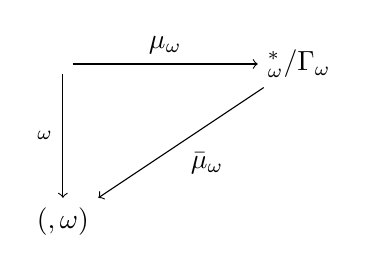
\begin{tikzpicture}[auto]
      \node (A)  at (0,0) {$\X$};
      \node (B)  at (3,0) {$\cG^*_\omega/\Gamma_\omega$};
      \node (C)  at (0,-2) {$\Chars(\X,\omega)$};
      \draw[->] (A) to node {$\mu_\omega$} (B);
      \draw[->] (A) to node [swap] {$\chars_\omega$} (C);
      \draw[->] (B) to node {$\bar\mu_\omega$} (C);
    \end{tikzpicture}
    \end{center}
    This construction is related to the
    well-known Marsden-Weinstein symplectic reduction \cite{MaWe74}, 
    when it is applied to some subspaces $\W \subset \X$ for the restriction 
    $\omega \restriction \W$. There is, however, a small difference:
    we reduce first by the characteristics of $\omega$ and then
    by the moment map, which can be interpreted as a {\em regularization} of
    the reduction by the characteristics\footnote{It is not impossible that
    in particular, for the two-bodies problem \cite{Sou83}, it be precisely 
    the universal moment map which regularizes the space of motions.}. 
  \end{article} %% The-characteristics-of-moment-maps
  

  %%%%%%%%%%%%%%%%%%%%%%%%%%%%%%%%%%%%%%%%%%%%%%%%%%%%%%%%%%

  \section*{The Homogeneous Case}
  \label{sec-The-homogeneous-case}
  
  \begin{sechead}
    Because of its simple character, the case of
    a homogeneous action of a diffeological group
    $\G$ on a space $\X$, preserving a closed $2$-form $\omega$,
    deserves a special attention. We shall see in
    \art{Symplectic-manifolds-are-coadjoint-orbits} how this
    applies to classical symplectic geometry.
  \end{sechead}
  
  \begin{article}\artlabel{The homogeneous case} 
    \addcontentsline{toc}{section}{\small\hspace{10pt} The homogeneous case} 
    \label{The-homogeneous-case} 
    Let $\X$ be a connected
    diffeological space equipped with a closed $2$-form
    $\omega$. Let $\rho$ be a smooth action of a
    diffeological group $\G$ on $\X$, preserving $\omega$.
    Let us assume that $\X$ is homogeneous for this action
    \art{Transitivity-and-homogeneity}. Let
    $\Gamma$ be the holonomy of the action $\rho$, let $\mu$
    be a moment map, and let $\theta$ be the cocycle associated
    to $\mu$. Let $x_0$ be any point of $\X$, and let $\mu_0
    = \mu(x_0)$. Let $\Stab_{\Ad_*^{\Gamma,\theta}}(\mu_0)$
    be the stabilizer of $\mu_0$ for the affine coadjoint
    action of $\G$ on $\cG^*\!/\Gamma$. Thanks to the
    equivariance of the moment map $\mu$, with respect to the
    $\theta$-affine coadjoint action of $\G$ on
    $\cG^*\!/\Gamma$, $\mu \circ \rho(g) =
    \Ad_*^{\Gamma,\theta}(g) \circ \mu$, the image $\cO =
    \mu(\X)$ is a $(\Gamma,\theta)$-orbit of $\G$, and
    $\Stab_\rho(x_0) \subset \Stab_{\Ad_*^{\Gamma,\theta}}(\mu_0)$. 
    Let us equip $\cO$ with the pushforward of the diffeology of $\G$ 
    by the orbit map $\hat\mu_0 : g \mapsto \Ad_*^{\Gamma,\theta}(g)(\mu_0)$. 
    Then, the orbit
    map $\hat x_0 : \G \to \X$ is a principal fibration with
    structure group $\Stab_\rho(x_0)$, the orbit map $\hat \mu_0 : \G \to \cO$ 
    is a principal fibration with
    structure group $\Stab_{\Ad_*^{\Gamma,\theta}}(\mu_0)$,
    and the moment map $\mu : \X \to \cO$ is a fibration, with fiber the
    homogeneous space
    $\Stab_{\Ad_*^{\Gamma,\theta}}(\mu_0)/\Stab_\rho(x_0)$.

    \Note{1} The moment maps $\mu$ are defined up to a
    constant. But the characteristics of $\mu$, that is,
    the connected components of the subspaces defined by
    $\mu(x) = \const$, are  not 
    \art{The-characteristics-of-moment-maps}.
    
    \Note{2} Let us consider the simple case $d\alpha$, where $\alpha \in \cG^*$.
    Its moment map $\mu : \G \to \cG^*$ is the coadjoint orbit map 
    $\mu : g \mapsto  \Ad_*(g)(\alpha)$.
    A natural question is then: is there a closed $2$-form
    $\omega$, defined on the coadjoint orbit $\cO_\alpha = \mu(\G)$, 
    such that $\mu^*(\omega) = d\alpha$\,?
    I have not a definitive answer yet to this question, the best I can say 
    is contained in the following proposition. Let us consider $\cO_\alpha$, equipped
    with the quotient diffeology of $\G$.
    
    \Proposition~There exists a closed $2$-form $\omega$ on $\cO_\alpha$ 
    such that $\mu^*(\omega) = d\alpha$, 
    if and only if $\alpha \restriction \Stab_{\Ad_*}(\alpha)$ is closed.

    \alinea{}There are particular cases, or special group diffeologies, 
    for which the restriction of $\alpha$ on its stabilizer
    $\Stab_{\Ad_*}(\alpha)$ is closed. For example, if $\G$ is a Lie group, 
    then we can use the Cartan formula to check it. But even simpler, if the stabilizer
    $\Stab_{\Ad_*}(\alpha)$ is discrete or $1$-dimensional, then every $1$-form is closed. 
    Paul Donato has given in \cite{Don94} an interesting example of discrete stabilizer. 
    Let us give here the diffeological version of his construction. 
    We consider $\G = \Diff(\S^1)$ and its universal covering $\tilde\G$ described in 
    \exref{Subduction-onto-diffeomorphisms} as the 
    subgroup of diffeomorphisms $\varphi$ of $\RR$ such that 
    $\varphi(x + 2\pi) = \varphi(x) + 2\pi$. The kernel of the projection $\pi : \tilde \G \to \G$
    is the subgroup $2\pi \ZZ$ of the translations $\T_{2\pi k} : x \mapsto x + 2\pi k$, 
    commuting with all $\varphi \in \tilde\G$. 
    Let $\P : \U \to \tilde\G$ be an $n$-plot, 
    let $r \in \U$, $\delta r \in \RR^n$, and $\alpha$ defined by
    $$
    \alpha(\P)_r(\delta r) = \sum_{n=0}^\infty {1 \over 2^n} 
    {\partial \over \partial s}\bigg\{\P(r)^{-1} \circ \P(s)(n)\bigg\}_{s=r} (\delta r).
    $$
    One can check that $\alpha$ is a left invariant $1$-form, and
    by the way an element of $\cG^*$. The moment map $\mu$ is then given by
    $$
    \mu(\varphi)(\P)_r(\delta r) = \sum_{n=0}^\infty {1 \over 2^n} 
    {\partial \over \partial s}\bigg\{\varphi^{-1} \circ \P(r)^{-1} 
    \circ \P(s) \circ \varphi (n)\bigg\}_{s=r} (\delta r).
    $$
    Because a momentum is characterized by its values on arcs centered at the identity, 
    and because every arc $\gamma$ centered at the identity in $\tilde \G$ is tangential
    to some ray $h \in \DHom(\RR,\tilde\G)$, the computation of the stabilizer of 
    $\alpha$, for the coadjoint action, is 
    reduced to Donato's computation in his paper, 
    and it coincides with the orbits of $2\pi\ZZ$.  
    Thus, $d\alpha$ passes to the coadjoint orbit $\cO_\alpha$, 
    which is actually diffeomorphic to $\Diff(\S^1)$ itself, 
    and symplectic according to the meaning we define below 
    \art{Symplectic-homogeneous-diffeological-spaces}.
  \end{article} %% The-homogeneous-case  
  
  \begin{proof}
    The triple fibration is an application of
    \art{Fibrations-of-groups-by-subgroups}. 
    \begin{center}
    \begin{tikzpicture}[auto]
      \node (A)  at (0,0) {$\G$};
      \node (B)  at (-2.5,-2.5) {$\X$};
      \node (C)  at (2.5,-2.5) {$\cO$};
      \draw[->] (A) to node [swap] {$\hat x_0$} (B);
      \draw[->] (A) to node {$\hat \mu_0$} (C);
      \draw[->] (B) to node [swap] {$\mu$} (C);
      \node (D)  at (6,0) {$\G$};
      \node (E)  at (3.5,-2.5) {$\X$};
      \node (F)  at (8.5,-2.5) {$\cO$};
      \draw[->]  (D) to node [swap] {$\Stab_\rho(x_0)$} (E);
      \draw[->]  (D) to node {$\Stab_{\Ad_*^{\Gamma,\theta}}(\mu_0)$} (F);
      \draw[->]  (E) to node [swap] {$\Stab_{\Ad_*^{\Gamma,\theta}}(\mu_0)/\Stab_\rho(x_0)$} (F);
    \end{tikzpicture}
    \end{center}
    Let us focus on note 2.
    There exists a (closed) $2$-form $\omega$ on $\cO_\alpha$
    such that $\mu^*(\omega) = d\alpha$ if and only if, 
    for two plots $\P$ and $\P'$ of $\G$ such that $\mu \circ \P = \mu \circ \P'$,
    then $d\alpha(\P) = d\alpha(\P')$ \art{Pushing-forms-onto-quotients}. But 
    $\mu \circ \P = \mu \circ \P'$ means that there exists a plot $\kappa$ of 
    $\Stab_{\cG^*}(\alpha)$ such that $\P'(r) = \P(r) \cdot \kappa(r)$. 
    Then, thanks to \exref{Pullback-of-1-forms-by-multiplication}, 
    $\alpha[r \mapsto \P(r)\cdot \kappa(r)]_r =
    [\eL(\P(r))^*(\alpha)](\kappa)_r + [\eR(\kappa(r))^*(\alpha)](\P)_r =
    \alpha(\kappa)_r + [\Ad_*(\kappa(r))(\alpha)](\P)_r$, but since $\kappa$ 
    is a plot of the stabilizer of $\alpha$ for the coadjoint action, 
    $\Ad_*(\kappa(r))(\alpha) = \alpha$ and $\alpha(\P') = \alpha(\P) + \alpha(\kappa)$.
    Thus, $d\alpha$ passes to the quotient $\cO_\alpha \simeq \G/\Stab_{\cG^*}(\alpha)$
    if and only if $d\alpha(\kappa) = 0$ for all plots $\kappa$ of $\Stab_{\cG^*}(\alpha)$,
    \ie, if and only if $d[\alpha \restriction \Stab_{\cG^*}(\alpha)] = 0$. 
  \end{proof}
  
  \begin{article}\artlabel{Symplectic homogeneous diffeological spaces}
    \addcontentsline{toc}{section}{\small\hspace{10pt} Symplectic homogeneous diffeological spaces} 
    \label{Symplectic-homogeneous-diffeological-spaces}
    Let $\X$ be a connected diffeological space and $\omega$
    be a closed $2$-form defined on $\X$.  
    
    \Definition~We say that $(\X,\omega)$ is a
    {\em homogeneous symplectic space} if it is homogeneous
    under the action of $\Diff(\X,\omega)$ and if the
    characteristics of a universal moment map $\mu_\omega$
    are reduced to points \art{The-characteristics-of-moment-maps}.
    
    \alinea{}For example, the $2$-form $d\alpha$ on $\Diff(\S^1)$ described in 
    the previous article \art{The-homogeneous-case} is symplectic in this sense.
    Let us recall that being homogeneous under the action of $\Diff(\X,\omega)$ 
    means that the orbit map $\orb{x} : \Diff(\X,\omega) \to \X$, defined by 
    $\orb{x}(\varphi) = \varphi(x)$, is a subduction, where $x \in \X$
    and  $\Diff(\X,\omega)$ is equipped with the functional diffeology 
    \art{Functional-diffeology-on-groups-of-diffeomorphisms}.
    
    \Note{1} The characteristics of a universal moment map
    $\mu_\omega$ are reduced to points if and only if it is a covering
    onto its image, equipped with the quotient diffeology. 
    If it is the case for one universal moment map, then
    is the case for everyone.
    
    \Note{2} The homogeneous situation where a
    moment map $\mu_\omega$ is not a covering onto its
    image can be regarded as the {\em presymplectic homogeneous case}, 
    as it is suggested by \art{Presymplectic-homogeneous-manifolds}.
    
    \Note{3}
    Let $\G$ be a diffeological
    group, and let $\rho$ be a smooth action of
    $\G$ on $\X$, preserving $\omega$. If the action
    $\rho$ of $\G$ on $\X$ is homogeneous, then $\X$ is a
    homogeneous space of $\Diff(\X,\omega)$. And, if a moment
    map $\mu : \X \to \cG^*\!/\Gamma$ is a covering onto its
    image, then any universal moment map $\mu_\omega : \X \to
    \cG^*_\omega/\Gamma_\omega$ is  a covering onto its
    image. Thus, to check that a homogeneous pair
    $(\X,\omega)$ is symplectic it is sufficient to find a
    homogeneous smooth action, of some
    diffeological group $\G$, for which a moment map
    is  a covering onto its image.
  \end{article} %% Symplectic-homogeneous-diffeological-spaces
  
  \begin{proof}
    The note 1 is obvious, by definition of the characteristics 
    \art{The-characteristics-of-moment-maps}
    and by homogeneity \art{The-homogeneous-case}. 
    Let us prove the note 3. To
    be homogeneous under the action of $\G$ means that, for
    some point (and thus for every point) $x \in \X$, the orbit
    map $\hat x : \G \to \X$, defined by $\hat x (g) =
    \rho(g)(x)$, is a subduction. So, $\hat x$ is surjective
    and, for any plot $\P : \U \to \X$, for any $r_0 \in \U$,
    there exist an open neighborhood $\V$ of $r_0$ and a plot $\Q : \V
    \to \G$ such that $\P \restriction \V = \hat x \circ \Q$,
    that is, $\P(r) = \rho(\Q(r))(x)$ for all $r \in \V$.
    Since $\rho$ is smooth, $\bar \Q = \rho \circ \Q$ is a
    plot of $\Diff(\X,\omega)$, and $\P \restriction \V =
    \hat x \circ \bar \Q$. Since, $\hat x : \Diff(\X,\omega)
    \to \X$ is surjective, it is a subduction and $\X$ is 
    a homogeneous space of $\Diff(\X,\omega)$. 
    %
    Now, let us remark that, since the moment maps differ only
    by a constant, if a moment map $\mu$ is a covering onto
    its image $\cO$ equipped with the quotient diffeology of
    $\G$, then every other moment map $\mu' = \mu + \const$
    is a covering onto its image $\cO' = \cO + \const$. Then,
    let $x_0$ be a point of $\X$, and let $\mu(x) =
    \psi(x_0,x)$, where $\psi$ is the $2$-points moment map.
    Let $\mu_\omega = \psi_\omega(x_0,x)$. According to
    \art{Universal-moment-maps}, 
    $\mu = \rho^*_{\Gamma_\omega} \circ \mu_\omega$. Let $\cO =
    \mu(\X) = \rho^*_{\Gamma_\omega} (\mu_\omega(\X)) = \rho^*_{\Gamma_\omega}(\cO_\omega)$,
    with $\cO_\omega = \mu_\omega(\X)$. 
    Let $m_\omega \in \cO_\omega$ and $m = \rho^*_{\Gamma_\omega}(m_\omega)$.
    If $\mu_\omega(x) = m_\omega$, then 
    $\rho^*_{\Gamma_\omega}(\mu_\omega(x)) = \rho^*_{\Gamma_\omega}(m_\omega)$,
    that is, $\mu(x) = m$. Thus, $\mu_\omega^{-1}(m_\omega) \subset \mu^{-1}(m)$.
    Therefore, if $\mu^{-1}(m)$ is discrete, then $\mu_\omega^{-1}(m_\omega)$ 
    is discrete, {\em a fortiori\/}, and if $\mu$ is injective, then $\mu_\omega$ is injective.
  \end{proof}
    
  %%%%%%%%%%%%%%%%%%%%%%%%%%%%%%%%%%%%%%%%%%%%%%%%%%%%%%%%%%
  %
  %   Exercises 
  %
  %%%%%%%%%%%%%%%%%%%%%%%%%%%%%%%%%%%%%%%%%%%%%%%%%%%%%%%%%%
  \Exercise
  
  \begin{exercise}[Compact supported real functions III]
    \label{Compact-supported-real-functions-III} Let us
    consider the space $(\X, \omega)$ as defined in
    \exref{Compact-supported-real-functions-I}. Show that
    $(\X,\omega)$ is a homogeneous symplectic space.
  \end{exercise} %% Compact-supported-real-functions-III
  
  \clearpage
  
  %%%%%%%%%%%%%%%%%%%%%%%%%%%%%%%%%%%%%%%%%%%%%%%%%%%%%%%%%%

  \section*{About Symplectic Manifolds}
  \label{About-Symplectic-Manifolds}
  
  \begin{sechead}
    The case of classical symplectic manifolds $(\M, \omega)$
    deserves a special care. We shall see in this section
    that, in this case, any universal moment map
    $\mu_\omega$ is injective and therefore identifies $\M$
    with a coadjoint orbit of
    $\Diff(\M,\omega)$, in the general meaning that we gave in
    \art{Affine-coadjoint-actions-and-orbits}.
  \end{sechead} 
  
  \begin{article}\artlabel{Value of the moment maps for manifolds} 
    \addcontentsline{toc}{section}{\small\hspace{10pt} Value of the moment maps for manifolds} 
    \label{Value-of-the-moment-maps-for-manifolds} 
    Let $\M$ be a connected manifold equipped with a closed
    $2$-form $\omega$. In this context, the paths moment map
    $\Psi_\omega$ takes a special expression. Let $p$ be a
    path in $\M$ and $\F : \U \to \Diff(\M,\omega)$ be 
    an $n$-plot, then
    \begin{equation}
      \renewcommand{\theequation}{$\diamondsuit$}
      \Psi_\omega(p)(\F)_r(\delta r) = \int_0^1
      \omega_{p(t)}(\dot p(t), \delta p(t)) \dt\,, 
    \end{equation}
    for all $r \in \U$ and $\delta r \in \RR^n$, where
    $\delta p$ is the lift in the tangent space $\T\M$ of
    the path $p$, defined by, 
    \begin{equation}\renewcommand{\theequation}{$\heartsuit$}
      \delta p(t) =
      [\D(\F(r))(p(t))]^{-1} {\partial \F(r)(p(t)) \over
      \partial r} (\delta r).
    \end{equation}
  \end{article} %% Value-of-the-moment-maps-for-manifolds
  
  \begin{proof}
    By definition, $\Psi(p)(\F) = \hat p^*(\CHK \omega)(\F) =
    \CHK \omega (\hat p \circ \F)$. The expression
    of the operator $\CHK$
    \art{The-Chain-Homotopy-operator-K}, applied to the plot
    $\hat p \circ \F : r \mapsto \F(r) \circ p$ of
    $\Paths(\X)$, gives
    $$
    (\CHK\omega)(\hat p \circ
    \F)_r(\delta r) = \int_0^1 \omega \left[ \vect{s \\ u} \mapsto (\hat p \circ \F)(u)(s + t) \right]_{s=0
    \choose u=r} \vect{1 \\ 0} \vect{0 \\ \delta r} \dt.
    $$
    But $(\hat p \circ \F)(u)(s + t)
    = \F(u)(p(s+t))$, let us denote temporarily by $\Phi_t$
    the plot $(s,u) \mapsto \F(u)(p(s+t))$, so $\F(u)(p(s+t))$
    writes $\Phi_t(s,u)$. Now, let us denote by $\cI$ the
    integrand  of the
    right term of this expression. We have,
    \begin{eqnarray*}
      \cI & = & \omega \left[ \vect{s \\ u} \mapsto \Phi_t(s,u) \right]_{s=0 \choose u=r} \vect{1 \\ 0} \vect{0 \\ \delta r} \\
      & = & \Phi_t^*(\omega)_{0 \choose r} \vect{1 \\ 0} \vect{0 \\ \delta r} \\ 
      & = & \omega_{\Phi_t{0 \choose r}} \left(\D(\Phi_t)_{0 \choose r} \vect{1 \\ 0},\D(\Phi_t)_{0 \choose r} \vect{0 \\ \delta v}\right) \\
      & =& \omega_{\F(r)(p(t))} \left({\partial \over \partial s} \bigg\{ \F(r)(p(s+t))\bigg\}_{s=0},{\partial  \over \partial r} \bigg\{\F(r)(p(t)) \bigg\} (\delta r)\right).
    \end{eqnarray*}
    But, 
    \begin{eqnarray*}
    {\partial \over \partial s} \bigg\{ \F(r)(p(s+t))\bigg\}_{s=0} & = &\D(\F(r))(p(t))\bigg({\partial p(s+t) \over \partial s}\bigg|_{s=0}\bigg) \\
    & =& \D(\F(r))(p(t))(\dot p(t)).
    \end{eqnarray*}
    Then, using this last expression and the fact that $\F$ is
    a plot of $\Diff(\M,\omega)$, that is, for all $r$ in $\U$,
    $\F(r)^*\omega = \omega$, we have
    \begin{eqnarray*}
      %\omega \left[\vect{s \\ u} \mapsto \Phi_t(s,u)\right]_{s=0 \choose u=r} 
      \cI & = & \omega_{\F(r)(p(t))}
      \bigg(\D(\F(r))(p(t))(\dot p(t)) , {\partial \F(r)(p(t))
      \over \partial r} (\delta r)\bigg) \\
      &=& \omega_{p(t)}
      \bigg(\dot p(t) , [\D(\F(r))(p(t))]^{-1}{\partial
      \F(r)(p(t)) \over \partial r} (\delta r)\bigg) \\
      &=& \omega_{p(t)}
      (\dot p(t) , \delta p(t)).
    \end{eqnarray*}
    Therefore, $\Psi_\omega(p)(\F)_r(\delta
    r) = \CHK \omega (\hat p \circ \F)_r(\delta r) =
    \displaystyle{\int_0^1} \omega_{p(t)}(\dot p(t), \delta
    p(t)) \dt$. \end{proof}
  
  \begin{article}\artlabel{The paths moment map for symplectic manifolds} 
    \addcontentsline{toc}{section}{\small\hspace{10pt} The paths moment map for symplectic manifolds} 
    \label{The-paths-moment-map-for-symplectic-manifolds} 
    Let $\M$ be a Hausdorff manifold and $\omega$ be a 
    nondegenerate closed $2$-form defined on $\M$. Let $m_0$ and
    $m_1$ be two points of $\M$ connected by a path $p$. Let
    $f \in \Cinfty(\M,\RR)$ with compact support. Let $\F$ be
    the exponential of the symplectic gradient\footnote{Let us recall that the symplectic gradient is defined by
    $\omega(\grad_\omega(f),\cdot) = -df$.}
    $\grad_\omega(f)$, $\F$ is a 1-plot of
    $\Diff(\M,\omega)$, and precisely a $1$-parameter
    homomorphism. Then, the universal paths moment map
    $\Psi_\omega$, computed at the path $p$, evaluated on the
    1-plot $\F$, is the constant $1$-form of $\RR$
    $$
    \Psi_\omega(p)(\F) = [f(m_1) -f(m_0)] \times dt
    \qmbox{with} \F :t \mapsto e^{t \grad_\omega(f)},
    $$
    where $dt$ is the standard $1$-form of $\RR$. Note that we are
    in the special case where $\F$ is actually a
    $1$-parameter homomorphism of
    $\Ham(\M,\omega) \subset \Diff(\M,\omega)$, and the
    function $f$ is one {\em Hamiltonian} of $\F$.
  \end{article} %% The-paths-moment-map-for-symplectic-manifolds
  
  \begin{proof}
    Let us remark that, in our case, the lift
    $\delta p$ defined by 
    \xart{Value-of-the-moment-maps-for-manifolds}{$(\heartsuit)$} writes
    simply 
    $$
    \delta p(t) = [\D(e^{r \xi})(p(t))]^{-1}
    {\partial e^{r \xi}(p(t)) \over \partial r} (\delta r) =
    \xi(p(t)) \times \delta r,
    $$
    with  $\xi = \grad_\omega(f)$, and where $r$ and $\delta r$ are real numbers. 
    Thus, the expression
    \xart{Value-of-the-moment-maps-for-manifolds}{$(\diamondsuit)$} becomes
    
    \begin{eqnarray*}
      \Psi_\omega(p)(\F)_r(\delta r) & = & \int_0^1
      \omega_{p(t)}(\dot p(t), \xi(p(t)) \dt \times \delta r \\
      & = & \int_0^1
      \omega_{p(t)}(\dot p(t), \grad_\omega(f)(p(t))
      \dt \times \delta r\\
      & = & \int_0^1 df\left({d p(t) \over dt} \right) \dt \times \delta r \\
      & = & [f(p(1)) - f(p(0))] \times \delta r,
    \end{eqnarray*}
    that is, $\Psi_\omega(p)(\F) = [f(m_1) - f(m_0)] \times dt$.
  \end{proof}
  
  \begin{article}\artlabel{Hamiltonian diffeomorphisms of symplectic manifolds} 
    \addcontentsline{toc}{section}{\small\hspace{10pt} Hamiltonian diffeomorphisms of symplectic manifolds} 
    \label{Hamiltonian-diffeomorphisms-on-symplectic-manifolds}
   Let $(\M,\omega)$ be a connected Hausdorff symplectic
    manifold. According to Banayaga \cite{Ban78}, a
    diffeomorphism $f$ is said to be {\em Hamiltonian\/} if
    it can be connected to the identity $\id_\M$ by a smooth
    path  $t \mapsto f_t$ in $\Diff(\M, \omega)$ such that
    $$
    \omega(\dot f_t, \cdot) = d\phi_t \qmbox{with} \dot
    f_t(x) = {d \over ds}\bigg\{f_s
    \circ f_t^{-1}(x)\bigg\}_{s=t},
    $$
    where $(t,x) \mapsto \phi_t(x)$ is a smooth real
    function. If $f$ is
    Hamiltonian according to this definition, then it belongs
    to $\Ham(\M, \omega)$, as defined in
    \art{The-group-of-Hamiltonian-diffeomorphisms}.
    Conversely, any element $f$ of $\Ham(\M, \omega)$
    satisfies the above Banyaga's condition. Thus, the
    definition of Hamiltonian diffeomorphisms given in
    \art{The-group-of-Hamiltonian-diffeomorphisms} is a
    faithful generalization of the usual definition for
    symplectic manifolds.
  \end{article} %% Hamiltonian-diffeomorphisms-on-symplectic-manifolds
  
  \begin{proof}
    This proposition is a direct consequence of the
    general statement given in
    \art{Time-dependent-Hamiltonian} and the
    following comparison between the above $1$-parameter family
    of vector fields $\dot f_t$ and the family
    $\F_t$ of the \art{Time-dependent-Hamiltonian}.
    %
    Since $f_{t'} \circ f_t^{-1} = f_t \circ (f_t^{-1}
    \circ f_{t'}) \circ f_t^{-1}$, the vector fields $\dot
    f_t$ and $\F_t$ are conjugated by $f_t$, precisely
    $$
    \dot f_t = (f_t)_*(\F_t) \qmbox{or} \dot f_t(x) =
    \D(f_t)(f_t^{-1}(x))(\F_t(f_t^{-1}(x))).
    $$
    This implies in particular that if the vector field
    $\dot f_t$ satisfies Banyaga's condition for the function
    $\phi_t$, then the vector field $\F_t$ satisfies Banyaga's
    condition for the function $\Phi_t = -\phi_t \circ
    f_t$, and conversely, that is,
    $$
    \omega(\dot f_t, \cdot) = d\phi_t \quad
    \Leftrightarrow \quad \omega(\F_t, \cdot) = - d\Phi_t
    \qmbox{with} \Phi_t = - \phi_t \circ f_t.
    $$
    Let us check it. Let $x \in \M$, $x' = f_t(x)$, $\delta x \in \T_x
    \M$, and $\delta x' = \D(f_t)(x)(\delta x)$, then
    \begin{eqnarray*}
      \omega_{x'} (\dot f_t(x'), \delta x') & =&
      [d\phi_t]_{x'}(\delta x') \\
      \omega_{f_t(x)}(\dot f_t (f_t(x)), \D(f_t)(x)(\delta x)) 
      & =& [d\phi_t]_{f_t(x)}(\D(f_t)(x)(\delta x))  \\
      \omega_{f_t(x)}(\D(f_t)(x)(\F_t(x)), \D(f_t)(x)(\delta
      x))  & =&  [f_t^*(d\phi_t)]_x(\delta x) \\
      {[f_t^*(\omega)]}_x(\F_t(x), \delta x) &=&
      d[f_t^*(\phi_t)]_x(\delta x) \\
      \omega_x(\F_t(x),\delta x) &
      = & d[\phi_t \circ f_t]_x(\delta x).
    \end{eqnarray*}
    Thus, $\Phi_t = - \phi_t \circ f_t$. 
  \end{proof}
  
  \begin{article}\artlabel{Symplectic manifolds are coadjoint orbits} 
    \addcontentsline{toc}{section}{\small\hspace{10pt} Symplectic manifolds are coadjoint orbits} 
    \label{Symplectic-manifolds-are-coadjoint-orbits} 
    Let $\M$ be a manifold and $\omega$ be a closed $2$-form defined on $\M$.
    We assume $\M$ connected and Hausdorff. Then, the form
    $\omega$ is nondegenerate, thus symplectic, if and
    only if  the two following conditions are fulfilled.
    
    \begin{itemize} 
      \item[A.] The manifold $\M$ is a homogeneous space of 
      $\Diff(\M,\omega)$.\vspace{3pt}
      
      \item[B.] The universal moment map 
      $\mu_\omega : \M \to \cG^*_\omega/\Gamma_\omega$ is
      injective. 
      
    \end{itemize}
    In that case, the image 
    $\cO_\omega = \mu_\omega(\M) \in \cG^*_\omega/\Gamma_\omega$
    of the universal moment map\footnote{The universal
    moment maps are defined up to a constant, but if one is injective, 
    then they are all injectives.} \art{Universal-moment-maps}
    is a $(\Gamma_\omega,\theta_\omega)$-coadjoint orbit of
    $\Diff(\M,\omega)$ \art{Affine-coadjoint-actions-and-orbits}, 
    and $\mu_\omega$ identifies $\M$ with
    $\cO_\omega$, where $\cO_\omega$ is equipped with the
    quotient diffeology of $\Diff(\M,\omega)$. In other
    words, {\em every symplectic manifold is a coadjoint orbit}. 
    
    \Note{1} Let $\Ham(\M,\omega)$ be the group of
    Hamiltonian diffeomorphisms, and $\cH^*_\omega$
    be the space of its momenta. Let 
    $\mu_\omega^\star : \M \to \cH^*_\omega$ 
    be a moment map associated with the
    action of $\Ham(\M,\omega)$, and
    $\theta_\omega^\star$ be the associated Souriau cocycle.
    Then, $\mu_\omega^\star$ is also injective, and identifies
    $\M$ to a $\theta_\omega^\star$-coadjoint orbit
    $\cO^\star_\omega \subset \cH_\omega^*$ of
    $\Ham(\M,\omega)$.
    
    \Note{2} Let us consider the example $\M = \RR^2$
    and $\omega = (x^2 + y^2)\ dx \wedge dy$. Since $\RR^2$ is
    contractible, the holonomy $\Gamma_\omega$ is trivial
    \art{The-holonomy-group}. Next, $\omega$ is
    nondegenerate on $\RR^2 - \{0\}$,
    but degenerates  at the point $(0,0)$. Thus, $(0,0)$ is an
    orbit of the group $\Diff(\RR^2,\omega)$, and actually
    $\RR^2 -\{0\}$ is the other orbit. Hence, the
    universal moment map $\mu_\omega$ such that
    $\mu_\omega(0,0) = 0_{\cG_\omega^*}$ is equivariant
    \xart{The-Souriau-cocycle}{note 2}. Moreover, $\mu_\omega$ is
    injective. The closed $2$-form $\omega$ not being symplectic, with an injective
    universal moment map, shows that the
    hypothesis of transitivity of $\Diff(\M,\omega)$ on $\M$
    is not superfluous is this proposition.
  \end{article} %% Symplectic-manifolds-are-coadjoint-orbits
  
  \begin{proof}
    Let us assume first that $\omega$ is nondegenerate, that is, symplectic. 
    Then, the group $\Diff(\M,\omega)$ is
    transitive on $\M$ \cite{Boo69}. Moreover, for every $m
    \in \M$, the orbit map $\hat m : \varphi \mapsto
    \varphi(m)$ is a subduction \cite{Don84}. Thus, the image of the moment
    moment map $\mu_\omega$ is one orbit $\cO_\omega$ of the
    affine coadjoint action of $\G_\omega$ on
    $\cG^*_\omega/\Gamma_\omega$, associated with the cocycle
    $\theta_\omega$. Hence, the
    orbit $\cO_\omega$ being equipped with the quotient diffeology
    of $\G_\omega$, the moment map $\mu_\omega$ is a
    subduction.
    
    Now, let $m_0$ and $m_1$ be two points of $\M$ such
    that 
    $\mu_\omega(m_0) = \mu_\omega(m_1)$, that is,
    $\psi_\omega(m_0,m_1) = \mu_\omega(m_1) -
    \mu_\omega(m_0)   = 0$. Let $p \in
    \Paths(\M)$ such that $p(0)= m_0$ and $p(1) = m_1$. Thus,
    $\psi_\omega(m_0,m_1) = 0$ is equivalent to
    $\Psi_\omega(p) = \Psi_\omega(\ell)$, where $\ell$ is
    some loop in $\M$, we can choose $\ell(0)=\ell(1)=m_0$.
    Now, let us assume that $m_0 \neq m_1$. Since $\M$ is
    Hausdorff there exists a smooth real
    function $f \in \Cinfty(\M, \RR)$, with compact support,
    such that $f(m_0) = 0$ and $f(m_1) = 1$. Let us denote by
    $\xi$ the symplectic gradient field associated with $f$ and
    by $\F$ the exponential of $\xi$. Thanks to
    \art{The-paths-moment-map-for-symplectic-manifolds}, on
    the one hand we have $\Psi(p)(\F) = [f(m_1) - f(m_0)] \dt
    = \dt$, and on the other hand $\Psi_\omega(\ell)(\F) =
    [f(m_0) - f(m_0)] \dt = 0$. But $dt \neq 0$, thus
    $\psi_\omega(m_0,m_1) \neq 0$, and the moment map
    $\mu_\omega$ is injective. Therefore, $\mu_\omega$ is an
    injective subduction on $\cO_\omega$, that is, a
    diffeomorphism.
    
    Conversely, let us assume that $\M$ is 
    a homogeneous space of $\Diff(\M,\omega)$ and that
    $\mu_\omega$ is injective. Let us notice first that since
    $\Diff(\M,\omega)$ is transitive, the rank of $\omega$ is
    constant. In other words, $\dim (\ker(\omega)) = \const$.
    Now, let us assume $\omega$ degenerate, that is,
    $\dim(\ker( \omega)) \geq 1$. Since $m \mapsto
    \ker(\omega_m)$ is a smooth foliation, for every point $m$
    of $\M$ there exists a smooth path $p$ in $\M$ such that
    $p(0) = m$ and for $t$ belonging to a small interval
    around $0 \in \RR$, $\dot p (t) \neq 0$ and $\dot p(t)
    \in \ker(\omega_{p(t)})$ for all $t$ in this interval. Then,
    we can re-parametrize the path $p$ and assume now that
    $p$ is defined on the whole $\RR$ and satisfies  $p(0) =
    m$, $p(1) = m'$ with $m \neq m'$, and $\dot p(t) \in
    \ker(\omega_{p(t)})$ for all $t$. Next,  since $\dot p(t)
    \in \ker(\omega_{p(t)})$ for all $t$, using the
    expression
    \xart{Value-of-the-moment-maps-for-manifolds}{$(\diamondsuit)$}, we get
    $\Psi_\omega(p) = 0_{\cG^*_\omega}$, that is,
    $\mu_\omega(m) = \mu_\omega(m')$. But $m \neq m'$ and we
    assumed $\mu_\omega$ injective, this is a contradiction. 
    Thus, the kernel of $\omega$ is reduced to $\{0\}$, $\omega$ is
    nondegenerate, that is, symplectic.
    
    Let us prove the note 1. According to a Boothby's
    theorem, the group $\Ham(\M,\omega)$ acts transitively
    on $\M$ \cite{Boo69}. With respect to this group, and by
    construction, the holonomy is trivial: the associated
    paths moment map $\Psi_\omega^\star$ and the moment maps
    $\mu_\omega^\star$ take their values in the space
    $\cH^*_\omega$. Let $j : \Ham(\M,\omega) \to
    \Diff(\M,\omega)$ be the inclusion, thus the universal 
    holonomy $\Gamma_\omega$ is in the kernel of $j^*$, and
    we get a natural mapping $j^*_{\Gamma_\omega} :
    \cG^*_\omega/\Gamma_\omega \to \cH^*_\omega$. Now, the
    paths moment maps satisfy $\Psi_\omega^\star =
    j^*_{\Gamma_\omega} \circ \Psi_\omega$, and
    $\mu_\omega^\star = j^*_{\Gamma_\omega} \circ \mu_\omega$
    \art{Universal-moment-maps}. Then, since 
    \art{The-paths-moment-map-for-symplectic-manifolds}
    involves only plots of $\Ham(\X,\omega)$, the proof above
    applies {\em mutatis mutandis} to the Hamiltonian case and we
    deduce that the moment maps $\mu_\omega^\star$ are
    injective. By transitivity, they identify $\M$ with a
    $\theta_\omega^\star$-coadjoint orbit of
    $\Ham(\M,\omega)$.
    
    Let us finish by proving the second
    note, that is, the universal moment map $\mu_\omega$ of
    $\omega = (x^2 + y^2)\ dx \wedge dy$ is injective. First
    of all $\mu_\omega(0,0) = 0_{\cG^*}$. Now, if $z=(x,y)$
    and $z' =(x',y')$ are two different points of $\RR^2$ and
    different from $(0,0)$, then there is a smooth function with
    compact support contained in a small ball, not containing
    $(0,0)$ nor $z$, such that $f(z')=1$. Then, the
    $1$-parameter group generated by $\grad_\omega(f)$ belongs
    to $\Diff(\RR^2,\omega)$, and a similar argument as
    the one of the proof above shows that $\mu_\omega(z) \neq
    \mu_\omega(z')$. We still need to prove that if $z \neq
    (0,0)$, then $\mu_\omega(z) \neq 0_{\cG^*}$. Let us consider
    $p(t) = tz$ and $\F(r)$ be the positive rotation of angle
    $2\pi r$, where $r \in \RR$. The application of
    \xart{Value-of-the-moment-maps-for-manifolds}{($\diamondsuit$)}, computed at
    the point $r=0$ and applied to the vector $\delta r =1$,
    gives $(2\pi/3) (x^2+y^2)^2$ which is not zero. Therefore, the
    moment map $\mu_\omega$ is injective.
  \end{proof}
  
  \begin{article}\artlabel{The classical homogeneous case} 
    \addcontentsline{toc}{section}{\small\hspace{10pt} The classical homogeneous case} 
    \label{The-classical-homogeneous-case} 
    Let $(\M,\omega)$ be a symplectic manifold. Let $\G$ be a
    Lie group together with a homogeneous Hamiltonian action
    on $(\M,\omega)$, that is, the holonomy
    $\Gamma$ of $\G$ is trivial. For the sake of
    simplicity we assume $\M$ connected and $\G$
    a Lie subgroup of $\Diff(\M,\omega)$. By functoriality
    of the moment maps
    \art{Images-of-the-moment-maps-by-morphisms}, we know
    that if a moment map $\mu$ of $\G$ is injective, then every
    universal moment map $\mu_\omega$ is injective
    \art{Symplectic-manifolds-are-coadjoint-orbits}. But we are
    now in the opposite case, since $\omega$ is symplectic
    every universal moment map $\mu_\omega$ is injective,
    but what about $\mu$ ? This is actually the original case
    treated by Souriau in \cite{Sou70}. He showed that the
    moment map $\mu$ is a covering onto its image, which is
    some coadjoint orbit $\cO \subset \cG^*$ (affine or not)
    of $\G$. We give here the proof of this theorem, according
    to the present framework. This case is illustrated by the
    \exref{The-cylinder-and-SL2R}.
  \end{article} %% The-classical-homogeneous-case
  
  \begin{proof}
    Let $p$ be a path in $\M$ such that $\mu \circ p =
    \const$, that is, $\Psi(p) = 0_{\cG^*}$, where $\Psi$ is
    the paths moment map of $\G$. Then, for any $1$-parameter
    subgroup $\F\in \DHom(\RR,\G)$, 
    $\Psi(p)(\F)_r(\delta r) = 0$, for all $r$ and all $\delta
    r$ belonging to $\RR$. Adapting to our case the expression
    of $\Psi$ given in
    \art{Value-of-the-moment-maps-for-manifolds} we get 
    $$
    \int_0^1
    \omega_{p(t)}(\dot p(t), \Z(p(t))) \dt = 0 \qmbox{where}
    \Z(m) = \left. {\partial \F(t)(m) \over \partial t} \right
    |_{t=0}.
    $$
    Now, considering the
    $1$-parameter family of paths $p_s : t \mapsto p(st)$, the
    derivative of the above expression gives
    $\omega_{p(0)}(\dot p(0), \Z(p(0))) = 0$. But since $\G$
    is transitive, by running over all the $1$-parameter
    subgroups $\F$ of $\G$ we describe the whole tangent space
    $\T_m \M$, where $m = p(0)$. And since $\omega$ is
    nondegenerate, $\dot p(0) = 0$. The path $p$ is
    thus constant, $p(t) = m$ for all $t$ in $\RR$. Therefore
    the preimages of the values of the moment map $\mu$ are
    discrete. But, $\mu$ is a fibration, see
    \art{The-homogeneous-case}, thus $\mu$ is a covering
    \art{Fundamental-group-acting-on-coverings} onto its image
    which is, by transitivity, a coadjoint orbit.  
  \end{proof}
  
  \begin{article}\artlabel{The Souriau-N\oe ther theorem} 
    \addcontentsline{toc}{section}{\small\hspace{10pt} The Souriau-N\oe ther theorem} 
    \label{The-Souriau-Noether-theorem} 
    Let $\M$ be a manifold and $\omega$ be a closed $2$-form on
    $\M$. We say that two points $m$ and $m'$ are on the same
    {\em characteristic}\footnote{This is the classical
    definition of the characteristics in the case of a closed
    $2$-form $\omega$ defined on a manifold $\M$. They are the
    integral submanifolds of the distribution $m \mapsto
    \ker(\omega_m)$.} of $\omega$ if there exists a path $p$
    connecting $m$ to $m'$ such that $\dot p(t) \in
    \ker(\omega_{p(t)})$ for all $t$. Then, the universal
    moment maps $\mu_\omega$ are constant on the
    characteristics of $\omega$. 
    
    \Note{1}~In particular, for any
    smooth action of a diffeological group $\G$, preserving
    $\omega$, the moment maps $\mu$ are constant on the
    characteristics of $\omega$.
    
    \Note{2}~This is an analogue to the first {N\oe ther} theorem, 
    relating symmetries to conserved quantities for Lagrangian systems. 
    For a comprehensive expos\'e on the subject see the book of 
    Y. Kosmann-Schwarzbach \cite{YKS10}.
  \end{article} %% The-Souriau-Noether-theorem
  
  \begin{proof}
    We have $\mu_\omega(m') - \mu_\omega(m) =
    \psi_\omega(m,m') = \class(\Psi_\omega(p)) \in
    \cG^*_\omega/\Gamma_\omega$, where $p$ is any (smooth)
    path connecting $m$ to $m'$. Then, thanks to the
    hypothesis, we can use a path $p$ contained in the
    characteristic of $\omega$ containing $m$ and $m'$, that is, 
    $\dot p(t) \in \ker(\omega_{p(t)})$ for all $t$. Now,
    thanks to the explicit formula of
    \art{Value-of-the-moment-maps-for-manifolds}, for every
    $n$-plot $\F$ of $\Diff(\M,\omega)$, $n \in \NN$, for
    every $r \in \Dom(\F)$, for every $\delta r \in \RR^n$,
    $$
    \Psi_\omega(p)(\F)_r(\delta r) = \int_0^1
    \omega_{p(t)}(\dot p(t),\delta p(t)) \dt = \int_0^1 0
    \times dt = 0.
    $$
    Thus, $\Psi_\omega(p) = 0$ and therefore
    $\mu_\omega(m') = \mu_\omega(m)$. 
    The note is a consequence of the functoriality of the moment map
    \art{Universal-moment-maps}. Indeed, let $\rho$ be the morphism
    from $\G$ to $\Diff(\M,\omega)$, then the paths moment map
    $\Psi$, relative to $\G$, satisfies $\Psi =
    \rho^* \circ \Psi_\omega$. Thus, $\Psi_\omega(p) =
    0$ implies $\Psi(p) = 0$ which implies $\mu(m) =
    \mu(m')$, for any moment map $\mu$ relative to $\G$.
  \end{proof}
  
  \begin{article}\artlabel{Presymplectic homogeneous manifolds} 
    \addcontentsline{toc}{section}{\small\hspace{10pt} Presymplectic homogeneous manifolds} 
    \label{Presymplectic-homogeneous-manifolds} 
    Let $\M$ be a connected Hausdorff manifold and $\omega$
    be a closed $2$-form on $\M$. Let $\G \subset
    \Diff(\M,\omega)$ be a connected subgroup. If $\M$ is 
    a homogeneous space of $\G$, then
    the characteristics of $\omega$ are the connected
    components of the preimages of the moment maps
    $\mu$. 
    
    \Note~In particular, if $\M$ is a homogeneous
    space of $\Diff(\M,\omega)$, and thus of its identity
    component \art{Connected-homogeneous-spaces}, then the
    characteristics of $\omega$ are the connected components
    of the preimages of the values of a universal moment
    map $\mu_\omega$.  This justifies {\em a posteriori} the
    definition of the characteristics of moment maps, for the
    general case of homogeneous diffeological spaces, in
    \art{The-characteristics-of-moment-maps}. 
  \end{article} %% Presymplectic-homogeneous-manifolds
  
  \begin{proof}
    The N\oe ther-Souriau theorem states that if $m$ and $m'$ are on the same characteristic, 
    then  $\mu(m) = \mu(m')$ \art{The-Souriau-Noether-theorem}. We shall prove the converse
    in a few steps.
    
    \alinea{a)}~Let us consider first the case when the holonomy of
    $\Gamma$ is trivial, $\Gamma = \{0\}$.  Let us assume 
    $m$ and $m'$ connected by a path $p$ such that
    $\mu(p(t)) = \mu(m)$ for all $t$. Then, let $s \mapsto p_s$ 
    be defined by $p_s(t) = p(st)$, for all $s$ and $t$.
    We have $\mu(p_s(1)) = \mu(p_s(0))$, that is,
    $\Psi(p_s) = 0_\cG^*$, for all $s$. Thus, for all
    $n$-plots $\F$ of $\G$, for all $r \in \Dom(\F)$ and all
    $\delta r \in \RR^n$, $\Psi(p_s)(\F)_r(\delta r) = 0$, and hence
    $$
    0 = {\partial \Psi(p_s)(\F)_r(\delta r)
    \over \partial s} = {\partial \over \partial
    s} \int_0^1
    \omega_{p_s(t)}(\dot p_s(t),\delta p_s(t)) \dt =
    \omega_{p(s)}(\dot p(s), \delta p(s)),
    $$
    where $\delta p(t)$ is given
    by \xart{Value-of-the-moment-maps-for-manifolds}{($\heartsuit$)}.
    Next, let $v \in \T_{p(t)}(\M)$, then there exists
    a path $c$ of $\M$ such that $c(0) = p(t)$ and
    $dc(s)/ds|_{s=0} = v$. Since $\M$ is assumed
    homogeneous under the action of $\G$, there exists a
    $1$-plot $s \mapsto \F(s)$ centered at the identity, that is, 
    $\F(0) = \id_\M$, such that $\F(s)(p(t)) = c(s)$.
    Then, for $s=0$ and $\delta s = 1$, we get from
    \xart{Value-of-the-moment-maps-for-manifolds}{($\heartsuit$)},
    $$
    \delta p(t) = \id_{\T_{p(t)}\M}\left.{d\F(s)(p(t)) \over
    ds}\right|_{s=0} = \left. {dc(s) \over ds} \right|_{s=0} =
    v.
    $$
    Hence, for every $v \in \T_{p(t)}\M$, $\omega(\dot p(t), v)
    = 0$, \ie\/, $\dot p(t) \in \ker(\omega_{p(t)})$ for all
    $t$. Therefore, the connected components of the preimages
    of the values of the moment map $\mu$ are the
    characteristics of $\omega$.
    
    \alinea{b)}~Let us consider the general case. Let $\widetilde \M$
    be the universal covering of $\M$, $\pi : \widetilde \M
    \to \M$ the projection, and let $\tilde \omega =
    \pi^*(\omega)$. Let $\widehat \G$ be the group defined by
    $$
    \widehat \G = \{ \hat g \in \Diff(\widetilde \M,\tilde
    \omega) \mid \exists g \in \G
    \mbox{ and } \pi \circ \hat g = g \circ \pi \}.
    $$
    Let $\rho : \widehat \G
    \to \G$ be the morphism $\hat g \mapsto g$. The group
    $\widehat \G$ is an extension of $\G$ by the homotopy
    group $\pi_1(\M)$
    $$
    \id \rfl{} \pi_1(\M) \rfl{} \widehat \G \rfl{\rho} \G
    \rfl{} \id.
    $$
    
    \alinea{1.} --- The morphism $\rho$ is
    surjective. Let $g \in \G$, let $t \mapsto g_t$ be a
    smooth path in $\G$ connecting $\id_\G$ to $g$. Let
    $\tilde m \in \widetilde \M$ and $m = \pi(\tilde m)$, 
    the path $t \mapsto g_t(m)$ has a unique lift 
    $t \mapsto \tilde m_t$ in $\widetilde \M$ starting at $\tilde m$
    \art{Monodromy-theorem}. We can check that, 
    $\tilde g : \tilde m \mapsto \tilde m_1$ is a
    diffeomorphism of $\widetilde \M$, satisfying by
    construction $\pi \circ \tilde g = g \circ \pi$. Next,
    $\tilde g^*(\tilde \omega) = \tilde g^*(\pi^*(\omega)) =
    \tilde g^* \circ \pi^* (\omega) = (\pi \circ \tilde
    g)^*(\omega) = (g \circ \pi)^*(\omega) =
    \pi^*(g^*(\omega)) = \pi^*(\omega) = \tilde \omega$. Thus,
    $\tilde g \in \widehat \G$.
    
    \alinea{2.} --- The group $\widehat \G$ is
    transitive on $\widetilde \M$. Let $\tilde m$ and $\tilde
    m'$ be two points of $\widetilde \M$, let $m =\pi(\tilde
    m)$ and $m' = \pi(\tilde m')$. Since $\G$ is transitive
    on $\M$ there exists $g \in \G$ such that $g(m) = m'$.
    The lift $\tilde g$ defined in the part 1 maps $\tilde
    m$ to $\tilde m_1$ and we have $\pi(\tilde m_1) =
    \pi(\tilde m') = m'$. So there exists an element $k \in
    \pi_1(\M)$ such that $k_{\tilde \M}(\tilde m_1) = \tilde m'$
    \art{The-universal-covering}. 
    Let $\hat g = k_{\tilde \M} \circ \tilde g$, since
    $\pi \circ \hat g = g \circ \pi$ and 
    $\hat g^*(\tilde \omega) = (k_{\tilde \M} \circ 
    \tilde g)^*(\tilde \omega) =  \tilde g^*(k_{\tilde \M}^*(\tilde \omega)) =
    \tilde g^*(\tilde \omega) = \tilde \omega$, 
    $\hat g$ belongs to $\widehat \G$,
    and maps $\tilde m$ to $\tilde m'$.
    
    \alinea{3.} --- The kernel of $\rho$ is reduced to
    $\pi_1(\M)$. Let $\tilde g \in \widehat \G$ such that
    $\rho(\tilde g) = \id_\M$, that is, $\pi \circ \tilde g =
    \pi$. Thus, for every $\tilde m \in \M$ there exists
    $\kappa(\tilde m) \in \pi_1(\M)$ such that $\tilde
    g(\tilde m) = \kappa(\tilde m)_\M(\tilde m)$. But the
    map $\kappa : \widetilde \M \to \pi_1(\M)$ is smooth, and
    $\pi_1(\M)$ discrete, so $\kappa$ is constant. Therefore,
    there exists $k \in \pi_1(\M)$ such that $\tilde g(\tilde
    m) = k_\M(\tilde m)$, for all $\tilde m \in \widetilde
    \M$. 
    
    \alinea{4.} --- Since $\widetilde \M$ is simply connected, 
    $\widehat \G$ has no holonomy. Let $\hat \mu$ be a
    moment map of the action of $\widehat \G$ on $\widetilde
    \M$. Since $\widehat \G$ is a discrete extension of $\G$,
    their space of momenta coincide
    \art{Momenta-and-connectedness}, thus $\hat \mu$ takes its
    values in $\cG^*$, and since the action of $\G$ on $\M$
    is the image by the morphism $\rho$ of the action of
    $\widehat \G$ on $\widetilde \M$, for every
    $\tilde m \in \widetilde \M$, $\mu(\pi(\tilde m)) =
    \class(\hat \mu(\tilde m)) \in \cG^*/\Gamma$
    \art{Pushing-forward-moment-maps}. Next, let $c = \mu(m) =
    \class(\hat \mu(\tilde m)) \in \cG^*/\Gamma$, $m =
    \pi(\tilde m)$, and $\C = \mu^{-1}(c)$. The preimage
    $\pi^{-1}(\C) = \pi^{-1}(\mu^{-1}(c))$ is equal to $(\mu
    \circ \pi)^{-1}(c) = (\class \circ \hat \mu)^{-1}(c) = 
    \hat \mu^{-1}(\class^{-1}(c)) = \hat \mu^{-1}(\hat
    \mu(\tilde m) + \Gamma)$. Thus,
    $$
    \mu^{-1}(c) = \pi\bigg(\bigcup_{\gamma \in \Gamma} \hat
    \mu^{-1}(\alpha + \gamma) \bigg) \qmbox{with}
    \alpha = \hat \mu(\tilde m) \qmbox{and} c =
    \class(\alpha).
    $$
    Since $\widehat \G$ is transitive on $\widetilde \M$
    and since there is no holonomy , we
    can apply the result of the part A: for every $\gamma \in
    \Gamma$, $\hat \mu^{-1}(\alpha + \gamma)$ is a union of
    characteristics of $\tilde \omega$. Thus, the union over
    all the $\gamma \in \Gamma$ is still a union of
    characteristics of $\omega$. Hence, $\mu^{-1}(c)$ is the
    $\pi$-projection of a union of characteristics
    of $\tilde \omega$. But, since $\pi : \widetilde \M \to
    \M$ is a covering and since $\tilde \omega =
    \pi^*(\omega)$, the $\pi$-projection of a
    characteristic of $\tilde \omega$ is a characteristic of
    $\omega$. Thus $\mu^{-1}(c)$ is a union of
    characteristics of $\omega$, and the connected components
    of the preimages of the values of $\mu$ are the
    characteristics of $\omega$.
  \end{proof}
  
  %%%%%%%%%%%%%%%%%%%%%%%%%%%%%%%%%%%%%%%%%%%%%%%%%%%%%%%%%%
  %
  %   Exercises 
  %
  %%%%%%%%%%%%%%%%%%%%%%%%%%%%%%%%%%%%%%%%%%%%%%%%%%%%%%%%%%
  
  \Exercises
  
  \begin{exercise}[The classical moment map]
    \label{The-classical-moment-map}
    Let $\M$ be a connected Hausdorff manifold equipped
    with a closed $2$-form $\omega$. Let $\G$ be a Lie group
    (that is, a diffeological group which is a manifold). Let
    $\rho : g \mapsto g_\M$ be a Hamiltonian action of $\G$
    on $\M$. Let us recall that a $1$-parameter subgroup $\F
    \in \DHom(\RR, \G)$ is uniquely defined by 
    $$
    \Z = \left. {d\F(t) \over dt} \right|_{t=0} \qmbox{and}
    \Z \in \cG = \T_{\id_\G}(\G).
    $$
    We denote $\F(t)=  e^{t\Z}$. The {\em fundamental
    vector field} $\Z_\M$ is defined on $\M$ by
    $$
    \Z_\M(m) = \left. {\partial e^{t\Z}_\M(m) \over \partial
    t} \right|_{t=0} \in \T_m(\M).
    $$
    Let $\mu$ be a moment
    map of the action of $\G$ on $\M$, we shall denote
    $$
    \mu_\Z(m) = \mu(m)(t\mapsto e^{tZ})_0(1).
    $$
    
    \Question{1)}~Show that the moment map $\mu$ is defined, up to a
    constant, by the differential equation 
    $$
    i_{\Z_\M}(\omega) = - d\mu_\Z, \quad \mbox{that is,} \quad
    \omega_m(\Z_\M(m), \delta m) = - d[\mu_\Z]_m(\delta m),
    $$
    for all $m \in \M$ and all $\delta m \in \T_m(\M)$. 
    
    \Question{2.}~Show then, using a basis of $\cG$, that $\Z \mapsto \mu_\Z$ is linear.
  \end{exercise} %% The-classical-moment-map
  
  \begin{exercise}[The cylinder and $\SL(2,\R)$]
    \label{The-cylinder-and-SL2R}
    We consider the space $\RR^2$, equipped
    with the standard symplectic form $\omega = dx \wedge dy$,
    with $\X = (x,y) \in \RR^2$. Check that the special linear
    group $\SL(2,\RR)$ preserves $\omega$, and that
    its action on $\RR^2$ has two orbits, the
    origin $0 \in \RR^2$ and the \guillemots{cylinder} $\M = \RR^2 -
    \{0\}$.

      \Question{1)} Justify, without computation, that the action of $\SL(2,\RR)$ on
       $\RR^2$ is Hamiltonian and exact.
       
      \Question{2)} For every $\X \in \RR^2$, let 
      $\gamma_\X = [t \mapsto t\X] \in \Paths(\RR^2)$ connecting $0$ to $\X$. Use the
      general expression of the paths moment map given in
      \art{Value-of-the-moment-maps-for-manifolds},
      for $p = \gamma_\X$ and $\F_\sigma = [s \mapsto
      e^{s\sigma}]$, with $\sigma \in \frak{sl}(2,\RR)$ --- the
      Lie algebra of $\SL(2,\RR)$, that is, the space of $2
      \times 2$ traceless matrices  --- to show that
      $$
      \mu(\X)(\F_\sigma) = \undemi \omega(\X,\sigma \X) \times dt.
      $$
      \Question{3)}~Deduce that the moment map $\mu_\M =
      \mu \restriction \M$ of $\SL(2,\RR)$ on $\M$ is a non
      trivial double sheets covering onto its image.
  \end{exercise} %% The-cylinder-and-SL2R
    
  %%%%%%%%%%%%%%%%%%%%%%%%%%%%%%%%%%%%%%%%%%%%%%%%%%%%%%%%%%
  
  \section*{Examples of Moment Maps in Diffeology}
  \addcontentsline{toc}{section}{\small\hspace{10pt} Examples of moment maps in diffeology} 
  \label{Examples-of-moment-maps-in-diffeology}
  
  \begin{sechead}
    The few following examples want to illustrate how the
    theory of moment maps in diffeology can be
    applied to the field of infinite dimensional
    situations, but also to the less familiar case of
    singular spaces. It is, at the same time, the opportunity to familiarize
    ourselves with the computational techniques in diffeology.
  \end{sechead}
  
  \begin{article}\artlabel{On the intersection 2-form of a surface I}
    \label{On-the-intersection-form-of-a-surface-I}
    Let $\Sigma$ be a closed surface oriented by a  $2$-form
    $\Surf$, chosen once and for all.
    Let us consider  $\Omega^1(\Sigma)$, the infinite
    dimensional vector space  of $1$-forms of $\Sigma$,
    equipped with the functional diffeology. Let us consider
    the antisymmetric bilinear map defined on
    $\Omega^1(\Sigma)$ by
    $$
    (\alpha,\beta) \mapsto \int_\Sigma \alpha\wedge \beta,
    $$
    for all $\alpha$, $\beta$ in $\Omega^1(\Sigma)$. Since
    the wedge-product $\alpha \wedge\beta$ is a $2$-form of
    $\Sigma$, there exists a real smooth function $\varphi \in
    \Cinfty(\Sigma,\RR)$ such that $\alpha \wedge \beta =
    \varphi \times \Surf$. Thus, by definition, $\int_\Sigma
    \alpha \wedge \beta = \int_\Sigma \varphi \times \Surf$. 
    
    \alinea{1.}~With the above bilinear form is naturally
    associated a well defined differential $2$-form $\omega$ of
    $\Omega^1(\X)$.  For every $n$-plot $\P : \U \to \X$,
    for all  $r \in \U$, $\delta r$ and $\delta' r$ in
    $\RR^n$,
    $$
    \omega(\P)_r(\delta r,\delta' r) = \int_\Sigma
    {\partial \P(r) \over \partial r}(\delta r)\wedge
    {\partial \P(r) \over \partial r}(\delta' r).
    $$
    
    \alinea{2.}~ The $2$-form $\omega$ is the differential of the $1$-form 
    $\lambda$ defined on $\Omega^1(\Sigma)$ by
    $$
    \lambda(\P)_r(\delta r) = \undemi \int_\Sigma
    \P(r)\wedge {\partial \P(r) \over \partial r}(\delta
    r) \qmbox{and} \omega = d\lambda.
    $$
    
    \alinea{3.}~ Consider now the additive group $(\Cinfty(\Sigma,\RR),+)$ of smooth
    real functions on $\Sigma$, and let us define the
    following action of $\Cinfty(\Sigma,\RR)$ on
    $\Omega^1(\Sigma)$,
    $$
    \mbox{for all $f \in \Cinfty(\Sigma,\RR)$}, \quad f
    \mapsto \bar f = [\alpha \mapsto  \alpha + df].
    $$
    Then, the additive group $\Cinfty(\Sigma,\RR)$ acts by
    automorphisms on the pair $(\Omega^1(\Sigma),\omega)$,
    $$
    \mbox{for all $f$ in $\Cinfty(\Sigma,\RR)$},
    \quad f^*(\omega) = \omega.
    $$
    Note that the kernel of the action $f \mapsto \bar f$ is the
    subgroup of constant maps, and the image of
    $\Cinfty(\Sigma,\RR)$ is the group
    $\BDR^1(\Sigma)$ of exact $1$-forms of $\Sigma$.
    
    \alinea{4.}~Let $p \in \Paths(\Omega^1(\Sigma))$ be a path
    connecting $\alpha_0$ to $\alpha_1$. The paths moment map
    $\Psi(p)$ is then given by
    $$
    \Psi(p) = \bigg(\hat \alpha_1^*(\lambda)
    + d\bigg[f \mapsto \undemi \int_\Sigma f
    \times d\alpha_1\bigg]\bigg) - \bigg(\hat
    \alpha_0^*(\lambda) + d\bigg[f \mapsto
    \undemi \int_\Sigma
    f \times  d\alpha_0 \bigg] \bigg).
    $$
    On this expression, we get immediately the
    $2$-points moment map $\psi(\alpha_0,\alpha_1) = \Psi(p)$, 
    for any path $p$ connecting $\alpha_0$ to $\alpha_1$.  Note that,
    since $\Omega^1(\Sigma)$ is 
    contractible, the holonomy of the action of
    $\Cinfty(\Sigma,\RR)$ is trivial, $\Gamma = \{0\}$, 
    and the action of $\Cinfty(\Sigma,\RR)$ is Hamiltonian.
    
    \alinea{5.}~The moment maps of this action of $\Cinfty(\Sigma,\RR)$ on
    $\Omega^1(\Sigma)$ are, up to a constant, equal to 
    $$
    \mu : \alpha \mapsto d \bigg[ f \mapsto \int_\Sigma
    f \times d\alpha\bigg].
    $$
    Moreover, the moment map $\mu$ is equivariant, that is,
    invariant, since the group $\Cinfty(\Sigma,\RR)$ is
    Abelian,
    $$
    \mbox{for all $f \in \Cinfty(\Sigma,\RR)$}, \quad \mu
    \circ \bar f = \mu.
    $$
    In summary, the action of $\Cinfty(\Sigma,\RR)$ on
    $\Omega^1(\Sigma)$ is exact and Hamiltonian.
    
    \Note~The moment
    map $\mu(\alpha)$ is fully characterized by $d\alpha$.
    This is why we find in the mathematical
    literature on the subject that the moment map for this
    action is the exterior derivative (or curvature,
    depending on the authors) $\alpha \mapsto d\alpha$. But
    as we see again on this example, the diffeological framework gives to this
    assertion a precise meaning.
    Let us also remark that the moment map
    $\mu$ is linear, for all real numbers $t$ and $s$, and for all $\alpha$
    and $\beta$ in $\Omega^1(\Sigma)$,
    $\mu(t\,\alpha+s\,\beta) = 
    t\,\mu(\alpha)+s\,\mu(\beta)$. The kernel
    of $\mu$ is the subspace of closed $1$-forms,
    $$
    \ker(\mu) = \ZDR^1(\Sigma) = \left\{ \alpha \in
    \Omega^1(\Sigma) \ \vert \ d\alpha = 0 \right\}.
    $$ 
    The orbit of the zero form $0 \in
    \Omega^1(\Sigma)$ by $\Cinfty(\Sigma,\RR)$ is just
    the subspace $\BDR^1(\Sigma) \subset \ZDR^1(\Sigma)$,
    see 
    \xart{On-the-intersection-form-of-a-surface-III}{note 3} for a discussion 
    about that.
  \end{article} %% On-the-intersection-form-of-a-surface-I
  
  \begin{proof}
    1. Let us check that $\omega$ defines a differential
    $1$-form on $\Omega^1(\Sigma)$. Note
    that, for any $r \in \U = \Dom(\P)$, $\P(r)$ is a section
    of the ordinary cotangent bundle $\T^*\Sigma$, 
    $\P(r) = [x \mapsto \P(r)(x)] \in
    \Cinfty(\Sigma,\T^*\Sigma)$, where $\P(r)(x) \in
    \T_x^*(\Sigma)$. Thus,
    $$
    {\partial \P(r) \over \partial
    r}(\delta r) = [x \mapsto  {\partial \P(r)(x) \over
    \partial r}(\delta r)] \quad \mbox{and} \quad {\partial
    \P(r) (x) \over \partial r}(\delta r) \in
    {\T}^{*}_{x}(\Sigma),
    $$
    where $\partial \P(r)(x) / \partial r$ denotes the
    tangent linear map $\D(r \mapsto \P(r)(x))(r)$. 
    The formula giving $\omega$ is then well defined. Now,
    $\omega(\P)_r$ is clearly antisymmetric and depends
    smoothly on $r$. Hence, $\omega(\P)$ is a smooth $2$-form
    of $\U$. Let us check that $\P \mapsto \omega(\P)$
    defines a $2$-form on $\Omega^1(\Sigma)$, that is,
    satisfies the compatibility condition $\omega(\P \circ
    \F) = \F^*(\omega(\P))$, for all $\F \in \Cinfty(\V,
    \U)$, where $\V$ is a real domain. Let $s \in \V$,
    $\delta s$ and $\delta' s$ two tangent vectors to $\V$ at $s$,
    let $r = \F(s)$, and compute:
    \begin{eqnarray*} 
      \omega(\P \circ \F)_s(\delta s,\delta' s) & = & \int_\Sigma {\partial \P \circ \F(s) \over \partial s}(\delta s)\wedge {\partial \P \circ \F(s) \over \partial s}(\delta' s)  
%      & = & \int_\Sigma {\partial \P(r) \over \partial r}{\partial \F(s) \over \partial s}(\delta s)\wedge {\partial \P(r) \over \partial r}{\partial  \F(s) \over \partial s}(\delta' s) \\
%      & = & \omega(\P)_{\F(s)}(\D\F_s(\delta s),\D\F_s(\delta' s)) \\
%      & = & \F^*(\omega(\P))_s(\delta s,\delta' s).
    \end{eqnarray*}
    \begin{eqnarray*} 
     \phantom{\omega(\P \circ \F)_s(\delta s,\delta' s)} % & = & \int_\Sigma {\partial \P \circ \F(s) \over \partial s}(\delta s)\wedge {\partial \P \circ \F(s) \over \partial s}(\delta' s) \\ 
     & = & \int_\Sigma {\partial \P(r) \over \partial r}{\partial \F(s) \over \partial s}(\delta s)\wedge {\partial \P(r) \over \partial r}{\partial  \F(s) \over \partial s}(\delta' s) \\
     & = & \omega(\P)_{\F(s)}(\D\F_s(\delta s),\D\F_s(\delta' s)) \\
     & = & \F^*(\omega(\P))_s(\delta s,\delta' s).
    \end{eqnarray*}
    Thus, $\omega(\P \circ \F) =
    \F^*(\omega(\P))$, and $\omega$ is a well
    defined $2$-form on $\Omega^1(\Sigma)$. 
    
    \alinea{2.}~First of all, the proof that the map $\P \mapsto
    \lambda(\P)$ is a well defined differential $1$-form of
    $\Omega^1(\Sigma)$ is analogous to the proof of the
    first item. Now, let us recall that $\omega = d\lambda$ 
    means $d(\lambda(\P)) = \omega(\P)$, for all plots
    $\P$ of $\Omega^1(\Sigma)$. Let us apply the usual
    formula of differentiation of $1$-forms on real domains,
    $$
    d\epsilon_r(\delta r,\delta' r) =
    \delta(\epsilon_r(\delta' r)) - \delta'(\epsilon_r(\delta
    r)),$$ 
    where $\delta$ and $\delta'$ are two independent
    variations. For the sake of simplicity let us denote 
    $$
    \alpha = \P(r), \quad \delta\alpha = {\partial \P(r)
    \over \partial r}(\delta r), \quad \delta'\alpha =
    {\partial \P(r) \over \partial r}(\delta' r).
    $$
    Then, 
    \begin{eqnarray*}
      d(\lambda(\P))_r(\delta r,\delta' r) & = & \undemi \bigg[\delta \int_\Sigma \alpha \wedge \delta' \alpha - \delta' \int_\Sigma \alpha \wedge \delta \alpha \bigg] \\
      & = & \undemi \bigg[\int_\Sigma \delta \alpha \wedge \delta' \alpha + \alpha \wedge \delta \delta' \alpha - \int_\Sigma \delta' \alpha \wedge \delta \alpha + \alpha \wedge \delta' \delta \alpha \bigg],
    \end{eqnarray*} 
    but $\delta \delta' \alpha = \delta' \delta \alpha$, thus
    \begin{eqnarray*}
      d(\lambda(\P))_r(\delta r,\delta' r) & = & \undemi \bigg[\int_\Sigma \delta \alpha \wedge \delta' \alpha - \int_\Sigma \delta' \alpha \wedge \delta\alpha \bigg] \\
      & = & \undemi \bigg[\int_\Sigma \delta \alpha \wedge \delta' \alpha + \int_\Sigma \delta \alpha \wedge \delta' \alpha \bigg] \\
      & = & \int_\Sigma \delta \alpha \wedge \delta' \alpha \\
      & = & \omega_r(\delta r,\delta' r).
    \end{eqnarray*}
    
    \alinea{3.}~Let us compute the pullback of $\lambda$ by the
    action of $f \in \Cinfty(\Sigma,\RR)$. Let $\P : \U \to
    \Omega^1(\Sigma)$ be an $n$-plot, let $r \in \U$ and
    $\delta r \in \RR^n$\,:
    \begin{eqnarray*}
      \bar f^*(\lambda)(\P)_r(\delta r) & = & \lambda( \bar f
      \circ \P)_r(\delta r) \\
      & = & \lambda(r \mapsto \P(r) + df)_r (\delta r) \\
      & = & \undemi \int_\Sigma (\P(r) + df) \wedge {\partial
      \P(r) \over \partial r}(\delta r) \\
      & = & \undemi \int_\Sigma \P(r) \wedge {\partial
      \P(r)\over \partial r}(\delta r) + \undemi \int_\Sigma df
      \wedge {\partial \P(r) \over \partial r}(\delta r) \\
      & = & \lambda(\P)_r(\delta r) + {\partial \over \partial
      r} \bigg\{\undemi \int_\Sigma df \wedge
      \P(r)\bigg\}(\delta r) \\
      & = & \lambda(\P)_r(\delta r) - {\partial \over \partial
      r}\bigg\{ \undemi \int_\Sigma f
      \times d(\P(r))\bigg\}(\delta r). \\
    \end{eqnarray*}
    Next, we define, for every $f \in \Cinfty(\Sigma,\RR)$, 
    $\varphi(f) : \Omega^1(\Sigma) \to \RR$ by
    $$
    \varphi(f) : \alpha  \mapsto \undemi \int_\Sigma f \times
    d\alpha.
    $$
    Then, 
    $$
    d(\varphi(f))(\P)_r(\delta r) = {\partial \over \partial
    r} \bigg\{ \undemi \int_\Sigma f
    \times d(\P(r)) \bigg\}(\delta r).
    $$
    Thus,
    $$ 
    \bar f^*(\lambda)(\P)_r(\delta r) =
    \lambda(\P)_r(\delta r)  -
    (d\varphi(f))(\P)_r(\delta r),
    $$
    that is,
    $$
    \bar f^*(\lambda) = \lambda - d(\varphi(f)).
    $$
    Hence, $d[\bar f^*(\lambda)] = d\lambda$, and  $\omega = d\lambda$ is
    invariant by the action of $\Cinfty(\Sigma,\RR)$. 
    
    \alinea{4.}~Let $p$ be a path in $\Omega^1(\Sigma)$ connecting
    $\alpha_0$ to $\alpha_1$. By definition $\Psi(p) =
    \hat p^*(\CHK\omega)$.
    Applying the property of the Chain-Homotopy
    operator $d \circ \CHK + \CHK \circ d = \1^* -
    \0^*$ to $\omega = d\lambda$, we
    get
    \begin{eqnarray*}
      \Psi(p) & = & \hat
      p^*(\CHK d\lambda) \\
      & = & \hat p^*(\1^*(\lambda) -
      \0^*(\lambda) - d (\CHK \lambda)) \\
      & = & (\1 \circ
      \hat p)^*(\lambda) - (\0 \circ \hat
      p)^*(\lambda) - d [(\CHK \lambda) \circ \hat p] \\
      & = & \hat \alpha_1^*(\lambda) - \hat
      \alpha_0^*(\lambda) - d[f \mapsto \CHK\lambda(\hat p(f))].
    \end{eqnarray*}
    But $\CHK\lambda(\hat p(f)) = \CHK\lambda(\bar f \circ
    p) = \int_{\bar f \circ p} \lambda = \int_p \bar
    f^*(\lambda)$, and since $\bar f^*(\lambda) = \lambda -
    d(\varphi(f))$, $\CHK\lambda(\hat p(f)) = \int_p
    \lambda - \int_p d(\varphi(f)) = \int_p \lambda
    - \varphi(f)(\alpha_1) + \varphi(f)(\alpha_0)$. Therefore,
    \begin{eqnarray*}
      \Psi(p) & = & \hat \alpha_1^*(\lambda) -
      \hat \alpha_0^*(\lambda) - d[f \mapsto -
      \varphi(f)(\alpha_1) + \varphi(f)(\alpha_0)] \\
      & = & \hat \alpha_1^*(\lambda) - \hat
      \alpha_0^*(\lambda) + d\bigg[ f \mapsto \undemi
      \int_\Sigma f \times d\alpha_1 - \undemi \int_\Sigma f
      \times d \alpha_0 \bigg].
    \end{eqnarray*}
    We get then the paths moment map $\Psi$,
    $$
    \Psi(p) =
    \bigg(\hat \alpha_1^*(\lambda) + d \bigg[f \mapsto
    \undemi \int_\Sigma f \times  d\alpha_1 \bigg]\bigg) -
    \bigg(\hat \alpha_0^*(\lambda) + d \bigg[f  \mapsto
    \undemi \int_\Sigma f \times d \alpha_0 \bigg]\bigg).
    $$
    Concerning the $2$-points moment map $\psi$, we clearly have
    $\psi(\alpha_0,\alpha_1) = \Psi(p)$, for any path
    connecting $\alpha_0$ to $\alpha_1$.
    
    \alinea{5.}~The $1$-point moment maps are given by $\mu(\alpha) =
    \psi(\alpha_0,\alpha)$ for any origin $\alpha_0$. Let us
    choose $\alpha_0 = 0$. So,
    $$
    \mu(\alpha) = \hat \alpha^*(\lambda) +
    d \bigg[f \mapsto \undemi \int_\Sigma f \times d\alpha
    \bigg] - \0^*(\lambda).
    $$
    But $\0^*(\alpha)$ is not necessarily zero. Let us
    compute generally $\hat \alpha^*(\lambda)$. Let $\P : \U
    \to \Omega^1(\Sigma)$ be an $n$-plot,
    $\hat \alpha^*(\lambda)(\P) =
    \lambda(\hat \alpha \circ \P) =  \lambda(r \mapsto
    \hat \alpha(\P(r)) = \lambda(r \mapsto 
    \alpha + d(\P(r)))$, and
    \begin{eqnarray*}
      \lambda(r \mapsto \alpha + d(\P(r))) & = &
      \undemi \int_\Sigma (\alpha + \P(r)) \wedge {\partial
      \over \partial r}(\alpha + d(\P(r))) \\
      & = &  \undemi \int_\Sigma (\alpha + \P(r)) \wedge
      {\partial d(\P(r)) \over \partial r} \\
      & = & \undemi \int_\Sigma \alpha \wedge {\partial
      d(\P(r)) \over \partial r} + \undemi \int_\Sigma
      \P(r) \wedge {\partial d(\P(r)) \over \partial r}. 
    \end{eqnarray*}
    Then,
    $$
    (\hat \alpha^*(\lambda) - \0^*(\lambda))(\P) = 
    \undemi \int_\Sigma \alpha \wedge {\partial d(\P(r)) \over
    \partial r}.
    $$
    Therefore, 
    \begin{eqnarray*}
      \mu(\alpha)(\P)_r & = & (\hat \alpha^*(\lambda) -
      \0^*(\lambda))(\P)_r + d \bigg[f \mapsto \undemi
      \int_\Sigma f \times d\alpha\bigg](\P)_r \\
      & = & \undemi \int_\Sigma \alpha \wedge {\partial
      d(\P(r)) \over \partial r} + {\partial \over \partial
      r} \bigg\{ \undemi \int_\Sigma \P(r) \times
      d \alpha \bigg\} \\
      & = & \undemi {\partial \over
      \partial r} \bigg\{ \int_\Sigma \alpha \wedge d(\P(r)) +
      \P(r) \times d\alpha \bigg\} \\
      & = & {\partial \over
      \partial r} \bigg\{ \int_\Sigma \P(r) \times d\alpha
      \bigg\},
    \end{eqnarray*}
    which gives finally 
    $$
    \mu(\alpha) = d \bigg[ f \mapsto \int_\Sigma f \times
    d\alpha \bigg].
    $$
    Now, let us express the variance of $\mu$. Let $f \in
    \Cinfty(\Sigma,\RR)$ and $\F(\alpha)$ be the real
    function $\F(\alpha) : f \mapsto \int_\Sigma f \times
    d\alpha$, such that $\mu(\alpha) = d\F(\alpha)$. We
    have $\mu(\bar f(\alpha)) =  \mu (\alpha + df) =
    d\F(\alpha + df)$ but, for every $h \in
    \Cinfty(\Sigma,\RR)$, $\F(\alpha + df)(h) = \int_\Sigma h
    \times d(\alpha + df) = \int_\Sigma h \times d\alpha =
    \F(\alpha)(h)$. Then, for all $f \in
    \Cinfty(\Sigma,\RR)$, $\mu \circ \hat f = \mu$.
    The moment map $\mu$ is invariant by the group
    $\Cinfty(\Sigma,\RR)$. The Souriau class is zero,
    the action of $\Cinfty(\Sigma,\RR)$ is then exact and
    Hamiltonian.
    
    Let us end with the computation of the kernel of the moment map
    $\mu$. Clearly, $\mu(\alpha) = 0$ if and only if 
    $d\F(\alpha) = 0$. But since $\Cinfty(\Sigma,\RR)$
    is connected (actually contractible as a diffeological
    vector space), $d\F(\alpha) = 0$ if and only if
    $\F(\alpha) = \const = \F(\alpha)(0) = 0$. But
    $\F(\alpha) = 0$ if and only if, for all
    $f \in \Cinfty(\Sigma,\RR)$, $\int_\Sigma f
    \times d\alpha = 0$, that is, if and only if $d\alpha =
    0$.
  \end{proof}
  
  \begin{article}\artlabel{On the intersection 2-form of a surface II} 
  \label{On-the-intersection-form-of-a-surface-II}
    We continue with the example of  
    \art{On-the-intersection-form-of-a-surface-I}, using the
    same notations. Let us introduce the
    group $\G$ of positive diffeomorphisms of
    $(\Sigma,\Surf)$, that is,
    $$
    \G = \bigg\{ g \in \Diff(\Sigma) \ \bigg| \ {g^*(\Surf)
    \over \Surf} >0 \bigg\}.
    $$
    The group $\G$ acts by pushforward on
    $\Omega^1(\Sigma)$. For all $g \in \G$, for all $\alpha
    \in \Omega^1(\Sigma)$, $g_*(\alpha) \in \Omega^1(\Sigma)$,
    and for all pairs $g$, $g'$ of elements of $\G$, $(g \circ
    g')_* = g_* \circ g'_*$, and this action is smooth. 

      \alinea{1.}~The pushforward action of $\G$ on
      $\Omega^1(\Sigma)$ preserves the $1$-form $\lambda$, and
      thus the $2$-form $\omega$. For all $g \in \G$,
      $(g_*)^*(\lambda) = \lambda$, and $(g_*)^*(\omega) =
      \omega$. Thus, the action of $\G$ is exact, $\sigma = 0$,
      and Hamiltonian, $\Gamma = \{0\}$.
      
      \alinea{2.}~The moment maps are, up to a constant, equal to
      the moment $\mu$, 
      $$ 
      \mu(\alpha)(\P)_r(\delta r) = \undemi \int_\Sigma
      \alpha \wedge \P(r)^*\bigg({\partial \P(r)_*(\alpha) \over
      \partial r}(\delta r)\bigg),
      $$
      for all $\alpha \in \Omega^1(\Sigma)$, for all $n$-plots
      $\P$, where $r \in \Dom(\P)$ and $\delta r \in
      \RR^n$. In particular, applied to any 1-plot $\F$
      centered at the identity $\id_\G$, that is, $\F(0) =
      \id_\G$, we get the special expression
      $$
      \mu(\alpha)(\F)_0(1) = - \undemi \int_\Sigma
      \alpha \wedge \DLie_\F(\alpha) = - \int_\Sigma
      i_\F(\alpha) \times d\alpha,
      $$
      where $\DLie_\F(\alpha)$ and $i_\F(\alpha)$ are the Lie derivative
      and the contraction of $\alpha$ by $\F$. Note that
    it is not surprising that the Lie derivative of $\alpha$ is 
    closely associated with the moment map of the action of the group of 
    diffeomorphisms.  
  \end{article} %% On-the-intersection-form-of-a-surface-II
  
  \begin{proof}
    1.  Let us compute the pullback of $\lambda$ by the
    action of $g \in \G$, that is, $(g_*)^*(\lambda)$. Let $\P
    : \U \to \Omega^1(\Sigma)$ be an $n$-plot, let $r \in \U$,
    and $\delta r \in \RR^n$, then
    \begin{eqnarray*}  (g_*)^*(\lambda)(\P)_r(\delta r) & = &
      \lambda(g_* \circ \P)_r(\delta r) \\
      & = & \undemi \int_\Sigma g_*(\P(r)) \wedge {\partial
      g_*(\P(r)) \over \partial r}(\delta r)\\
      & = & \undemi \int_\Sigma g_*(\P(r)) \wedge
      g_*\bigg({\partial \P(r) \over \partial r}(\delta
      r)\bigg) \\
      & = & \undemi  \int_\Sigma g_*\bigg(\P(r)\wedge
      {\partial \P(r) \over \partial r}(\delta r)\bigg) \\
      & = & \undemi  \int_{g^*(\Sigma)} \P(r)\wedge {\partial
      \P(r) \over \partial r}(\delta r) \\
      & = & \undemi \int_\Sigma \P(r)\wedge {\partial \P(r)
      \over \partial r}(\delta r) \\
      & = & \lambda (\P)_r(\delta r).
    \end{eqnarray*}
    Thus, $\lambda$ is invariant by $\G$, and so is $\omega =
    d\lambda$.
    
    \alinea{2.}~Since the $1$-form $\lambda$ is invariant by the
    action of $\G$, we can use directly the
    results of the exact case detailed in
    \art{The-exact-case}. The moment maps are, up to a
    constant, equal to $\mu : \alpha \mapsto \hat
    \alpha^*(\lambda)$. Then, let $\P : \U \to \G$ be 
    an $n$-plot, let $r \in \U$, $\delta r \in \RR^n$ and let us
    compute,
    \begin{eqnarray*}
      \mu(\alpha)(\P)_r(\delta r) & = &
      \alpha^*(\lambda)(\P)_r(\delta r) \\
      & = & \lambda(\hat \alpha \circ \P)_r(\delta r) \\
      & = & \lambda(r \mapsto \P(r)_*(\alpha))_r(\delta r) \\
      & = & \undemi \int_\Sigma \P(r)_*(\alpha) \wedge
      {\partial \P(r)_*(\alpha) \over \partial r}(\delta r) \\
      & = & \undemi \int_\Sigma
      \alpha \wedge \P(r)^*\bigg({\partial \P(r)_*(\alpha) \over
      \partial r}(\delta r)\bigg).
    \end{eqnarray*}
    Now, let $\P = \F$ be a $1$-plot centered at the
    identity, $\F(0) = \id_\G$. Let us change the variable $r$
    for the variable $t$. The previous expression, computed
    at $t = 0$ and applied to the vector $\delta t = 1$ gives
    immediately
    \begin{eqnarray*}
      \mu(\alpha)(\F)_0(1) & = & \undemi \int_\Sigma
      \alpha \wedge \left.{\partial \F(t)_*(\alpha) \over
      \partial t}\right|_{t=0}.
    \end{eqnarray*}
    But, by definition of the Lie derivative,
    $$ 
    \bigg\{{\partial \F(t)_*(\alpha) \over \partial
    t} \bigg\}_{t = 0} = \bigg\{ {\partial
    (\F(t)^{-1})^*(\alpha) \over \partial t}\bigg\}_{t = 0} =
    - \DLie_\F(\alpha).
    $$ 
    Thus, we get
    the first expression of the moment map $\mu$ applied to
    $\F$, that is,
    $$
    \mu(\alpha)(\F)_0(1) = - \undemi \int_\Sigma
    \alpha\wedge\DLie_\F(\alpha).
    $$
    Now, on a surface $\alpha \wedge d\alpha = 0$,
    and $i_\F(\alpha \wedge d\alpha) =
    i_\F(\alpha) \times d\alpha - \alpha \wedge
    i_\F(d\alpha)$, thus  $i_\F(\alpha) \times d\alpha = 
    \alpha \wedge i_\F(d\alpha)$. Then, using the
    Cartan-Lie formula
    $\DLie_\F(\alpha) = 
    i_\F(d\alpha) + d(i_\F(\alpha))$, 
    \begin{eqnarray*}
      \int_\Sigma\alpha\wedge\DLie_\F(\alpha) & = & 
      \int_\Sigma\alpha\wedge[i_\F(d\alpha) +
      d(i_\F(\alpha))] \\
      & = & \int_\Sigma i_\F(\alpha)d\alpha + \int_\Sigma
      \alpha \wedge d(i_\F(\alpha)) \\
      & = & \int_\Sigma i_\F(\alpha)d\alpha + \int_\Sigma
      i_\F(\alpha)d\alpha - \int_\Sigma d[\alpha \wedge
      i_\F(\alpha)] \\
      & = & 2 \int_\Sigma i_\F(\alpha)d\alpha.
    \end{eqnarray*}
    And finally, we get the second expression for the moment
    map, that is,
    $$ \mu(\alpha)(\F)_0(1) = - \int_\Sigma
    i_\F(\alpha) \times d\alpha,
    $$
    for any $1$-plot of the group of positive
    diffeomorphisms of the surface $\Sigma$, centered at the
    identity. 
  \end{proof}
  
  \begin{article}\artlabel{On the intersection 2-form of a surface III} 
  \label{On-the-intersection-form-of-a-surface-III}
    We continue again with the example of 
    \art{On-the-intersection-form-of-a-surface-I}, using the
    same notations. Let us consider the space
    $\Omega^1(\Sigma)$ as an additive group acting onto
    itself by translations. Let us denote by $\et_\beta$ the
    translation $\et_\beta : \alpha \mapsto \alpha + \beta$,
    where $\alpha$ and $\beta$ belong to $\Omega^1(\Sigma)$.

      \alinea{1.}~The $2$-form $\omega$ is invariant by translation,
      that is, $\et_\alpha^*(\omega) = \omega$ for all $\alpha
      \in \Omega^1(\Sigma)$. This action of
      $\Omega^1(\Sigma)$ onto itself is Hamiltonian but not
      exact.
      
      \alinea{2.}~The moment maps of the additive
      action of $\Omega^1(\Sigma)$ onto itself are equal, up to
      a constant, to
      $$
      \mu : \alpha \mapsto d\left[\beta \mapsto \int_\Sigma
      \alpha \wedge \beta \right].
      $$ 
      In other words, $\mu(\alpha) = d[\omega(\alpha)]$, where
      $\omega$ is regarded as the smooth linear function
      $\omega(\alpha) : \beta \mapsto \omega(\alpha,\beta)$,
      defined on $\Omega^1(\Sigma)$. Moreover, the moment map
      $\mu$ is linear and injective.
      
     \alinea{3.}~The moment
      map $\mu$ is its own Souriau cocycle, $\theta = \mu$. The
      moment map $\mu$ identifies $\Omega^1(\Sigma)$ with the
      $\theta$-affine coadjoint orbit of $0 \in
      \Omega^1(\Sigma)^*$. Be aware that
      $\Omega^1(\Sigma)^*$ denotes the space of invariant
      $1$-forms of the Abelian group $\Omega^1(\Sigma)$, and not
      its algebraic dual. 

    \Note{1} This example is analogous to 
    finite dimension symplectic vector spaces. The
    $2$-form $\omega$ can be regarded as a real 2-cocycle of the
    additive group $\Omega^1(\Sigma)$. This cocycle builds up a
    central extension by $\RR$,
    $$
    (\alpha,t) \cdot (\alpha',t') = \bigg(\alpha + \alpha',
    t+t' + \int_\Sigma \alpha \wedge \alpha'\bigg)
    $$ 
    for all $(\alpha,t)$ and $(\alpha',t')$ in
    $\Omega^1(\Sigma) \times \RR$. This central extension
    acts on $\Omega^1(\Sigma)$, preserving $\omega$. This
    action is Hamiltonian, and now exact. The lack of
    equivariance, characterized by the Souriau class, has
    been absorbed in the extension. This group could be named, by analogy,
    the {\em Heisenberg group} of the oriented surface
    $(\Sigma,\Surf)$.
    
    \Note{2} According to
    \art{Symplectic-homogeneous-diffeological-spaces}, the
    space $\Omega^1(\Sigma)$ equipped with the $2$-form
    $\omega$ is a homogeneous symplectic space. Thus, we have
    a first simple example of an infinite dimensional {\em
    symplectic diffeological space}, avoiding any
    consideration on the \guillemots{kernel} of $\omega$. 
    
     \Note{3} The preimage of zero by the moment map of
     the Abelian group $\Cinfty(\Sigma,\RR)$ on 
     $\Omega^1(\Sigma)$ in \art{On-the-intersection-form-of-a-surface-I} 
     is the subgroup of closed forms 
     $\ZDR^1(\Sigma) \subset \Omega^1(\Sigma)$. 
     This group acts homogeneously on itself and its moment map for the restriction 
     of the $2$-form $\omega$ is the projection of the moment map of the action of 
     $\Cinfty(\Sigma,\RR)$, that is,
     $\mu' : \alpha \mapsto d\left[\beta \mapsto \int_\Sigma \alpha \wedge \beta\right]$, 
     but now $\alpha$ and $\beta$ are closed. The characteristics of this moment map are the orbits 
     of the subgroup $\mu'^{-1}(0)$, that is, the subgroup of $\alpha \in \ZDR^1(\Sigma)$
     such that $\int_\Sigma \alpha \wedge \beta = 0$ for all $\beta \in \ZDR^1(\Sigma)$.
     This is the subgroup of exact $1$-forms $\BDR^1(\Sigma)$. Then,
     the image of $\mu'$ identifies naturally with the quotient space 
     $\HDR^1(\Sigma) = \ZDR^1(\Sigma)/\BDR^1(\Sigma)$. Moreover, 
     the closed $2$-form passes to this quotient, it is the well-known {\em intersection form},
     denoted here by $\omega_{\rm int}$, 
     $\omega \restriction \ZDR^1(\Sigma) = \mu'^*(\omega_{\rm int})$. This is an example 
     of symplectic reduction in diffeology, see also \xart{The-characteristics-of-moment-maps}{note},
     the full general case will be addressed in a future work.  
     \end{article} %% On-the-intersection-form-of-a-surface-III
  
  \begin{proof}
    Let us compute the pullback of $\lambda$ by a
    translation. Let $\P : \U \to \X$ be an $n$-plot, let $r
    \in \U$, and $\delta r \in \RR^n$, 
    \begin{eqnarray*} 
      \et_\alpha^*(\lambda)(\P)_r(\delta r) & = & \lambda(\et_\alpha \circ \P)_r(\delta r) \\
      & = & \lambda[r \mapsto \P(r) + \alpha]_r(\delta r) \\
      & = & \undemi \int_\Sigma (\P(r)+\alpha) \wedge  {\partial (\P(r) +\alpha) \over \partial r}(\delta r)\\ 
      & = & \undemi \int_\Sigma \P(r) \wedge {\partial \P(r) \over \partial r}(\delta r) + \undemi \int_\Sigma \alpha \wedge {\partial \P(r) \over \partial r}(\delta r) \\ 
      & = & \lambda(\P)_r(\delta r) + d\bigg[\beta \mapsto  \undemi \int_\Sigma \alpha \wedge \beta \bigg](\P)_r(\delta r).
    \end{eqnarray*}
    Let us define next, for all $\alpha \in \Omega^1(\Sigma)$,
    the smooth real function $\F(\alpha)$ by
    $$ 
    \F(\alpha) : \beta \mapsto \undemi \int_\Sigma
    \alpha \wedge \beta.
    $$
    Then,
    $$ \et_\alpha^*(\lambda) = \lambda +
    d(\F(\alpha)) \qmbox{and} \et_\alpha^*(\omega) = \omega.
    $$
    Next, $\Omega^1(\Sigma)$, as an additive group, acts on
    itself by automorphisms. Let us compute the moment maps.
    Let $p$ be a path in $\Omega^1(\Sigma)$, connecting
    $\alpha_0$ to $\alpha_1$, then
    \begin{eqnarray*}
      \Psi(p) & = & \hat \alpha_1^*(\lambda) - \hat
      \alpha_0^*(\lambda) - d\bigg[\beta \mapsto  \int_p d
      (\F(\beta))\bigg] \\
      & = & \hat \alpha_1^*(\lambda) - \hat
      \alpha_0^*(\lambda) - d[\beta \mapsto 
      \F(\beta)(\alpha_1) - \F(\beta)(\alpha_0)] \\
      & = & \{\alpha_1^*(\lambda) - d[\beta \mapsto 
      \F(\beta)(\alpha_1)]\} - \{\alpha_0^*(\lambda) - d[\beta
      \mapsto  \F(\beta)(\alpha_0)]\} \\
      & = & \{\hat \alpha_1^*(\lambda) + d(\F(\alpha_1))\} -
      \{\hat \alpha_0^*(\lambda) + d(\F(\alpha_0))\}.
    \end{eqnarray*}
    Thus, the $2$-points moment map is clearly given
    by $\psi(\alpha_0,\alpha_1) = \Psi(p)$. Now, the
    moment maps are, up to a constant, equal to 
    $$
    \mu(\alpha) = \psi(0,\alpha) =
    \hat \alpha_1^*(\lambda) + d(\F(\alpha)) - \hat
    0^*(\lambda).
    $$ 
    But for any plot $\P: \U \to \Omega^1(\Sigma)$, 
    \begin{eqnarray*}
      \hat\alpha^*(\lambda) (\P) -
      \hat 0^*(\lambda) (\P) & = &
      \lambda(\hat \alpha \circ \P) - \lambda(\hat 0 \circ
      \P) \\
      & = & \lambda (r
      \mapsto \P(r) +\alpha) - \lambda (r \mapsto \P(r)) \\
      & =
      &  d\bigg[\beta \mapsto \undemi \int_\Sigma
      \alpha \wedge \beta \bigg](\P) \\
      & = & d(\F(\alpha))(\P).
    \end{eqnarray*}
    Hence, $\hat \alpha^*(\lambda) (\P) -
    \hat 0^*(\lambda) = d(\F(\alpha))$ and $\mu$ is finally given by
    $$
    \mu(\alpha) = 2 d(\F(\alpha)) = d \bigg[\beta \mapsto 
    \int_\Sigma \alpha \wedge \beta \bigg].
    $$
    The moment map $\mu$ is not equivariant, 
    the Souriau cocycle $\theta$ is given by
    $$
    \mu(\et_\alpha^*(\beta)) = \mu(\alpha + \beta) 
    = \mu(\beta) + \theta(\alpha)  \qmbox{with} 
    \theta(\alpha) = \mu(\alpha).
    $$
    Considering the note, the moment map $\mu$ is clearly smooth and
    linear. Let $\alpha \in \ker(\mu)$,  $\mu(\alpha) = 0$ if
    and only if $d(\F(\alpha)) = 0$,
    that is, if and only if $\F(\alpha) = \const =
    \F(\alpha)(0) = 0$. But $\F(\alpha)(\beta) = 0$, for all
    $\beta \in \Omega^1(\Sigma)$, implies $\alpha =
    0$. Therefore, the moment map $\mu$ is injective.
  \end{proof}
  
  \begin{article}\artlabel{On symplectic irrational tori}
    \label{On-symplectic-irrational-tori}
    Consider the smooth space $\RR^n$, for some
    integer $n$. For all $u \in \RR^n$, let 
    $\et_u$ be the translation by $u$, that is, $\et_u : x
    \mapsto x + u$. Let $\omega$ be a $2$-form of $\RR^n$
    invariant by translation, that is, for all $u \in \RR^n$,
    $\et_u^*(\omega) = \omega$. Thus, $\omega$ is a constant
    bilinear $2$-form, thus closed, $d\omega = 0$. 
    Let us consider the moment maps associated with the translations 
    $(\RR^n,+)$. Since $\RR^n$ is simply
    connected, the holonomy is trivial,
    $\Gamma = \{0\}$. Let $p$ be a path in $\RR^n$
    connecting  $x = p(0)$ to $y=p(1)$, the paths moment map
    $\Psi(p)$,
    and the $2$-points moment map $\psi(p)$ are
    given by
    $$
    \Psi(p) = \psi(x,y) =
    \omega(y-x),
    $$
    where $\omega(u)$ is regarded as the linear $1$-form
    $\omega(u) : v \mapsto \omega(u,v)$. The moment maps
    are, up to constant, equal to the linear map
    $$ 
    \mu : x \mapsto \omega (x),
    $$
    and the Souriau cocycle $\theta$ associated with $\mu$ is equal to $\mu$. 
    For all $u \in \RR^n$,
    $$
    \theta(u) = \mu(u) = \omega(u).
    $$
    Consider now a discrete diffeological subgroup $\K \subset
    \RR^n$. Let us denote by $\Q$ the quotient $\Q
    = \RR^n/\K$ and by $\pi : \RR^n \to \Q$ the
    projection. Let us continue to denote by $\et_u$ the
    translation on $\Q$, by $u \in \RR^n$, that is,
    $\et_u(q) = \pi(x+u)$, for any $x$ such that $q =
    \pi(x)$. Now, since $\omega$ is invariant by translation,
    $\omega$ is invariant by $\K$, and since $\K$ is
    discrete, $\omega$ projects on $\Q$ as a
    $\RR^n$-invariant closed $2$-form denoted by $\omega_\Q$,
    that is, 
    $$
    \omega_\Q = \pi_*(\omega)
    \qmbox{or} \omega = \pi^*(\omega_\Q).
    $$
    Note that the translation by any vector $u$ of $\RR^n$ on
    $\Q$ is still an automorphism of $\omega_\Q$, that is,
    $\et_u^*(\omega_\Q) = \omega_\Q$. 

      \alinea{1.}~The holonomy $\Gamma_\Q$ of the action of
      $(\RR^n,+)$ on $(\Q,\omega_\Q)$ is the image of the
      subgroup $\K$ by $\mu$. 
      $$
      \Gamma_\Q = \mu(\K), \quad \Gamma_\Q \subset
      \RR^{n*}.
      $$
      Thus, if $\omega \neq 0$ and if $\K$ is not reduced to
      $\{0\}$, then the action of $(\RR^n,+)$ on
      $(\Q,\omega_\Q)$ is not Hamiltonian and not exact.
      
      \alinea{2.}~The moment map $\mu : \RR^n \to \RR^{n*}$ projects
      on a moment $\mu_\Q$ such that the following diagram
      commutes.
      \begin{center}
      \begin{tikzpicture}[auto]
        \node (A)  at (0,0) {$\RR^n$};
        \node (B)  at (3,0) {$\RR^{n*}$};
        \node (C)  at (0,-2) {$\Q = \RR^n/\K$};
        \node (D)  at (3,-2) {$\RR^{n*}/\mu(\K)$};
        \draw[->] (A) to node {$\mu$} (B);
        \draw[->] (A) to node [swap] {$\pi$} (C);
        \draw[->] (B) to node {$\pr$} (D);
        \draw[->] (C) to node [swap] {$\mu_\Q$} (D);
      \end{tikzpicture}
      \end{center}
      For all $q \in \Q$, $\mu_\Q(q) =
      \pr(\omega(x))$ for any $x$ such that $q = \pi(x)$. 
      The Souriau cocycle $\theta_\Q$ associated with 
      $\mu_\Q$, for all $u \in \RR^n$, is given by
      $$
      \theta_\Q(u) = \mu_\Q(\pi(u)).
      $$
      Hence, if we consider the space $\Q$ as an additive group
      acting on itself by translations, then the moment map
      $\mu_\Q$ coincides with its Souriau
      cocycle $\theta_\Q$.
      
     \alinea{3.}~The map $\mu$ is a fibration onto its image
      whose fiber is the kernel of $\mu$, that is,
      $\Val(\mu) \simeq \RR^n/\E$, $\E = \ker(\mu)$. And, the
      map $\mu_\Q$ is a fibration onto its image
      $\mu(\RR^n)/\mu(\K)$ whose fiber is $\ker(\mu_\Q) =
      \E/(\K \cap \E)$. If $\omega: \RR^n \to \RR^{n*}$ is
      injective (which implies that $n$ is even), then the
      moment map $\mu_\Q$ is a diffeomorphism which identifies
      $\Q$ with its image $\RR^{n*}\!/\mu(\K)$. 

    \Note{1} Regarded as a group $\Q = \RR^n\!/\K$
    acts onto itself by projection of the translations of
    $\RR^n$. Since the pullback by $\pi: \RR^n \to \Q$ is an
    isomorphism from $\cQ^*$ to
    $\RR^{n*}$ ($\RR^n$ is the
    universal covering of $\Q$), the moment maps computed
    above give the moment maps associated with this
    action. 
    
    \Note{2} This construction applies to the torus
    $\T^2 = \RR^2/\ZZ^2$. The action of $(\RR^2,+)$, is
    obviously not Hamiltonian, but the moment map
    $\mu_{\T^2}$ is well defined. And, $\mu_{\T^2}$
    identifies $\T^2$ with the quotient of $\RR^{2*}$ --- the
    $(\Gamma_\Q,\theta_\Q)$-coadjoint orbit of the
    point $0$ --- by the holonomy $\Gamma_\Q = \omega(\ZZ^2)
    \subset \RR^{2*}$, according to the meaning  of 
    a coadjoint orbit we gave in 
    \art{Affine-coadjoint-actions-and-orbits}.
    The torus $\T^2$, equipped
    with the standard symplectic form $\omega$, is a
    coadjoint orbit of $\RR^2$, or even a coadjoint orbit of
    itself. This is a special case of the
    \art{Symplectic-manifolds-are-coadjoint-orbits} discussion.
    
    \Note{3} All this construction above also applies
    to situations regarded as more singular
    that the simple quotient of $\RR^n$ by a lattice. It 
    applies, for example, to the product of any irrational tori.
    An ($n$-dimensional) irrational torus $\T_\K$ is the
    quotient of $\RR^n$ by any generating discrete strict
    subgroup $\K$ of $\RR^n$. See for example \cite{IL90} for
    an analysis of 1-dimensional irrational tori. For
    example, we can consider the product of two 1-dimensional
    irrational tori $\Q = {\T}_{\H} \times {\T}_\K$,
    quotient of $\RR^2 = \RR\times \RR$ by the discrete
    subgroup $\alpha_{\H}(\ZZ^p) \times \alpha_\K(\ZZ^q)$,
    where $\alpha_\H : \RR^p \to \RR$ and $\alpha_\K : \RR^q
    \to \RR$ are two linear $1$-forms with coefficients independent 
    over $\QQ$. In this case, the moment map $\mu_\Q$ will also identify
    ${\T}_{\H} \times {\T}_\K$ with the quotient of
    $\RR^{2*}$ --- $(\Gamma_\Q,\theta_\Q)$-coadjoint orbit of
    $0$ --- by $\Gamma_\Q = \omega(\alpha_{\H}(\ZZ^p) \times
    \alpha_\K(\ZZ^q))$. This is the simplest example of
    {\em totally irrational symplectic space}, and {\em
    totally irrational coadjoint orbit}. Note that, these
    cases escape completely to the usual analysis, of course, 
    but  also to the analysis in terms of Sikorski or Fr\"olicher
    spaces, see \exref{Frolicher-spaces}. 
  \end{article} %% On-symplectic-irrational-tori
  
  \begin{proof}
    First of all, the fact that there exists a closed $2$-form
    $\omega_\Q$ on $\RR/\K$ such that
    $\pi^*(\omega_\Q) =\omega$ is an application of the
    criterion of pushing forward forms, in the special case
    of a covering \art{Coverings-and-differential-forms}. Now,
    the computation of the moment map of a linear
    antisymmetric form $\omega$ on $\RR^n$ is well know, and
    independently of the method gives the same result $\mu(x)
    = \omega(x)$. The additive constant is set here by the
    condition $\mu(0)=0$. But the value of the paths moment
    map $\Psi(p)$ can be computed as well by the general method, 
    applying the particular expression 
    $$
    \CHK\omega_p(\delta p) = \int_0^1
    \omega_{p(t)}(\dot p(t),\delta
    p(t)) \dt\,, \ \mbox{with} \ \dot p(t) ={d p(t) \over dt},
    $$
    of the Chain-Homotopy operator for manifold, where $p$ is
    a path and $\delta p$ is a \guillemots{variation} of $p$.  Then,
    since the result depends only on the ends of the path,
    choose, for any two points $x$ and $y$ in $\RR^n$, the
    connecting path $p : t \mapsto x + t(y-x)$. Let us recall
    that $\Psi(p) = \hat p^*(\CHK\omega)$, let $u$ and $\delta
    u$ in $\RR^n$, note that $\hat p_*(\et_u) = \et_u \circ p
    = [t \mapsto p(t) + u]$. Then,  
    \begin{eqnarray*}
      \Psi(p)_u(\delta u) & = & \hat p^*(\CHK\omega)_u(\delta u)\\
      & = & ({\CHK}\omega)_{\et_u \circ p} (\delta(\et_u \circ p)), \qmbox{with} \delta p = 0 \\
      & = & \int_0^1 \omega(\dot p(t), \delta u) \ d\, t  \\
      & = & \omega(y-x,\delta u).
   \end{eqnarray*} 
    Thus, $\Psi(p) = \psi(x,y) = \omega(y-x)= \omega(y) -
    \omega(x)$, and $\mu : x \mapsto \omega(x)$, $x \in \RR^n$. 
    Consider now $\omega_\Q$, since $\RR^n$ is the
    universal covering of $\Q$, every loop $\ell \in
    \Loops(\Q,0)$ can be lifted into a path $p$ in $\RR^n$
    starting at $0$ and ending in $\K$. In other words,
    $$
    \Gamma =  \left\{ \Psi (\ell) \mid \ell \in \Loops(\Q)
    \right\} = \left\{ \Psi (t \mapsto tk) \mid k \in \K
    \right\} = \omega (\K).
    $$ 
    The other propositions are then a direct application of
    the functoriality of the moment map
    described in \art{Pushing-forward-moment-maps}, and
    standard analysis on quotients and fibrations.
  \end{proof}
   
  \begin{article}\artlabel{The corner orbifold}
    \label{The-corner-orbifold}
    Let us consider the quotient $\cQ$ of $\RR^2$ by the
    action of the finite subgroup $\K \simeq \{\pm1\}^2$,
    embedded in $\GL(2,\RR)$ by 
    $$
    \K = \bigg\{ 
    \begin{pmatrix}
    \varepsilon & 0 \\ 0 & \varepsilon'
    \end{pmatrix} \bigg| \ \varepsilon, \varepsilon' \in
    \{\pm1\} 
    \bigg\}.
    $$
    The space $\cQ = \RR^2/\K$ \fig{fig-corner-orbifold} is
    an orbifold, according to \cite{IKZ05}. It is
    diffeomorphic to the quarter space $[0,\infty[ \times
    [0,\infty[ \subset \RR^2$, equipped with the pushforward
    of the standard diffeology of $\RR^2$ by the map 
    $\pi : \RR^2 \to [0,\infty[ \times [0,\infty[$, defined
    by,
    $$
    \pi(x,y) = (x^2,y^2)
    \qmbox{and} \cQ \simeq \pi_*(\RR^2).
    $$
    The letter $\cQ$ will denote indifferently the
    quotient $\RR^2/\K$ or the quarter space
    $\pi_*(\RR^2)$, and the meaning of the letter $\pi$ 
    follows. Be aware that the corner orbifold is not a manifold with
    boundary, $\cQ$ is not diffeomorphic to the corner 
    equipped with the induced diffeology of $\RR^2$.
    That said, remark that the decomposition of
    $\cQ$ in terms of point's structure is
    given by:
    $$
    \StrGrp(0,0) = \{\pm1\}^2, \quad \StrGrp(x,0) = \StrGrp(0,y) =
    \{\pm1\} \qmbox{and} \StrGrp(x,y) = \{1\},
    $$
    where $x$ and $y$ are positive real numbers. Then, since
    the structure group of a point is preserved by diffeomorphisms
    \cite{IKZ05}, there are at least three orbits of
    $\Diff(\cQ)$, the point $0_\cQ=(0,0)$, the regular
    stratum $\dot \cQ = ]0,\infty[^2$ and the union of the
    two axes, $ox$ and $oy$. In particular, any
    diffeomorphism of $\cQ$ preserves the origin $0_\cQ$.
    Actually, these are exactly the orbits of
    $\Diff(\cQ)$. Let us remark that, since $\dim(\cQ) =
    2$ \art{Dimension-of-a-diffeological-space}, every
    $2$-form is closed.
    %%###########
    \begin{figure}[tb]
      \centerline{\includegraphics{Figures-PDF/fig-corner-orbifold.pdf}}
      \caption{The corner orbifold $\cQ$.}
      \label{fig-corner-orbifold} 
      \end{figure}
    %%###########
    
    \alinea{1.}~Every $2$-form of $\cQ$ is proportional to the $2$-form
    $\omega$ defined on $\cQ$ by
    $$
    \pi^*(\omega) : \vect{x \\ y} \mapsto 4 xy \times dx
    \wedge dy,
    $$
    that is, for any other $2$-form $\omega'$ there exists a
    smooth function $\phi \in \Cinfty(\cQ,\RR)$ such that
    $\omega' = \phi \times \omega$.
    
    \alinea{2.}~The space $(\cQ,\omega)$ is
    Hamiltonian, $\Gamma_\omega = \{0\}$, and the action of
    $\G_\omega$ is exact, that is, $\sigma_\omega =
    0$. In particular, the
    universal moment map $\mu_\omega$ defined by
    $\mu_\omega(0_\cQ) = 0$, is equivariant.
    
    \alinea{3.}~The universal equivariant moment map
    $\mu_\omega$ vanishes on the singular strata $\{0\}$, $ox$
    and $oy$, and is injective on the regular stratum $\dot
    \cQ$. Therefore, the image $\mu_\omega(\cQ)$ is diffeomorphic
    to an open disc with a point attached somehow on the boundary.
  \end{article} %% The-corner-orbifold
  
  \begin{proof}
  1. Let $\omega'$ be a $2$-form on $\cQ$ and
    let $\tilde \omega'$ be its pullback by $\pi$, $\tilde
    \omega' = \pi^*(\omega')$. Thus, there exists a smooth real
    function $\F$ such that $\tilde \omega' = \F \times dx
    \wedge dy$. But since $\pi \circ k = \pi$, for all $k
    \in \K$, we get $\varepsilon \varepsilon' \F(\varepsilon x,
    \varepsilon' y) = \F(x,y)$, for all $(x,y) \in \RR^2$ and
    all $\varepsilon$, $\varepsilon'$ in $\{\pm1\}$. Thus, 
    $\F(-x,y) = -\F(x,y)$ and $\F(x,-y) = -\F(x,y)$. In
    particular, $\F(0,y) = 0$ and $\F(x,0) = 0$. Therefore,
    since $\F$ is smooth, there exists $f \in
    \Cinfty(\RR^2,\RR)$ such that $\F(x,y) = 4xyf(x,y)$, with
    $f(\varepsilon x,
    \varepsilon' y) = f(x,y)$. Therefore,
    $\tilde \omega' = f \times \tilde \omega$, with
    $\tilde \omega = 4xy \times dx \wedge dy$, that is, $\tilde
    \omega = d(x^2) \wedge d(y^2)$, but $x\mapsto x^2$ and $y
    \mapsto y^2$ are invariant by $\K$ so, they are the
    pullback by $\pi$ of some smooth real functions on
    $\cQ$. Thus, $d(x^2)$ and $d(y^2)$ are the pullback of 
    $1$-forms on $\cQ$, let us say $d(x^2) = \pi^*(ds)$ and
    $d(y^2) = \pi^*(dt)$, so $\tilde \omega =
    \pi^*(\omega)$, where $\omega = ds \wedge dt$ is a well
    defined $2$-form on $\cQ$. Now, since $f(\epsilon x,
    \epsilon'y) = f(x,y)$ means just that $f$ is the pullback
    of a smooth real function $\phi$ on $\cQ$, it follows
    that any $2$-form $\omega'$ on $\cQ$ is proportional to
    $\omega$, that is, $\omega' = \phi \times \omega$, with
    $\phi \in \Cinfty(\cQ,\RR)$.
    
    \alinea{2.}~The orbifold is contractible. The deformation
    retraction $(s,x,y) \mapsto (sx,sy)$ of $\RR^2$ to
    $\{(0,0)\}$ projects on a smooth deformation retraction of
    $\cQ$. Thus, the holonomy is trivial, $\Gamma = \{0\}$.
    Now, since the origin $0_\cQ$ is the only point with
    structure $\{\pm1\}$, every diffeomorphism of $\cQ$
    preserves the origin $0_\cQ$. Then, the 2-point moment map
    is exact, see \xart{The-Souriau-cocycle}{note 2}, 
    the Souriau class is zero, $\sigma_\omega = 0$. Let $q$
    be any point of $\cQ$ and let $\mu_\omega(q) =
    \psi(0_\cQ,q)$. This is an equivariant moment map and 
    $\mu_\omega(0_\cQ) =  \psi(0_\cQ,0_\cQ) =0$.
    
    \alinea{3.}~Let $q \in \cQ$, thus $\mu_\omega(q) =
    \Psi(p)$ for any path $p$
    connecting $0_\cQ$ to $q$. Let $q$ belong to a
    semi-axis $ox$ or $oy$, and let us choose $p = t \mapsto
    \lambda(t)q$, where $\lambda$ is a smashing function
    equal to $0$ on $]-\infty,0]$ and equal to $1$ on
    $[1,+\infty[$. Thus, for all $t \in \RR$, $p(t)$ belongs
    to the same semi-axis as $q$. Thanks to 
    \xart{Evaluation-of-the-paths-moment-map}{($\heartsuit$)},
    for any 1-plot $\phi$ of
    $\Diff(\cQ,\omega_\omega)$ centered at the identity, 
    $$
    \Psi(p)(\phi)_0(1) =
    \int_0^1 \omega \left[ \vect{s \\ r} \mapsto
    \phi(r) (\lambda(s + t)q) \right]_{0 \choose
    0} \vect{1 \\ 0} \vect{0 \\ 1} \dt.
    $$
    But $(s,r) \mapsto \phi(r) (\lambda(s + t)q)$ 
    is a plot of the semi-axis, and
    thanks to the item 1,
    the form $\omega$ vanishes on the semi-axis. Thus, the
    integrand vanishes and $\Psi(p)(\phi)_0(1) = 0$. Then,
    since $1$-forms are characterized by 1-plots and since
    momenta are characterized by centered plots,
    $\mu_\omega(q) = 0$ for all $q \in \cQ$ belonging to any
    semi-axis. 
    
    On the other hand, let $q$ and $q'$ be two points of
    the regular stratum $\dot\cQ$. Since $\pi \restriction
    \{ (x,y) \mid x>0 \ \mbox{and} \ y>0 \}$ is a diffeomorphism, and
    since $\tilde \omega \restriction \{ (x,y) \mid x>0 \ \mbox{and} \
    y>0 \}$ is a symplectic Hausdorff manifold, there exists always a
    symplectomorphism $\phi$ with compact support $\cS \subset
    \{ (x,y) \mid x>0 \ \mbox{and} \ y>0 \}$ which exchanges $q$ and
    $q'$. Then, the image of this diffeomorphism on $\dot\cQ$
    can be extended by the identity on the whole $\cQ$.
    Therefore, the automorphisms of $\omega$ are transitive on
    the regular stratum. The fact that the universal moment map is
    injective on the regular stratum comes from what we know already on
    symplectic manifolds \art{Symplectic-manifolds-are-coadjoint-orbits}. 
  \end{proof}
  
  \begin{article}\artlabel{The cone orbifold}
    \label{The-cone-orbifold}
    Let $\cQ_m$ be the quotient  of the
    smooth complex plane $\CC$ by the multiplicative
    action of the cyclic subgroup
    $$\Z_m \simeq \{\zeta \in
    \CC \mid \zeta^m = 1\} \qmbox{with} m>1.
    $$
    The space $\cQ_m$ \fig{fig-cone-orbifold} is an orbifold,
    according to \cite{IKZ05}. We identify $\cQ_m$ to the
    complex plane $\CC$, equipped with the pushforward of the
    standard diffeology by the map 
    $\pi_m : z \mapsto z^m$. Precisely, the plots of
    $\cQ_m$ are the parametrizations $\P$ of $\CC$ which write
    locally $\P(r) = \phi(r)^m$, where $\phi$ is a smooth
    parametrization in $\CC$.
    %%###########
    \begin{figure}[tb]
      \centerline{\includegraphics{Figures-PDF/fig-cone-orbifold.pdf}}
      \caption{The cone orbifold $\cQ_3$.}
      \label{fig-cone-orbifold}
    \end{figure}
    %%###########
    Let us remark first that the decomposition of
    $\cQ_m$, in terms of structure group, is
    given by
    $$
    \StrGrp(0) = \Z_m, \qmbox{and} \StrGrp(z) = \{1\}
    \qmbox{if} z \neq 0.
    $$
    And secondly that there is two orbits of
    $\Diff(\cQ_m)$, the point $0$ and the regular
    stratum $\dot \cQ_m = \CC - \{0\}$. In particular any
    diffeomorphism of $\cQ_m$ preserves the origin $0$. It is
    not difficult to check that $\{\pi_m\}$ is a minimal
    generating family, thus $\dim(\cQ_m) = 2$
    \art{Dimension-of-a-diffeological-space}, and every $2$-form
    on $\cQ_m$ is closed.
    
    \alinea{1.}~Every $2$-form of $\cQ_m$ is proportional to the $2$-form
    $\omega$ defined  by
    $$
    \pi_m^*(\omega) : z \mapsto dx
    \wedge dy \qmbox{with} z = x +iy.
    $$
    For every other $2$-form $\omega'$ there exists a
    smooth function $f \in \Cinfty(\cQ_m,\RR)$ such that
    $\omega' = f \times \omega$.
    
     \alinea{2.}~The space $(\cQ,\omega)$ is
    Hamiltonian, $\Gamma_\omega = \{0\}$, and the action of
    $\G_\omega$ is exact, that is, $\sigma_\omega = 0$. In
    particular, the universal moment map $\mu_\omega$, defined
    by $\mu_\omega(0) = 0$, is equivariant.
    
     \alinea{3.}~The universal moment map
    $\mu_\omega$ is injective. Its image is the reunion
    of two coadjoint orbits, the point $0 \in
    \cG^*_\omega$, value of the origin of $\cQ_m$, and the
    image of the regular stratum $\dot \cQ_m$.
  \end{article} %% The-cone-orbifold
  
  \begin{proof}
    Let us first prove that the usual surface form $\Surf =
    dx \wedge dy$ is the pullback of a $2$-form $\omega$
    defined on $\cQ_m$. We shall apply the
    standard criterion and prove that for any two plots
    $\phi_1$ and $\phi_2$ of $\CC$ such that $\pi_m \circ
    \phi_1 = \pi_m \circ \phi_2$ we have $\Surf(\phi_1) =
    \Surf(\phi_2)$, that is, $\phi_1(r)^m = \phi_2(r)^m$
    implies $\Surf(\phi_1) = \Surf(\phi_2)$. First of all 
    let us recall that, since we are dealing with $2$-forms, is is
    sufficient to consider 2-plots. So, let the $\phi_i$
    be defined on some real domain $\U \subset \RR^2$.
    Let $r_0 \in \U$, we split the problem into 2 cases.
    
     \alinea{1.}~$\phi_1(r_0) \neq 0$ --- Thus $\phi_2(r_0) \neq 0$,
    there exists an open disc $\B$ centered at $r_0$ on which
    the $\phi_i$ do not vanish. Thus, the map $r
    \mapsto \zeta(r) = \phi_2(r)/\phi_1(r)$ defined on $\B$ is
    smooth with values in $\Z_m$. But, since $\Z_m$ is
    discrete there exists $\zeta \in \Z_m$ such that
    $\phi_2(r) = \zeta \times \phi_1(r)$ on $\B$. Now,
    $\Surf$ is invariant by $\U(1) \supset \Z_m$. Therefore
    $\Surf(\phi_1) = \Surf(\phi_2)$ on $\B$.
    
     \alinea{2.}~$\phi_1(r_0) = 0$ --- Thus, $\phi_2(r_0) = 0$. Now,
    we have $\Surf(\phi_i) = \det(\D(\phi_i)) \times \Surf$,
    where $\D(\phi_i)$ denotes the tangent map of $\phi_i$.
    We split this case in two sub-cases.
    
     \alinea{2.a.}~$\D(\phi_1)_{r_0}$ is not degenerate --- Thus, thanks
    to the implicit function theorem, there exists a small
    open disc $\B$ around $r_0$ where $\phi_1$ is a local
    diffeomorphism onto its image. Since $\phi_1(r)^m =
    \phi_2(r)^m$, the common zero $r_0$ of both $\phi_1$ and
    $\phi_2$ is isolated. Thus, the
    map $r
    \mapsto \zeta(r) = \phi_2(r)/\phi_1(r)$ defined on $\B -
    \{r_0\}$ is smooth, and for the same reason as in the
    first case, $\zeta$ is constant. Then, $\phi_2(r) =
    \zeta \times \phi_1(r)$ on  $\B - \{r_0\}$. But
    since $\phi_i(r_0) = 0$, this equality extends on
    $\B$. Therefore $\Surf(\phi_1) = \Surf(\phi_2)$ on $\B$.
    
     \alinea{2.b.}~$\D(\phi_1)_{r_0}$ is degenerate --- Let
    $u$ be in the kernel of $\D(\phi_1)_{r_0}$. We have
    $\phi_1(r_0 + su)^m = \phi_2(r_0 + su)^m$ for
    $s$ small enough. Then, differentiating this equality $m$ times
    with respect to $s$, we get at $s=0$,
    $\D(\phi_1)_{r_0}(u)^m = \D(\phi_2)_{r_0}(u)^m = 0$.
    Therefore,  $\D(\phi_2)_{r_0}$ is also degenerate at
    $r_0$ and thus $\Surf(\phi_1)_{r_0} = 
    \Surf(\phi_2)_{r_0} = 0$.
    
    \alinea{}Thus, we proved that for all $r \in \U$,
    $\Surf(\phi_1)_r = \Surf(\phi_2)_r$. Therefore, there
    exists a $2$-form $\omega$ on $\cQ_m$ such that
    $\pi_m^*(\omega) = \Surf$, and this form $\omega$ is
    completely defined by its pullback. Now, since the
    pullback by $\pi_m$ of any other $2$-form $\omega'$ on
    $\cQ_m$ is proportional to $\Surf$, the form $\omega'$ is
    proportional to $\omega$. 
    Now, for the same reasons as in
    \art{The-corner-orbifold}, the universal holonomy
    $\Gamma_\omega$ is trivial, the Souriau class $\sigma_\omega$
    is zero, and the universal moment map $\mu_\omega$
    defined by $\mu_\omega(0) = 0_{\cG^*}$ is equivariant.
    Moreover, the regular stratum $\dot \cQ$ is just a
    symplectic manifold for the restriction of $\omega$. Every
    symplectomorphism with compact support which does not
    contain $0$ can be extended to an automorphism of
    $(\cQ,\omega)$. Thus, since the compactly supported
    symplectomorphisms of a connected symplectic manifold are
    transitive \cite{Boo69}, the regular stratum $\dot \cQ$ is an orbit of
    $\Diff(\cQ,\omega)$ and,
    the universal moment map is injective on this stratum \art{Symplectic-manifolds-are-coadjoint-orbits}. 
    Therefore, the moment map $\mu_\omega$ maps injectively $\cQ$ onto the two orbits, $\{0_{\cG^*}\}$
    and $\mu_\omega(\dot \cQ)$.
  \end{proof}
  
  \begin{article}\artlabel{The infinite projective space}
    \label{The-infinite-projective-space}
    Let $\cH$ be the Hilbert space of the
    square summable complex series
    $$
    \cH = \bigg\{ \Z = (\Z_i)_{i=1}^\infty \ \bigg| \
    \sum_{i=1}^n \Z_i \cdot \Z_i < \infty \bigg\},
    $$
    where the dot denotes the Hermitian product. The space
    $\cH$ is equipped with the {\em fine structure} of
    complex diffeological vector space
    \art{The-fine-standard-Hilbert-space}. Let $\P : \U \to \cH$
    be a plot, then for every $r_0 \in \U$ there exist an
    integer $n$, an open neighborhood $\V \subset \U$ of $r_0$ and a
    finite family $\cF = \{(\lambda_a,\Z_a)\}_{a \in \A}$,
    where the $\Z_a \in \cH$, and the $\lambda_a \in
    \Cinfty(\V,\CC^n)$, such that $\P \restriction \V : r
    \mapsto \sum_{a \in \A} \lambda_a(r)  \times \Z_a$. Such
    a family  $\{(\lambda_a,\Z_a)\}_{a \in \A}$ is called a
    {\em local family} of $\P$ at the point $r_0$. We introduced
    the symbol $d\Z$ in \exref{The-complex-picture-of-the-Liouville-form}, 
    which associates every local family
    $\cF = \{(\lambda_a,\Z_a)\}_{a \in \A}$, defined on the
    domain $\V$, with the complex valued $1$-form of $\V$
    $$
    d\Z(\cF) : r \mapsto \sum_{a \in \A}
    d\lambda_a(r) \Z_a.
    $$
    For every $\lambda_a = x_a +i y_a$, where $x_a$ and
    $y_a$ are real smooth parametrizations, $d\lambda_a = dx_a
    + i dy_a$. There exists on $\cH$ a $1$-form $\alpha$
    defined by
    $$ \alpha = \unsurdeuxi[\Z\cdot d\Z - d\Z\cdot \Z]. 
    $$
    
    \alinea{1.}~As an additive group $(\cH,+)$ acts on itself,
    preserving $d\alpha$. Let $\Z \in \cH$ and let $\et_\Z$
    be the translation by $\Z$, then $\et^*_\Z(d\alpha) =
    d\alpha$. This action is Hamiltonian but not exact. Let
    $\mu$ be the moment map of the translations $(\cH,+)$,
    defined by $\mu(0_\cH) = 0$, 
    $$
    \mu(\Z) = 2d[w(\Z)] \qmbox{with} w(\zeta) : \Z \mapsto
    \unsurdeuxi [ \zeta \cdot \Z - \Z \cdot \zeta ] \in
    \Cinfty(\cH,\RR).
    $$
    The moment map $\mu$ is injective and $(\cH,d\alpha)$ is
    a homogeneous symplectic space.
    
    \alinea{2.}~Let $\UU(\cH)$ be the group of unitary transformations
    of $\cH$, equipped with the functional diffeology. The
    group $\UU(\cH)$ acts on $\cH$ preserving $\alpha$.  The
    action of $\UU(\cH)$ on $(\cH,d\alpha)$ is exact and
    Hamiltonian. Let $\P : \U \to \UU(\cH)$ be an $n$-plot.
    The value of the moment map $\mu$, for the action of
    $\UU(\cH)$ on $(\cH,d\alpha)$, evaluated on $\P$, is given by 
    $$
    \mu(\Z)(\P)_r(\delta r) =
    \unsurdeuxi\bigg[ \P(r)(\Z) \cdot {\partial \P(r)(\Z)
    \over \partial r}(\delta r) - {\partial \P(r)(\Z) \over
    \partial r}(\delta r) \cdot \P(r)(\Z) \bigg], 
    $$
    where, $r \in \U$ , $\delta r \in \RR^n$ and if
    $$
    \P(r)(\Z) =_{\rm loc}
    \sum_{\alpha \in \A} \lambda_\alpha(r) \Z_\alpha,
    \ \mbox{then} \ {\partial \P(r)(\Z) \over \partial r}(\delta
    r) =_{\rm loc} \sum_{\alpha \in \A} {\partial
    \lambda_\alpha(r) \over \partial r}(\delta r) \Z_\alpha. 
    $$
    
    \alinea{3.}~The unit sphere $\cS \subset \cH$ is a homogeneous
    space of  $\UU(\cH)$, see
    \exref{The-Hilbert-sphere-is-homogeneous}. The fibers of
    the equivariant moment map $\mu$ of the action of
    $\UU(\cH)$ on $(\cS,d\alpha \restriction \cS)$ are the
    fibers of the infinite Hopf fibration $\pi : \cS \to \cP
    = \cS/\S^1$, where $\S^1 \in \CC$ acts multiplicatively
    on $\cS$. There exists a symplectic form $\omega$ on
    $\cP$, such that $\pi^*(\omega) = d\alpha \restriction
    \cS$, see \exref{The-Fubini-Study-2-form}. The
    equivariant moment map of the induced action of
    $\UU(\cH)$ on $\cP$ is injective. Therefore, the infinite
    projective space $\cP$, equipped with the Fubini-Study
    form, is a homogeneous symplectic space and can be
    regarded as a coadjoint orbit of $\UU(\cH)$.
  \end{article} %% The-infinite-projective-space
  
  \begin{proof}
  Let us prove what is claimed here and has
    not been already proved in some previous paragraphs or
    exercises.
    
    \alinea{1.}~Since $\cH$ is contractible, there is no holonomy.
    Now, let $\zeta \in \cH$ and $\et_\zeta$ be the
    translation $\et_\zeta(\Z) = \Z + \zeta$. A direct
    computation shows that $\et_\zeta^*(\alpha) = \alpha +
    d[w(\zeta)]$. Thus, $d\alpha$ is invariant by translation
    $\et_\zeta^*(d\alpha) = d\alpha$. Now, let $p$ be a
    path connecting $0_\cH$ to $\Z$, we have $\mu(\Z) =
    \Psi(p) = \hat p^*\CHK(d\alpha) = \hat \Z^*(\alpha) - \hat
    0_\cH^*(\alpha) - d[\CHK\alpha \circ \hat p]$. But on
    the one hand we have $\hat \Z = \et_\Z$, thus $\hat
    \Z^*(\alpha) - \hat 0_\cH^*(\alpha) = \et_\Z^*(\alpha) -
    \id_\cH^*(\alpha) = \alpha + d[w(\Z)] - \alpha =
    d[w(\Z)]$, and on the other hand,  $\hat p (\zeta)
    = \et_\zeta \circ p$. Thus, $\CHK\alpha \circ \hat p =
    \int_{\et_\zeta \circ p} \alpha = \int_p
    \et_\zeta^*(\alpha) = \int_p \alpha + \int_p d[w(\zeta)]
    = \int_p \alpha + w(\zeta)(\Z)$, since $w(\zeta)(0_\cH) =
    0$. Hence, $\mu(\Z) = d[w(\Z)] - d[\zeta \mapsto
    w(\zeta)(\Z)]$. But $w(\zeta)(\Z) = - w(\Z)(\zeta)$, then
    $\mu(\Z) = d[w(\Z)] - d[\zeta \mapsto -
    w(\Z)(\zeta)] = 2d[w(\Z)]$. Next, let $\Z$ be in the
    kernel of $\mu$, thus $w(\Z) = \const = w(0_\cH) = 0$. But
    $w(\Z)(\Z') = 0$ for all $\Z' \in \cH$ if and only if $\Z
    = 0_\cH$, we have just to decompose $\Z$ into real and
    imaginary parts and use the fact that the Hermitian norm
    on $\cH$ is non degenerate. Therefore, $\mu$ is
    injective.
    
    \alinea{2.}~Since the $1$-form $\alpha$ is
    invariant by $\UU(\cH)$, this statement is a direct
    application of  \art{The-exact-case}.
  \end{proof}
  
  \begin{article}\artlabel{The Virasoro coadjoint orbits}
    \label{The-Virasoro-coadjoint-orbit}
    Let $\Imm(\S^1,\RR^2)$ be the space of all the
    immersions of the circle $\S^1 = \RR/2\pi\ZZ$ into
    $\RR^2$, equipped with the functional diffeology.

    \alinea{1.}~For all integers $n$ and all $n$-plots $\P : \U \to \Imm(\S^1,\RR^2)$, 
      let $\alpha(\P)$ be the $1$-form defined on $\U$ by
    $$
    \alpha(\P)_r(\delta r) = 
    \int_0^{2\pi} 
    {1 \over \norm{\P(r)'(t)}^2} 
    \bigg\langle\P(r)''(t) \ \bigg| \ {\partial \P(r)'(t)
    \over \partial r}(\delta r) \bigg\rangle \dt\,,
    $$
    where $r \in \U$ and $\delta r \in \RR^n$. The prime denotes
    the derivative with respect to the parameter $t$, and the
    brackets $\langle \cdot \mid \cdot \rangle$ denote the
    ordinary scalar product. Then, $\alpha$ is a $1$-form on
    $\Imm(\S^1,\RR^2)$.
    
    \alinea{2.}~We consider now the group $\Diff_+(\S^1)$, of
    positive diffeomorphisms of the circle, and its 
    action on $\Imm(\S^1,\RR^2)$ by re-parametrization. For
    all $\varphi \in \Diff_+(\S^1)$, for all $x \in
    \Imm(\S^1,\RR^1)$, we denote by $\bar \varphi (x)$
    the pushforward of $x$ by $\varphi$,
    $$
    \bar \varphi(x) = \varphi_*(x) = x \circ \varphi^{-1}.
    $$
    Let $\F : \Diff_+(\S^1) \to \Cinfty(\Imm(\S^1,\RR^2),\RR)$ be the
    map defined, for all $\varphi \in \Diff_+(\S^1)$, by
    $$
    \F(\varphi) : x \mapsto 
    \int_0^{2\pi} \log \norm{x'(t)} \ d\log(\varphi'(t)).
    $$
    Then, the map $\F$ is smooth and for every $\varphi
      \in \Diff(\S^1)$,
      $$
      \bar \varphi^*(\alpha) = \alpha - d[\F(\varphi)].
      $$
      It follows that the exact $2$-form $\omega = d\alpha$, defined on
      $\Imm(\S^1,\RR^2)$, is invariant by the action
      of $\Diff(\S^1)$. Moreover, the action of $\Diff(\S^1)$
      is Hamiltonian.
      
    \alinea{3.}~Let $x_0 : \class(t) \mapsto
      (\cos(t),\sin(t))$ be the {\em standard immersion} from
      $\S^1$ to $\RR^2$. The moment maps for
      $\omega$ restricted to the connected
      component of $x_0 \in \Imm(\S^1,\RR^2)$, relative to $\Diff_+(\S^1)$,
      are given by 
      $$
      \mu(x)(r \mapsto \varphi)_r(\delta r) = \int_0^{2\pi}
      \left\{ { \norm{x''(u)}^2 \over \norm{x'(u)}^2} - {d^2
      \over du^2} \log \norm{x'(u)}^2 \right\} \delta u \ du \ + \ \const,
      $$
      where $ r \mapsto \varphi$ is any plot of
      $\Diff_+(\S^1)$ defined on some $n$-domain $\U$, $r$ is
      a point of $\U$, $\delta r \in \RR^n$, $u =
      \varphi^{-1}(t)$, and $\delta u = \D(r \mapsto
      u)(r)(\delta r)$. 
    
    \alinea{4.}~With the same conventions as in 3) 
      the Souriau cocycles of the $\Diff_+(\S^1)$ action on
      $\Imm(\S^1,\RR^2)$ are cohomologous to
      $$
      \theta(g)(r \mapsto \varphi)_r(\delta r) =
      \int_0^{2\pi} {3 \gamma''(u)^2 -2 \gamma'''(u) \gamma'(u)
      \over \gamma'(u)^2} \ \delta u \ du\,,
      $$  
      where $g \in \Diff_+(\S^1)$ and $\gamma = g^{-1}$. We
      recognize in the integrand of the right hand side 
      the Schwartzian derivative of $\gamma$. 
    
    \alinea{5.}~Let $\beta$ be the function defined, for all $g$ and
      $h$ in $\Diff_+(\S^1)$, by
      $$
      \beta(g,h) = \int_0^{2\pi} \log(g \circ h)'(t) \ d\log h'(t).
      $$
      Then, for all $g$ and $h$ in $\Diff_+(\S^1)$,
      $$
      \F(g \circ g') = \F(g)\circ \bar g' + \F(g') - \beta(g,g').
      $$
      This function $\beta$ is known as the {\em Bott cocycle} \cite{Bot78}. 
      The central extension of $\Diff_+(\S^1)$ by $\beta$ is the
      Virasoro group. Its action on
      $\Imm(\S^1,\RR^2)$, through $\Diff_+(\S^1)$, is still
      Hamiltonian, and now exact. This is a well known
      construction which will not be more developed here. 

    \Note~This example, built on purpose
    \cite{Igl95}, gathers the main ingredients found in the 
    literature on the construction of Virasoro's group. 
    It illustrates the whole theory,
    connecting objects which appeared originally in disorder.
  \end{article} %% The-Virasoro-coadjoint-orbit
  
  \begin{proof}
  The proof is actually a long and tedious
    series of computations. To make it as clear as possible,
    we shall split the computations into a few steps.
    
    \alinea{\em The $1$-form $\alpha$} --- We prove first that
    $\alpha$ is a well defined $1$-form on $\Imm(\S^1,\RR^2)$.
    Let $ \F : \U \to\U$ be a smooth $m$-parametrization.
    Let $s \in \V$, $\delta s \in \RR^m$. 
    Denoting by $r$ the point $\F(s)$, we have
    \begin{eqnarray*}
      \alpha(\P \circ \F)_s(\delta s) & = & \int_0^{2\pi} {1 \over \norm{(\P \circ \F)(s)'(t)}^2} \bigg\langle(\P \circ \F)(s)''(t) \, \bigg| \, {\partial (\P \circ \F)(s)'(t) \over \partial s}(\delta s)\bigg\rangle \dt \\
      & =  & \int_0^{2\pi} {1 \over \norm{\P(\F(s))'(t)}^2} \bigg\langle \P(\F(s))''(t) \, \bigg | \, {\partial \P(\F(s))'(t) \over \partial s}(\delta s) \bigg\rangle \dt \\
      & = & \int_0^{2\pi} {1 \over \norm{\P(r)'(t)}^2} \bigg\langle \P(r)''(t) \, \bigg| \, {\partial \P(r)'(t)  \over \partial r}  \bigg({\partial \F(s) \over \partial s} (\delta s) \bigg) \bigg\rangle \dt \\
      & = &  \alpha(\P)_{r = \F(s)}  \bigg({\partial \F(s) \over \partial s}(\delta s)  \bigg) \\ 
      & = & \F^*(\alpha(\P))_s(\delta s).
    \end{eqnarray*}
    Thus, $\alpha(\P \circ \F) = \F^*(\alpha(\P))$,
    $\alpha$ satisfies the compatibilty
    condition and is then a differential $1$-form on $\Imm(\S^1,\RR^2)$. 
    
    Let us consider now the action of $\Diff_+(\S^1)$ on
    $\Imm(\S^1,\RR^2)$. This action is obviously smooth from
    the very definition of the functional diffeology of
    $\Diff_+(\S^1)$. Let us denote $\varphi^{-1}$ by $\phi$
    such that
    $$ 
    {\bar \varphi}^*(\alpha)(\P) = \alpha(\bar
    \varphi \circ \P)  = \alpha[r \mapsto 
    \P(r) \circ \varphi^{-1}] =\alpha[r \mapsto 
    \P(r) \circ \phi].
    $$
    Note that
    $\Diff_+(\S^1)$ acts on {\em speed} and
    {\em acceleration} of any immersion $x$, by
    \begin{equation}
      \renewcommand{\theequation}{$\heartsuit$}
      \begin{array}{lcl}
        (x \circ \phi)\,'(t) & = & x'(\phi(t))\cdot \phi'(t), \\
        \vspace{-8pt} \\
        (x \circ \phi)''(t)& =
        &x''(\phi(t))\cdot \phi'(t)^2 + x'(\phi(t))
        \cdot\phi''(t).
      \end{array}
    \end{equation}
    Let us denote by $\Q$ the plot $\bar \varphi \circ
    \P$, that is, $\Q = [r \mapsto \P(r) \circ \phi]$, such
    that
    $$
    \alpha(\bar \varphi \circ \P)_r(\delta r) = 
    \int_0^{2\pi} 
    {1 \over \norm{\Q(r)'(t)}^2}
    \bigg\langle \Q(r)''(t) \, \bigg| \, {\partial \Q(r)'(t)
    \over \partial r} (\delta r)\bigg\rangle  \dt 
    $$
    for all $r \in \U$ and all $\delta r \in \RR^n$. Now, from $(\heartsuit)$ we have,
    \begin{eqnarray*}
      \Q(r)'(t) & = & (\P(r) \circ \phi)\,'(t)
      \ = \ \P(r)'(\phi(t))\cdot \phi'(t), \\
      \Q(r)''(t) &=& (\P(r) \circ \phi)''(t) \ = \
      \P(r)''(\phi(t))\cdot \phi'(t)^2 +
      \P(r)'(\phi(t))\cdot \phi''(t).
    \end{eqnarray*}
    Let us write $\alpha(\bar \varphi \circ \P)_r(\delta r)$ according to
    this decomposition,
    $$
    \alpha(\bar \varphi \circ \P)_r(\delta r) = \int_0^{2\pi} \A \, dt + \int_0^{2\pi}\B \, dt.
    $$
    One has first, 
    $$
    \A = {1 \over \norm{\P(r)'(\phi(t))
    \cdot \phi'(t)}^2}
    \bigg\langle\P(r)''(\phi(t))\cdot \phi'(t)^2 \,
    \bigg| \, {\partial \P(r)'(\phi(t)) \cdot \phi'(t)
    \over \partial r}(\delta r) \bigg\rangle,
    $$
    that is,
    $$
    \A = {1 \over \norm{\P(r)'(\phi(t))}^2}
    \bigg\langle \P(r)''(\phi(t)) \ \bigg| \
    {\partial \P(r)'(\phi(t)) \over \partial
    r}(\delta r) \bigg\rangle \ \phi'(t).
    $$
    Since $\varphi$, and thus $\phi$, is a positive
    diffeomorphism, after the change of variable
    $t \mapsto \phi(t)$ under the integral,  we get already
    $$ 
    \int_0^{2\pi} \A \, dt = \alpha(\P)_r(\delta r).
    $$
    Next,
    $$
    \B = {1 \over \norm{\P(r)'(\phi(t))
    \cdot \phi'(t)}^2} \bigg\langle\P(r)'(\phi(t)) \cdot
    \phi''(t) \, \bigg| \, {\partial \P(r)'(\phi(t)) \cdot
    \phi'(t) \over \partial r}(\delta r) \bigg\rangle, 
    $$
    then,
    $$
    \int_0^{2\pi} \B\, dt = \int_0^{2\pi} {1 \over \norm{\P(r)'(\phi(t))}^2}
    \bigg\langle \P(r)'(\phi(t)) \ \bigg| \ {\partial
    \P(r)'(\phi(t)) \over \partial r}(\delta r)
    \bigg\rangle \ {\phi''(t) \over \phi'(t)} \, dt.
    $$
    Let us then denote for short, 
    $$
    x = \P(r), \quad x' = \P(r)', \qmbox{and} \delta x' =
    \bigg[t \mapsto {\partial \P'(r)(t) \over \partial
    r}(\delta r) \bigg].
    $$
    Using that, for any variation $\delta$, we have the identities
    $$
    \delta \norm{v} = {1 \over \norm{v}} \langle v \mid
    \delta v \rangle \qmbox{and} \delta
    \log\norm{v} =  {1 \over \norm{v}} \delta \norm{v} = 
    {1\over\norm{v}^2} \langle v \mid \delta v \rangle,
    $$ 
    we get, with a change of variable $s = \varphi^{-1}(t)$ in the middle, 
    \begin{eqnarray*}
    \int_0^{2\pi} \B \, dt & = & \int_0^{2\pi} {1 \over \norm{x'(\phi(t))}^2} \langle x'(\phi(t)) \mid \delta x'(\phi(t)) \rangle \ {\phi''(t) \over \phi'(t)}, dt \\
      & = & \int_0^{2\pi} \delta \log \norm{x'(\phi(t))} \, d\log(\phi'(t)) \\
      & = & \delta \int_0^{2\pi} \log \norm{x'(\phi(t))} \, d\log(\phi'(t)) \\
      & = & \delta \int_0^{2\pi} \log \norm{x'(\varphi^{-1}(t))} \, d\log((\varphi^{-1})'(t)) \\
      & = & \ \delta \int_0^{2\pi}  \log \norm{x'(s)} \, d\log[(\varphi^{-1})'(\varphi(s))] \\
      & = & - \ \delta \int_0^{2\pi}  \log \norm{x'(s)} \, d\log(\varphi'(s)) \\ 
      & = & - \ {\partial \over \partial r}\bigg\{  \int_0^{2\pi} \log \norm{\P(r)'(s)} \, d \log(\varphi'(s)) \bigg\} (\delta r) \\
      & = & \int_0^{2\pi} \delta \log \norm{x'(\phi(t))} \, d\log(\phi'(t)) \\
      & = & - \ {\partial \over \partial r} \bigg\{\F(\varphi)(\P(r)) \bigg\} (\delta r) \\
      & = & - \ d[\F(\varphi)](\P)_r(\delta r).
    \end{eqnarray*}
    Coming back to $\alpha(\bar \varphi \circ
    \P)_r(\delta r)$, we get finally
    $$
    \alpha(\bar \varphi \circ \P)_r(\delta r) = 
    \alpha(\P)_r(\delta r) - d[\F(\varphi)](\P)_r(\delta r),
    $$
    that is,
    $$ 
    \bar \varphi^*(\alpha) = \alpha - d[\F(\varphi)].
    $$
    Hence, the exterior derivative $\omega = d\alpha$
    is invariant by the action of $\Diff_+(\S^1)$, and
    since the difference $\bar \varphi^*(\alpha) -
    \alpha$ is exact, this action is Hamiltonian. 
    
    \alinea{\em The 2-points moment map} --- Now, let us compute the
    $2$-points moment map $\psi$ of the
    action of $\Diff_+(\S^1)$ on $(\Imm(\S^1,\RR^2),\omega)
    $. Let $p$ be a path connecting
    two immersions $x_0$ and $x_1$. Thus, $\Psi(p) = \hat
    p^*(\CHK\omega) = \hat p^*(\CHK d\alpha) = \hat
    p^*(\1^*(\alpha) - \0^*(\alpha) - d(\CHK\alpha)) =
    \hat x_1^*(\alpha) - \hat x_0^*(\alpha) - d(\CHK\alpha
    \circ \hat p)$. But, for all $\varphi \in \Diff_+(\S^1)$,
    $$
    \renewcommand{\arraystretch}{2.5}
    \begin{array}{lclcl}
    \CHK\alpha \circ \hat p(\varphi)  & = & \displaystyle \int_{\bar \varphi (p)} \alpha & = & \displaystyle \int_p \bar \varphi^*(\alpha) \\
    & = &  \displaystyle \int_p\alpha - \int_p d\F(\varphi) & = & \displaystyle \int_p\alpha - \F(\varphi)(x_1) + \F(\varphi)(x_0).
    \end{array}
    \renewcommand{\arraystretch}{1}
    $$ 
    We get from there
    \begin{eqnarray*}
    \Psi(p) & = & \psi(x_0,x_1) \\
    & = & \{\hat x_1^*(\alpha) + d[\varphi \mapsto \F(\varphi)(x_1)]\} - \{\hat
    x_0^*(\alpha) + d[\varphi \mapsto \F(\varphi)(x_0)]\}.
    \end{eqnarray*}
    But note that $\hat x^*(\alpha) + d[\varphi
    \mapsto \F(\varphi)(x)]$ is not a momentum of
    $\Diff_+(\S^1)$.
    
    \alinea{\em The $1$-point moment maps} --- Let us
    compute the moment map $\psi(x_0,x)$. Let 
    $$
    m = \{\hat x^*(\alpha) + d[\varphi \mapsto
    \F(\varphi)(x)]\}(r \mapsto \varphi)_r(\delta r).
    $$
    Let us denote for short
    \begin{eqnarray*}
      \A &=& \hat x^*(\alpha)(r \mapsto \varphi)_r(\delta r),
      \\
      {\B} &=& d[\varphi \mapsto \F(\varphi)(x)](r
      \mapsto \varphi)_r(\delta r) = {\partial \F(\varphi)(x)
      \over \partial r} \delta r.
    \end{eqnarray*}
    We shall use the notation $m_0$, $\A_0$ and $\B_0$ for
    the immersion $x_0$, thus
    $$
    \psi(x_0,x)(r \mapsto \varphi)_r(\delta r) = m - m_0 =
    \A + \B - \A_0 - \B_0.
    $$
    But $\hat x^*(\alpha)(r \mapsto
    \varphi) = \alpha(\hat x \circ [r \mapsto \varphi]) =
    \alpha(r \mapsto x \circ \varphi^{-1})$, then let
    $\phi = \varphi^{-1}$, we get
    $$
    \A = \int_0^{2\pi} {1 \over \norm{(x \circ \phi)'(t)}^2} \bigg\langle (x \circ
    \phi)''(t) \ \bigg| \ {\partial (x \circ \phi)'(t) \over
    \partial r}(\delta r) \bigg\rangle.
    $$
    Let us introduce now,
    $$ 
    u = \phi(t), \quad u'=\phi(t) \qmbox{and} u'' =
    \phi''(t).
    $$
    Then, the decomposition given by $(\heartsuit)$ writes 
    $$
    (x \circ \phi)'(t) = x'(u) \cdot u' \qmbox{and}
    (x \circ \phi)''(t) =
    x''(u) \cdot u'^2 +
    x'(u) \cdot u''.
    $$
    Next, let us use the prefix $\delta$ for the various
    variations associated with $\delta r$, that is, $\delta \star
    = \D(r \mapsto \star)(r)(\delta r)$. Then,
    $$
    {\partial (x \circ \phi)'(t) \over \partial r}(\delta r)
    = \delta[x'(u) \cdot u'] = x''(u) \cdot \delta u \cdot u'
    + x'(u) \cdot \delta u'.
    $$
    Thus,
    \begin{eqnarray*}
      \A
      & \! = \! & \int_0^{2\pi} {1 \over \norm{x'(u)}^2 
      u'^2} \langle x''(u)  u'^2 +
      x'(u) u'' \mid  x''(u)  u' \delta u 
      + x'(u)  \delta u' \rangle \dt \\
      & \! = \! & \int_0^{2\pi} {\norm{x''(u)}^2 \over
      \norm{x'(u)}^2} \ \delta u \ u' \dt +
      \int_0^{2\pi} {\langle
      x'(u), x''(u)\rangle \over \norm{x'(u)}^2}  \bigg[ \delta u' +
      {u'' \over u'} \delta u \bigg] \dt \\
      & + & \int_0^{2\pi}
      {u'' \over u'} \delta
      u' \dt. 
    \end{eqnarray*}
    Now, 
    $$
    \B = {\partial \F(\varphi)(x)
    \over \partial r} \delta r = - {\partial \bar \F(\phi)(x)
    \over \partial r} \delta r = - \delta [\bar \F(\phi)(x)],
    $$
    with 
    $$
    \bar \F(\phi)(x)
    = \int_0^{2\pi} \log \norm{x'(\phi(t))} \ d \log
    \phi'(t) = \int_0^{2\pi} \log\norm{x'(u)} \ d\log(u').
    $$
    Then, after the variation with respect to $\delta r$ and an
    integration by parts, we get
    \begin{eqnarray*}
      {\B} &=& - \int_0^{2\pi}  {\langle
      x'(u), x''(u)\rangle \over \norm{x'(u)}^2}  \delta u 
      {u'' \over u'}  \dt -  \int_0^{2\pi} \log
      \norm{x'(u)} \ \delta d \log(u') \\
      &=& - \int_0^{2\pi}  {\langle
      x'(u), x''(u)\rangle \over \norm{x'(u)}^2}  \delta u 
      {u'' \over u'}  \dt +  \int_0^{2\pi} {\langle
      x'(u), x''(u)\rangle \over \norm{x'(u)}^2} u' \ \delta
      \log(u') \dt \\
      &=& - \int_0^{2\pi}  {\langle
      x'(u), x''(u)\rangle \over \norm{x'(u)}^2}  \delta u 
      {u'' \over u'}  \dt +  \int_0^{2\pi} {\langle
      x'(u), x''(u)\rangle \over \norm{x'(u)}^2} \ \delta
      u' \dt.
    \end{eqnarray*}
    Therefore, grouping the terms and integrating again
    by parts, we get
    \begin{eqnarray*}
      \A + \B
      &=& \int_0^{2\pi} {\norm{x''(u)}^2 \over
      \norm{x'(u)}^2}  \delta u \du + 2
      \int_0^{2\pi} {\langle
      x'(u), x''(u)\rangle \over \norm{x'(u)}^2}  \delta
      u' \dt + \int_0^{2\pi}
      {u'' \over u'} \delta u' \dt \\
      &=& \int_0^{2\pi} {\norm{x''(u)}^2 \over
      \norm{x'(u)}^2}  \delta u \du - 2
      \int_0^{2\pi} {d^2  \over du^2}\log\norm{x'(u)}  \delta
      u \du + \int_0^{2\pi}
      {u'' \over u'} \ \delta
      u' \dt  \\
      &=& \int_0^{2\pi} \left\{{\norm{x''(u)}^2 \over
      \norm{x'(u)}^2} - {d^2  \over du^2}\log\norm{x'(u)}^2
      \right\} \delta u \du + \int_0^{2\pi}
      {u'' \over u'} \ \delta
      u' \dt.
    \end{eqnarray*}
    Now, since $\norm{x_0'(t)} = 1$ we
    get the value of the 2-point moment map,
    \begin{eqnarray*}
    \psi(x_0,x)(r \mapsto \varphi)_r(\delta r) & =  & 
    \int_0^{2\pi} \left\{{\norm{x''(u)}^2 \over \norm{x'(u)}^2}
    - {d^2  \over du^2}\log\norm{x'(u)}^2
    \right\} \delta u \du \\
    & - & \int_0^{2\pi} \delta u \du.
    \end{eqnarray*}
    The second term of the right hand side of this equality is
    a constant momentum of $\Diff_+(\S^1)$, it can be
    avoided. Thus, every moment map, up to a constant, is equal
    to this moment $\mu$.
    
    \alinea{\em Souriau cocycles} --- The Souriau
    cocycle associated with the
    immersion $x_0$ is defined by $\theta(g) = \psi(x_0,\bar
    g(x_0))$, see \art{The-Souriau-cocycle}. We
    replace then, in the expression of $\psi$ above, $x$ by $\bar
    g (x_0) = x_0 \circ g^{-1}$, that is, $x= x_0 \circ
    \gamma$, and $\theta(g)(r \mapsto \varphi)_r(\delta r) =
    \psi(x_0,x_0 \circ \gamma)$. Let us note next that
    $$
    (x_0 \circ \gamma)'(u) = x_0'(\gamma(u)) \gamma'(u)
    \ \mbox{and} \ (x_0 \circ \gamma)''(u) = x_0''(\gamma(u))
    \gamma'(u)^2 + x_0'(u) \gamma''(u),
    $$
    and let us recall that $\norm{x_0'} = \norm{x_0''}
    = 1$, and that $\langle x_0' \mid x_0'' \rangle = 0$. We get,
    $$
    \norm{x'(u)}^2 = \gamma'(u)^2 \qmbox{and}
    \norm{x''(u)}^2 = \gamma'(u)^4 + \gamma''(u)^2,
    $$
    which gives
    \begin{eqnarray*}
    {\norm{x''(u)}^2 \over
    \norm{x'(u)}^2} & = & \gamma'(u)^2 + {\gamma''(u)^2 \over \gamma'(u)^2}, \\
     {d^2  \over du^2}\log\norm{x'(u)}^2 & = & 2{\gamma'''(u) \gamma'(u) - \gamma''(u)^2 \over \gamma''(u)^2}.
    \end{eqnarray*}
    Thus, 
    \begin{eqnarray*}
      \theta(g)(r \mapsto \varphi)_r(\delta r) &=&
      \int_0^{2\pi} { 3 \gamma''(u)^2 - 2 \gamma'''(u)
      \gamma'(u) \over \gamma'(u)^2} \ \delta u \du \\
      &+& 
      \int_0^{2\pi} \gamma'(u)^2 \ \delta u \du - \int_0^{2\pi}
      \delta u \du.
    \end{eqnarray*}
    But, after a change of variable $u \mapsto v =
    \gamma(u)$, we get 
    $$
    \int_0^{2\pi} \gamma'(u)^2 \ \delta u
    \du = \int_0^{2\pi} (\delta u  \gamma'(u)) \ \gamma'(u) 
    \du = \int_0^{2\pi} \delta v \ dv.
    $$ 
    Then, the two last terms cancel each other, 
    and we get the value claimed in the proposition for
    the Souriau cocycle $\theta$.
    
    \alinea{\em Bott's cocycle} --- The real function $\F(g \circ h)
    - \F(g) \circ \bar h - \F(h)$ is constant since $\X$ is
    connected, and its differential is equal to $(\bar g
    \circ \bar h)^*(\alpha) - \bar h^*(\bar g^*(\alpha))$,
    that is, $0$. Now, to explicit  $\beta(g,g') = 
    \F(g)\circ \bar g' +
    \F(g') - \beta(g,g') - \F(g \circ g')$, it is sufficient
    to compute the right hand member on the standard immersion
    $x_0$, for which the speed norm is equal to 1, and thus
    $\log \norm{x'(t)} = 0$ for all $t$. We get then
    \begin{eqnarray*}
      \beta(g,h) &=& \F(g)(x_0 \circ h^{-1}) - \F(h)(x_0) -
      \F(g \circ h)(x_0) \\
      &=& + \int_0^{2\pi} \log\norm{(x_0 \circ h^{-1})'(t)} \ d
      \log g'(t) \\
      &=& + \int_0^{2\pi} \log (h^{-1})'(t) \ d\log g'(t) \\
      &=& -   \int_0^{2\pi} \log h'(h^{-1}(t)) \ d\log g'(t) \\
      &=& -  \int_0^{2\pi} \log h'(s) \ d\log g'(h(s)) \\
      &=& +  \int_0^{2\pi} \log(g \circ h)'(t) \ d\log h'(t).
    \end{eqnarray*}
    And this is the standard expression of Bott's cocycle. 
  \end{proof}
  
  %%%%%%%%%%%%%%%%%%%%%%%%%%%%%%%%%%%%%%%%%%%%%%%%%%%%%%%%%%
  %
  %   Exercises 
  %
  %%%%%%%%%%%%%%%%%%%%%%%%%%%%%%%%%%%%%%%%%%%%%%%%%%%%%%%%%%
  
 \Exercise
  
  \begin{exercise}[The moment of imprimitivity]
    \label{The-moment-of-imprimitivity}
    Let $\X$ be a diffeological space. Let $\Omega^1(\X)$
    be the vector space of $1$-forms of $\X$, equipped
    with the functional diffeology
    \art{The-p-forms-bundle-of-diffeological-spaces}. Let
    $\Taut$ be the tautological $1$-form defined on $\X \times
    \Omega^1(\X)$ and let
    $\Liouv$ be the Liouville $1$-form defined on the cotangent
    bundle $\T^*\X$, see \art{The-cotangent-space} and
    \art{The-Liouville-forms-on-the-spaces-of-p-forms}. Let
    us consider then the additive diffeological group of smooth
    functions $\Cinfty(\X,\RR)$, acting smoothly on $\X
    \times \Omega^1(\X)$ by \guillemots{right action}
    $$
    \bar f : (x, \alpha) \mapsto (x , \alpha - df),
    $$
    for all $f \in \Cinfty(\X,\RR)$ and $(x,\alpha)
    \in \X \times \Omega^1(\X)$. This action has a
    natural projection on the cotangent $\T^*\X$, and this
    action will be denoted the same way,
    $$
    \bar f : (x,a) \mapsto (x, a - df(x)),
    $$
    for all $f \in \Cinfty(\X,\RR)$ and $(x,a) \in \T^*\X$.

      \Question{1)}~Show that, for all $f \in \Cinfty(\X,\R)$, the variance of the
      tautological form and the Liouville form are given by,
      $$
      \bar f ^*(\Taut) = \Taut - \pr_1^*(df) \qmbox{and} \bar
      f^*(\Liouv) = \Liouv - \pi^*(df).
      $$ 
      Observe that the exterior derivatives $d\Taut$ and $\omega = d\Liouv$ are
      invariant by the action of $\Cinfty(\X,\RR)$.
      
      \Question{2)}~Let $p$ be a path in $\T^*\X$, connecting
      $(x_0,a_0) = p(0)$ to $(x_1,a_1) = p(1)$. Show that the paths
      moment map $\Psi$ and the
      $2$-points moment map $\psi$, with respect
      to the $2$-form $\omega = d \Liouv$, are given by
      $$
      \Psi(p) = \psi((x_0,a_0),(x_1,a_1)) = d[f \mapsto
      f(x_1)] - d[f \mapsto f(x_0)].
      $$ 
      
      \Question{3)}~Check that, for all $x \in \X$, the real function
      $[f \mapsto f(x)]$ is smooth. We call it the
      {\em Dirac function} of the point $x$, and we denote
      it by $\delta_x$.
      $$
      \delta_x = [f \mapsto f(x)] \in
      \Cinfty(\Cinfty(\X,\RR),\RR).
      $$
      Show that the differential
      $d \delta_x = d[f \mapsto f(x)]$ is an invariant
      $1$-form\footnote{This differential has nothing to do
      with the derivative of the Dirac distributions in the
      sense of De Rham's currents.} of the additive group
      $\Cinfty(\X,\RR)$. Show that every moment map of the
      action of $\Cinfty(\X,\R)$ on $\T^*\X$ is, up to a constant, equal to
      the invariant moment map
      $$
      \mu : (x,a) \mapsto d \delta_x = d[f \mapsto f(x)].
      $$
      Note that the moment $\mu$ is constant on the fibers
      $\T_x^*\X = \pi^{-1}(x)$, and if the real smooth
      functions separate\footnote{which means, $f(x) = f(x')$ for
      all smooth real functions $f$ if and only if $x = x'$.} the
      points of $\X$, then the image of the moment map $\mu$ is the space $\X$,
      identified with the space of Dirac's functions.
      
      \Question{4)}~Show that the action of $\Cinfty(\X,\RR)$ on
      $(\T^*\X,\omega)$ is Hamiltonian and exact, that is,
      $\Gamma = \{0\}$ and $\sigma = 0$. 
    
    \alinea{}This example, in the case of differential manifolds,
    appears informally in Ziegler's construction
    of a symplectic analogue for \guillemots{systems of imprimitivity} 
    in representation theory \cite{Zie96}.
    It is why the moment map $\mu$ may be called the {\em
    moment of imprimitivity}.  The diffeological framework
    gives then to it a full formal status, and even extends it.
  \end{exercise} %% The-moment-of-imprimitivity
  
  %%%%%%%%%%%%%%%%%%%%%%%%%%%%%%%%%%%%%%%%%%%%%%%%%%%%%%%%%%
  \section*{Discussion on Symplectic Diffeology}
  \label{Discussion-on-symplectic-diffeology}
  
  \begin{text}
    Symplectic diffeology is more a program than a complete
    theory. The last decades of theoretical research in
    mechanics: in completely integrable systems,
    quantum mechanics or quantum field theory etc., have shown a
    special interest in structures which seem to be symplectic
    even if they do not live on manifolds but on spaces, generally infinite dimensional, 
    where the formal constructions of symplectic geometry
    do not apply as is. Building a formal framework for these symplectic-like
    structures is not just a desire of formalism, but a need
    to embed these  heuristic constructions in a well
    delimited and workable mathematical construction. There are
    different ways to approach these problems, like
    functional analysis, infinite dimensional manifolds \`a
    la Banach, or maybe others. The diffeological approach is
    one of them, but has the virtue of involving a very light
    apparatus of mathematical tools. The axiomatics, reduced
    to only three axioms, cannot be simpler and the great
    stability of the category, under set theoretic operations,
    is a gift for this kind of problem, where infinite
    dimensions and what is admitted to be considered as singularities are a burden for
    classical geometry. On the other hand, the
    light structure of diffeology does not seem to be a
    weakness. The construction of the moment maps, associated
    with a closed $2$-form on any diffeological space, shows the
    whole --- and deals correctly with the --- complexity of
    the various situations without exaggerating
    technicalities. This is clearly shown in the few
    examples given in the previous sections of this chapter. So,
    even if it seems clear that diffeology is adequate for
    such a generalization of symplectic (or presymplectic)
    geometry, we still need a good definition, or at least a
    serious discussion, about {\em what is a symplectic
    diffeological space\/}? Or {\em what does it mean to be symplectic in diffeology\/}?
    
    A relatively good answer has been given at least in the case of
    homogeneous spaces, that is, in the case of a closed $2$-form
    $\omega$ defined on a space $\X$ homogeneous for its group of automorphisms 
    $\Diff(\X,\omega)$, see
    \art{The-homogeneous-case} and
    \art{Symplectic-homogeneous-diffeological-spaces}. 
    In this case the situation is
    clear: a universal moment map distinguishes between
    being {\em presymplectic} or {\em symplectic}. The
    homogeneous space $(\X,\omega)$ is symplectic if 
    a universal moment map $\mu_\omega$ is a covering onto its
    image, or, which is equivalent, if the preimages of its values are
    diffeologically discrete. 
    Otherwise it is presymplectic, and the
    characteristics of $\mu_\omega$ can be regarded as the
    characteristics of the $2$-form $\omega$, by analogy with what
    happens in the special case of homogeneous manifolds
    \art{Presymplectic-homogeneous-manifolds}. The symplectic 
    homogeneous case has
    been illustrated, in particular, by the Hilbert space
    $\cH$ or the infinite dimensional projective
    space $\cP$ \art{The-infinite-projective-space}, even by the singular
    irrational tori \art{On-symplectic-irrational-tori}. 
    The fact that these spaces are symplectic is now a well
    defined property, according to the definition
    given in \art{Symplectic-homogeneous-diffeological-spaces}.
    
    Why is the homogeneous case so important? Because for a
    closed $2$-form $\omega$ defined on a manifold $\M$, being
    symplectic implies to be homogeneous under $\Diff(\M,\omega)$, 
    with moreover the universal moment maps
    $\mu_\omega$ injective
    \art{Symplectic-manifolds-are-coadjoint-orbits}. 
    The homogeneity of
    $\M$ under the action of $\Diff(\M,\omega)$ is a strong
    consequence of two things: firstly $\omega$ is invertible, has no kernel, and 
    secondly, every symplectic manifold is locally flat, that is, looks
    locally like some $(\RR^{2n},\omega_{\st})$. There exists only one local model 
    of symplectic manifold in each dimension, this is the famous
    Darboux theorem. 
    
    In diffeology, we have not a unique model to propose for all the
    covered cases: from singular tori to
    infinite projective space. But we can
    replace advantageously the local model of
    symplectic manifolds by the strong requirement of homogeneity.
    Remark that we could replace the global homogeneity by a local homogeneity, 
    but this would lead to unwanted subtleties, for now.
    Our question is then, {\em Do we want to
    preserve the fundamental property of homogeneity for
    symplectic diffeological spaces?} The answer to this
    question is not that obvious.
    
    If we want to preserve the
    property of homogeneity, the problem is just solved by
    \art{Symplectic-homogeneous-diffeological-spaces}. But the
    example of the cone orbifold
    $\cC_m$ \art{The-cone-orbifold} is a real cultural or
    sociological obstacle. Many mathematicians want to
    consider the cone orbifold, equipped with the $2$-form
    described in \art{The-cone-orbifold}, as symplectic,
    because it is the quotient of the symplectic space
    $(\RR^2,\omega_{\st})$ by a finite group preserving 
    the standard symplectic form
    $\omega_{\st}$. Unfortunately the cone orbifold is not
    homogeneous, the origin is fixed by every diffeomorphism.
    However, even according to diffeology, regarding
    $\cC_m$ as a symplectic diffeological space makes sense:
    the cone orbifold is generated by {\em symplectic plots}
    ---~in this case the only plot $\pi_m : \RR^2 \to \cC_m$.
    Let us remark that the corner orbifold
    \art{The-corner-orbifold} does not satisfy this property,
    and cannot be symplectic even according to this
    definition. Yael Karshon suggested, in
    private discussions, to define symplectic
    diffeological spaces as diffeological spaces
    generated by symplectic plots, that is, plots
    $\P$ such that $\omega(\P)$ is symplectic.
    Although this makes sense it is a way I
    did not explore yet. In particular, the relationship
    between such a space and the moment
    maps needs to be clarified, as well as the
    relationship with the action of the group of
    automorphisms and the nature of its orbits. The idea behind this is to consider
    symplectic reductions as symplectic spaces independently of the regularity
    of the distribution of the moment map strata.
    %%###########
    \begin{figure}[tb]
      \centerline{\includegraphics{Figures-PDF/fig-symplectic-map.pdf}}
      \caption{Distribution of examples.} 
      \label{fig-Distribution-of-examples}
    \end{figure}
    %%###########
    
    Another approach should consist of only requiring the
    universal moment maps to be injective or at least
    to have discrete preimages, since the preimages of a
    universal moment map seem to realize the
    characteristics of $\omega$. Let us note that the cone
    orbifold satisfies this property, but not the corner
    orbifold, which is satisfactory. Unfortunately, the space
    $\RR^2$ equipped with the $2$-form $\omega = (x^2+y^2) dx
    \wedge dy$ also satisfies this property, and it is
    clearly not symplectic. It seems that we have to either
    abandon this approach, or to go deeper into it.
    
    So, what remains? If we want to include
    the cone orbifold in the category of
    symplectic diffeological spaces we have to give up
    homogeneity by the group of automorphisms. Or, if we
    don't want to give up homogeneity, we abandon the
    cone orbifold and certainly many other examples of
    diffeological spaces, generated by symplectic plots. For
    now, the set of examples and theorems in symplectic
    diffeology is not large enough to make a reasonable
    choice. It is why there is no general definition of symplectic
    diffeological spaces here. But, we can just deal with these
    spaces, equipped with closed $2$-forms, by trying to get the
    maximum of information as we did in the
    examples above \fig{fig-Distribution-of-examples}:
    the nature of the characteristics of the universal moment map, the
    injectivity or not of the universal moment map, the
    transitivity of the group of automorphisms or the nature of its orbits,
    the computation
    of the universal holonomy and the Souriau
    class, etc. 
    We have all the tools needed to treat the
    examples given by the literature or by the physicists, 
    and maybe to define what the word symplectic 
    means in diffeology is not that important after all\ldots
    
    A few more words, why do we need the $2$-form to be nondegenerate? 
    From a physicist's point of view, we don't need that, actually it is the opposite. 
    A pair $(X,\omega)$, with $\omega$ a closed $2$-form, represents what we could call a
    \guillemots{dynamical structure}. 
    The \guillemots{characeristics} of $\omega$, that is, the connected components of 
    the preimages of the universal moment map, describe the dynamics of the system, 
    together with the partition into orbits by the group of automorphisms. 
    This is what physicists are interested in: they want equations describing 
    the evolution of their systems. The fact that, in classical mechanics, 
    the space of characteristics is symplectic is fortuitous, a consequence of 
    the presymplectic nature of the dynamical structures involved. Then,
    the group of automorphisms of the space of characteristics is transitive and, 
    by equivariance, the image of the moment map is one coadjoint orbit. 
    In the general case: of infinite dimension spaces, orbifolds, singular reductions etc.,
    there is no reason for the automorphisms to be transitive and 
    the image of the universal moment map is just some union of coadjoint orbits, 
    and then, maybe, not \guillemots{symplectic}. The picture is clear, and that is what we have to deal with.
    Another critical question, the \guillemots{symplectic reduction} of a subspace $\W \subset \X$: 
    the reduced space may be simply defined as 
    the space of characteristics of the dynamical $2$-form $\omega$ restricted to $\W$, 
    or its regularization, that is,
    the image of the universal moment map of the restriction. 
    It is actually not different from the general case where the subspace coincides 
    with the whole space. The task is then to 
    describe this image and what, from the $2$-form, passes to the quotient or to the image?
    For the structure of the space of characteristics we get two diffeologies, the first one is
    the natural quotient diffeology on the space of characteristics, the second one is the
    diffeology induced on the image of the universal moment map by the ambient space of momenta. 
    They may coincide or not, but they have both their role to play.
  \end{text}
  